% !TEX root = lnp.tex

%%%%%
%%%%% Commands for chapter 
%%%%%
\newcommand{\trace}{\mathrm{tr}\,}
\newcommand{\tr}{\trace}


%%%%% calligraphics
\newcommand{\OC}{\ensuremath{\mathcal{O}}}

%%%%% isotope notation
\newcommand{\nuc}[2]{\ensuremath{^{#2}\mathrm{#1}}}

\newcommand{\nn}{\ensuremath{\bar{n}}}


%%%%% observable / interaction name shortcuts
\newcommand{\NNNLO}{N$^3$LO}
\newcommand{\NNLO}{NNLO}
\newcommand{\NNLOsat}{$\text{NNLO}_\text{sat}$}
\newcommand{\Vlowk}{\ensuremath{V_{\text{low-k}}}}
\newcommand{\Vsrg}{\ensuremath{V_{\text{SRG}}}}

\newcommand{\Trel}{\ensuremath{\TO_\text{rel}}}
\newcommand{\Tint}{\ensuremath{\TO_\text{int}}}
\newcommand{\Tcm}{\ensuremath{\TO_\text{cm}}}
\newcommand{\Tpair}{\ensuremath{\TO_\text{pair}}}
\newcommand{\Hint}{\ensuremath{\HO_\text{int}}}
\newcommand{\Epair}{\ensuremath{E_\text{pair}}}
\newcommand{\Rch}{\ensuremath{R_\text{ch}}}
\newcommand{\Hfinal}{\ensuremath{\mkern 3mu\overline{\mkern-3muH}}}

%%%%% flow parameters
\newcommand{\lambdaSRG}{\ensuremath{\lambda}}

%%%%% basis truncations
\newcommand{\aHO}{\ensuremath{a_{\text{HO}}}}
\newcommand{\hw}{\ensuremath{\hbar\omega}}
\newcommand{\eMax}{\ensuremath{e_{\text{max}}}}
\newcommand{\lMax}{\ensuremath{l_{\text{max}}}}
\newcommand{\EMax}{\ensuremath{E_{3\text{max}}}}
\newcommand{\Nmax}{\ensuremath{N_\text{max}}}

%%%%% units
\newcommand{\fm}{\ensuremath{\,\text{fm}}}
\newcommand{\fmi}{\ensuremath{\,\text{fm}^{-1}}}
\newcommand{\AMeV}{\ensuremath{\,\text{AMeV}}}
\newcommand{\keV}{\ensuremath{\,\text{keV}}}
\newcommand{\MeV}{\ensuremath{\,\text{MeV}}}
\newcommand{\MeVi}{\ensuremath{\,\text{MeV}^{-1}}}
\newcommand{\eV}{\ensuremath{\,\text{eV}}}
% \newcommand{\GeV}{\ensuremath{\,\text{GeV}}}

%%%%% states and operators
\renewcommand{\ket}[1]{\ensuremath{\,|{#1}\rangle}}
\renewcommand{\braket}[2]{\ensuremath{\langle{#1}|{#2}\rangle}}
\newcommand{\expect}[1]{\ensuremath{\langle{#1}\rangle}}
\newcommand{\matrixe}[3]{\ensuremath{\langle{#1}|\,{#2}\,|{#3}\rangle}}
\newcommand{\rmatrixe}[3]{\ensuremath{ \abrapar {#1} \big|\big| \,{#2}\, \big|\big| {#3} \aketpar }}

\newcommand{\totd}[2]{\ensuremath{ \frac{d {#1}} {d {#2}} }}


\newcommand{\op}[1]{\ensuremath{\hat{#1}}}
\newcommand{\adj}[1]{\ensuremath{#1}^\dag}
% \newcommand{\vec}[1]{\enusremath{\mathbf{#1}}}

\newcommand{\aO}{\ensuremath{a}}
\newcommand{\aaO}{\ensuremath{\adj{a}}}

\newcommand{\tO}{\op{t}}
\newcommand{\vO}{\op{v}}

\newcommand{\AO}{\op{A}}
\newcommand{\BO}{\op{B}}
\newcommand{\CO}{\op{C}}
\newcommand{\HO}{\op{H}}
\newcommand{\PO}{\op{P}}
\newcommand{\TO}{\op{T}}
\newcommand{\UO}{\op{U}}
\newcommand{\VO}{\op{V}}


\newcommand{\etaO}{\op{\eta}}
\newcommand{\sigmaO}{\op{\sigma}}

\newcommand{\UUO}{\adj{\op{U}}}

\newcommand{\eetaO}{\adj{\op{\eta}}}

\newcommand{\idO}{\ensuremath{\op{I}}}

\newcommand{\kOV}{\op{\vec{k}}}
\newcommand{\pOV}{\op{\vec{p}}}
\newcommand{\qOV}{\op{\vec{q}}}
\newcommand{\rOV}{\op{\vec{r}}}

\newcommand{\sigmaOV}{\op{\vec{\sigma}}}


%%%%% normal ordering
% \newcommand{\nord}[1]{\left\{#1\right\}}
\newcommand{\nord}[1]{\big\{#1\big\}}


%%%%% commutator
\newcommand{\comm}[2]{\ensuremath{[{#1},{#2}]}}
\newcommand{\acomm}[2]{\ensuremath{ \big\{ {#1}, {#2} \big\} }}

%%%%% editorial
\newcommand{\tbd}[1]{{\color{red}#1}}
\newcommand{\ed}[1]{{\color{blue}#1}}


%%%%% aliases for the figure and program directories
% this will be helpful if we change the  numbering
\newcommand{\fdir}{Chapter10-figures}
\newcommand{\pdir}{Chapter10-programs}


%%%%%
%%%%% Subject matter
%%%%%

\title{In-Medium Similarity Renormalization Group Approach to the Nuclear Many-Body Problem}

\author{Heiko Hergert, Justin G.~Lietz, Titus D.~Morris, Scott K.~Bogner, Sam Novario, Nathan M.~Parzuchowski, and Fei Yuan}
\institute{
Heiko Hergert  \at Department of Physics and Astronomy and National Superconducting Cyclotron Laboratory, Michigan State University, East Lansing, Michigan USA, \email{hergert@nscl.msu.edu}, \and 
% 
Justin G.~Lietz \at Department of Physics and Astronomy and National Superconducting Cyclotron Laboratory, Michigan State University, East Lansing, Michigan,  USA, \email{lietz@nscl.msu.edu}, \and 
% 
Titus Morris \at Department of Physics and Astronomy, University of Tennessee, Knoxville, Tennessee, USA,
and Physics Division, Oak Ridge National Laboratory, Oak Ridge, Tennessee, USA, \email{titusmorris@gmail.com}, \and 
% 
Scott Bogner  \at Department of Physics and Astronomy and National Superconducting Cyclotron Laboratory, Michigan State University, East Lansing, Michigan USA, \email{bogner@nscl.msu.edu}, \and 
% 
Samuel Novario \at Department of Physics and Astronomy and National Superconducting Cyclotron Laboratory, Michigan State University, East Lansing, Michigan,  USA, \email{novarios@nscl.msu.edu},\and 
% 
Nathan Parzuchowski  \at Department of Physics and Astronomy and National Superconducting Cyclotron Laboratory, Michigan State University, East Lansing, Michigan USA, \email{parzuchowski@frib.msu.edu}, \and 
% 
Fei Yuan  \at Department of Physics and Astronomy and National Superconducting Cyclotron Laboratory, Michigan State University, East Lansing, Michigan USA, \email{yuan@nscl.msu.edu}}
\maketitle
\abstract{We present applications  of the In-Medium Similarity
Renormalization Group (IM-SRG) method to studies of infinite nuclear matter. 
The IM-SRG method employs a continuous unitary transformation of the
many-body Hamiltonian to decouple the ground state from all
excitations, thereby solving the many-body problem. Starting from a
pedagogical introduction of the underlying concepts, the IM-SRG flow 
equations are developed and we study different IM-SRG generators that
achieve the desired decoupling, and how they affect the details of the IM-SRG results. We compare with the coupled cluster theory results of
chapter \ref{chapter:cc}, the Monte Carlo results of chapter \ref{chapter:qmc} and the Green's function results of chapter \ref{chapter:scgf}.}

\section{Introduction}


\tbd{[Rework the beginning]}
An \emph{ab initio} approach attempts to describe nuclear
structure and dynamics based on fundamental degrees of freedom and their
interactions. In the Standard Model, the fundamental theory of strong
interactions is Quantum Chromodynamics (QCD), but a description of nuclear 
observables on the level of quarks and gluons is not feasible, 
except for the lightest few-nucleon systems (see, e.g., \cite{Detmold:2015xw}).
Instead, we start from nuclear interactions that describe low-energy QCD observables in the $NN$ and $3N$
systems, like scattering data or binding energies. Nowadays, such interactions 
are derived in Chiral Effective Field Theory (EFT),
which provides a constructive framework and organizational hierarchy
for $NN$, $3N$, and higher many-nucleon forces, as well as consistent
electroweak operators (see, e.g., \cite{Epelbaum:2009ve,Machleidt:2011bh,Epelbaum:2015gf,Entem:2015qf,Gezerlis:2014zr,Lynn:2015eu,Pastore:2009zr,Pastore:2011dq,Piarulli:2013vn,Kolling:2009yq,Kolling:2011bh}).
Since Chiral EFT is a low-momentum expansion, high-momentum (short-range)
physics is not explicitly resolved by the theory, but parametrized
by the so-called low-energy constants (LECs). 

\tbd{[Hierarchy of theories]}
In principle, the LECs can be determined by matching calculations of
the same observables in chiral EFT and (Lattice) QCD in the overlap
region of the two theories. Since such a calculation is currently not 
feasible, they are
fit to experimental data, typically in the $\pi{}N$, $NN$, and $3N$ sectors. 
Recently, Ekstr\"om \emph{et al.} have developed an optimization protocol
for chiral interactions that gives up on the reductionist approach of
fixing the LECs in the few-nucleon system, and includes certain many-body
data in the fit as well. The chosen many-body data, e.g., selected radii, are 
chosen in order improve the deficient saturation behavior of chiral interactions 
that are used as input for nuclear many-body calculations. The first interaction
optimized with this protocol is \NNLOsat{} \cite{Ekstrom:2015fk}, which is
able to accurately describe the ground-state energies and charge radii of 
$\nuc{Ca}{40,48}$ at the same time. Following 
the same philosophy but not the same approach, Shirokov \emph{et al.} have 
produced Daejeon16, a softened chiral $NN$ interaction that has been tuned 
for the description of light nuclei without explicit $3N$ forces, to facilitate
Full CI (FCI) calculations \cite{Shirokov:2004fe,Shirokov:2005bv,Shirokov:2007by,Shirokov:2016wo}.

Renormalization group (RG) methods are natural companions for
EFTs, because they make it possible to smoothly connect theories with 
different resolution scales and degrees of freedom. Since they 
were introduced in low-energy nuclear physics around the start 
of the millennium \cite{Bogner:2003os,Bogner:2007od,Bogner:2010pq,Furnstahl:2013zt}, 
they have provided a systematic framework for formalizing many ideas on the 
renormalization of nuclear interactions and many-body effects that had been 
discussed in the nuclear structure community since the 1950s. For instance,
soft and hard-core $NN$ interactions can reproduce scattering data equally
well, but have significantly different saturation properties, which caused
the community to move away from the former in the 1970s (see, e.g., \cite{Bethe:1971qf}).
What was missing at that time was the recognition of the intricate link
between the off-shell $NN$ interaction and $3N$ forces that was formally
demonstrated for the first time by Polyzou and Gl\"ockle in 1990 \cite{Polyzou:1990fk}.
From the modern RG perspective, soft- and hard-core interactions emerge
as representations of low-energy QCD at different resolution scales, 
and the dialing of the resolution scale necessarily leads to induced
$3N$ forces, in such a way that observables (including saturation
properties) remain invariant under the RG flow (see section \ref{sec:srg} 
and \cite{Bogner:2010pq,Furnstahl:2013zt}). In conjunction, chiral EFT
and nuclear RG applications demonstrate that one cannot treat the $NN, 3N, \ldots$
sectors in isolation from each other.

\tbd{[Contrary to G-matrix....]}In the SRG and other
modern RG approaches, low- and high-momentum physics are decoupled properly,
and the resulting low-momentum $NN+3N$ interactions are indeed perturbative
 \cite{Bogner:2006qf,Bogner:2010pq}. For such interactions, results from 
finite-order many-body perturbation theory (MBPT) are in good agreement 
with non-perturbative results if the expansion is based on a Hartree-Fock 
reference state \cite{Tichai:2016vl,Roth:2010ys}.

Of course, low-momentum $NN+3N$ interactions are well-suited inputs not
just for MBPT, but for all methods that work in truncated configuration
spaces. The decoupling of low- and high-momentum modes of the interaction
leads to a greatly improved convergence behavior, which in turn extends 
the range of nuclei a many-body method can be applied to. With SRG-evolved
interactions, the No-Core Shell Model (NCSM) and related FCI methods can
be extended into the lower $sd-$shell 
\cite{Barrett:2013oq,Jurgenson:2013fk,Hergert:2013ij,Roth:2014fk}, and 
methods with systematic many-body truncations like Coupled Cluster (CC)
are nowadays applied to nuclei as heavy as tin \cite{Binder:2014fk,Hagen:2014ve,Hagen:2016rb}.

In the examples discussed so far, the SRG has been used to ``pre-process''
free-space interactions that serve as input for nuclear many-body 
calculations. There is no reason why the idea of decoupling energy 
(or momentum) scales should not be useful for the treatment of a
strongly interacting many-body system like the nucleus as well. This
consideration, then, leads us to the concept of the In-Medium SRG
(IM-SRG) \cite{Tsukiyama:2011uq,Hergert:2013mi,Hergert:2016jk}. In a 
nutshell, we want to use SRG-like flow equations to 
decouple physics at different excitation energy scales of the nucleus, 
and render the Hamiltonian matrix in configuration space block or 
band diagonal in the process. This can also be viewed as a re-organization 
of the many-body expansion, in which correlations that are described 
explicitly by the configuration space are absorbed into an 
\emph{RG-improved} Hamiltonian. With an appropriately chosen decoupling 
strategy, it is even possible to extract eigenvalues and eigenstates
of the nuclear Hamiltonian, and therefore, the IM-SRG qualifies as an 
\emph{ab initio} method for solving quantum many-body problems.


The idea of using flow equations to solve quantum many-body problems
was already discussed in Wegner's initial work on the SRG \cite{Wegner:1994dk} 
(also see \cite{Kehrein:2006kx} and references therein). In the 
solid-state physics literature, the approach is also known as 
continuous unitary transformation (CUT) theory, see  
\cite{Heidbrink:2002kx,Drescher:2011kx,Krull:2012bs,Fauseweh:2013zv,Krones:2015ft}.
When we discuss our decoupling strategies for the nuclear many-body
problem, it will become evident that the IM-SRG is related to CC 
\cite{Shavitt:2009,Hagen:2014ve}, canonical transformation theory (CT) 
\cite{White:2002fk,Yanai:2006uq,Yanai:2007kx}, and the Irreducible (or
Anti-Hermitian) Contracted Schr\"odinger Equation (ICSE) approach 
\cite{Nakatsuji:1976yq,Valdemoro:1987zl,Mukherjee:2001uq,Kutzelnigg:2002kx,
Kutzelnigg:2004vn,Kutzelnigg:2004ys,Mazziotti:2006fk}, and there is
even some overlap with purely variational methods (see section \ref{sec:generators}).
What sets the IM-SRG apart from these methods is that the Hamiltonian 
instead of the wave function is at the center of attention, in the
spirit of RG methodology. This seems to be a trivial distinction, but
there are practical advantages of this viewpoint, e.g., the simultaneous 
decoupling of ground and excited states (see section \ref{sec:decoupling}), 
the avoidance of $N$-representability issues \cite{Mazziotti:2007qe}, and
more. Inspired in part by our work on the IM-SRG in nuclear physics, Evangelista 
and co-workers have recently presented the Driven SRG for \emph{ab initio}
calculations in quantum chemistry, which implements IM-SRG transformations 
in terms of inhomogeneous nonlinear equations rather than flow equations 
\cite{Evangelista:2014rq,Li:2015nq,Li:2016rm,Hannon:2016lp}. 


In this work, we will discuss two distinct implementations of the 
IM-SRG ideas. The first is the so-called Multireference IM-SRG (MR-IM-SRG),
which is designed for calculations of the ground-state properties of 
closed- and open-shell nuclei.  Like most many-body
approaches, it relies on the organization of the many-body basis
in terms of a reference state and its excitations. 
Contrary to approaches like MBPT or FCI, which employ Slater
determinant reference states, the MR-IM-SRG is built for arbitrary
correlated reference states. This gives us the greatest possible
flexibility in the description of correlations: Static correlations,
e.g., due to intrinsic deformation, can be built into the reference
state, while dynamic correlations due to the excitation of nucleon pairs, 
triples, etc. are described by the MR-IM-SRG transformation. 

In the following sections we outline the basic ingredients behind the
SRG method, with an emphasis on applications to infinite nuclear
matter, coupling our final results with those of chapter 8, 9 and
11. The next section presents the essential philosophy of the method,
which in practice means to solve Schr\"odinger's equation for a
many-body system in terms of coupled ordinary differential equations
(ODEs). We present also two simple demonstrations of the SRG method with the true vacuum as reference state. This corresponds in principle to finding all eigenvalues of a matrix by the solution of coupled differential equations (ODEs). 
However, compared with standard eigenvalue solvers, this is a less efficient way of finding the full spectrum of a matrix. 
Moreover, with growing dimensionalities, it becomes quickly impossible to store the matrix elements and solve the coupled ODEs. 
Introducing a reference vacuum as done in chapters 8 and 9, allows us to find approximate solutions to properties  like the  ground state energy and the correlation energy, or selected excited states. This leads us to the
to the in-medium SRG (IM-SRG) approach discussed in this chapter. 
We apply thereafter the IM-SRG approach to the simplified pairing  model (presented in chapter 8) and 
to pure neutron matter. We compare our IM-SRG results to those obtained from coupled cluster theory and many-body perturbation theory of  chapter 8 and quantum Monte Carlo of the previous chapter.  In the final section, we present our conclusions and point  to further
perspectives and research directions.

%%%%%%%%%%%%%%%%%%%%%%%%%%%%%%%%%%%%%%%%%%%%%%%%%%%%%%%%%%%%%%%%%%%%%%
%%%%%%%%%%%%%%%%%%%%%%%%%%%%%%%%%%%%%%%%%%%%%%%%%%%%%%%%%%%%%%%%%%%%%%
% SECTION %%%%%%%%%%%%%%%%%%%%%%%%%%%%%%%%%%%%%%%%%%%%%%%%%%%%%%%%%%%%
%%%%%%%%%%%%%%%%%%%%%%%%%%%%%%%%%%%%%%%%%%%%%%%%%%%%%%%%%%%%%%%%%%%%%%
%%%%%%%%%%%%%%%%%%%%%%%%%%%%%%%%%%%%%%%%%%%%%%%%%%%%%%%%%%%%%%%%%%%%%%
\section{The Similarity Renormalization Group}


%%%%%%%%%%%%%%%%%%%%%%%%%%%%%%%%%%%%%%%%%%%%%%%%%%%%%%%%%%%%%%%%%%%%%%
% SUBSECTION %%%%%%%%%%%%%%%%%%%%%%%%%%%%%%%%%%%%%%%%%%%%%%%%%%%%%%%%%
%%%%%%%%%%%%%%%%%%%%%%%%%%%%%%%%%%%%%%%%%%%%%%%%%%%%%%%%%%%%%%%%%%%%%%
\subsection{Concept}
The basic idea of the Similarity Renormalization Group (SRG) method is 
quite general: We want to ``simplify'' our system's Hamiltonian
$\HO(s)$ by means of a continuous unitary transformation that is parametrized
by a one-dimensional parameter $s$,
\begin{equation}\label{eq:cut}
  \HO(s)=\UO(s)\HO(0)\UUO(s)\,.
\end{equation}
By convention, $\HO(s=0)$ is the starting Hamiltonian. To specify what we mean by 
simplifying $\HO$, it is useful to briefly think of it as a matrix rather than an 
operator. As in any quantum-mechanical problem, we are primarily interested in 
finding the eigenstates of $\HO$ by diagonalizing its matrix representation. This task 
is made easier if we can construct a unitary transformation that renders the Hamiltonian 
more and more diagonal as $s$ increases. Mathematically, we want to split the Hamiltonian 
into suitably defined diagonal and off-diagonal parts,
\begin{equation}
  \HO(s) = \HO_d(s) + \HO_{od}(s)\,,
\end{equation}
and find $\UO(s)$ so that
\begin{equation}\label{eq:trafo_goal}
  \HO(s)\underset{s\to\infty}{\longrightarrow}\HO_d(s)\,,\quad \HO_{od}(s)\underset{s\to\infty}{\longrightarrow} 0\,.
\end{equation}

To implement the continuous unitary transformation, we take the derivative of
Eq.~\eqref{eq:cut} with respect to $s$ to obtain 
\begin{equation}
  \totd{\HO(s)}{s} = \totd{\UO(s)}{s}\HO(0)\UUO(s) + \UO(s)\HO(0)\totd{\UUO(s)}{s}
                   = \totd{\UO(s)}{s}\UUO(s)\HO(s) + \HO(s)\UO(s)\totd{\UUO(s)}{s}\,.
\end{equation}
Since $\UO(s)$ is supposed to be unitary, we also have
\begin{equation}
  \totd{}{s}\left(\UO(s)\UUO(s)\right) = \totd{}{s} \left(\idO\right) = 0 \quad \Longrightarrow 
  \quad \totd{\UO(s)}{s}\UUO(s) = - \UO(s)\totd{\UUO(s)}{s}\,.
\end{equation}
Defining the anti-Hermitian operator
\begin{equation}\label{eq:def_eta}
  \etaO(s) \equiv \totd{\UO(s)}{s} \UUO(s) = - \eetaO(s)\,,
\end{equation}
we can write the differential equation for the $s$-dependent Hamiltonian as
\begin{equation} \label{eq:opflow}
  \totd{}{s} \HO(s) = \comm{\etaO(s)}{\HO(s)}\,.
\end{equation}
This is the SRG \emph{flow equation} for the Hamiltonian, which describes the 
evolution of $\HO(s)$ under the action of a dynamical generator $\etaO(s)$. 
Since we are considering a \emph{unitary} transformation, the spectrum of the 
Hamiltonian is preserved\footnote{There are mathematical subtleties due to 
$\HO(s)$ being an operator that is only bounded from below, and having a 
spectrum that is part discrete, part continuous (see, e.g., \cite{Bach:2010zr,Boutin:2016ef})
. In practice, we are forced
to work with approximate, finite-dimensional matrix representations of $\HO(s)$
in any case.}. Thus, the SRG is related to so-called isospectral flows, a class 
of transformations that has been studied extensively in the mathematics literature 
(see, e.g., \cite{Brockett:1991kx,Chu:1994vn,Chu:1995ys,Bach:2010zr,Boutin:2016ef}).

The flow equation \eqref{eq:opflow} is the most practical way of implementing
an SRG evolution: We can obtain $\HO(s)$ by integrating Eq.~\eqref{eq:opflow} 
numerically, without explicitly constructing the unitary transformation itself. 
Formally, we can also obtain $\UO(s)$ by rearranging Eq.~\eqref{eq:def_eta} into
\begin{equation}\label{eq:Uflow}
  \totd{}{s}\UO(s) = \etaO(s)\UO(s)\,.
\end{equation}
The solution to this differential equation is given by the $S$-ordered 
exponential
\begin{align}
  U(s) &= \mathcal{S}\exp \int^s_0 ds'\,\eta(s') \label{eq:def_U_pathexp}\,,
\end{align}
because the generator changes dynamically during the flow. This formal expression 
needs to be evaluated either as a product of infinitesimal unitary transformations,
\begin{align}       \label{eq:def_U_expds}
   U(s) &= \lim_{N\to\infty}\prod^{N}_{i=0} e^{\eta(s_i)\delta s_i}\,,\quad s_{i+1}=s_i+\delta s_i\,,\quad \sum_{i}\delta s_i=s\,,
\end{align}
or through a series expansion:
\begin{align}     \label{eq:def_U_series}
   U(s) &= \sum_n \frac{1}{n!}\int^s_0 ds_1 \int^s_0 ds_2 \ldots 
          \int^s_0 ds_n \mathcal{S}\{\eta(s_1)\ldots\eta(s_n)\}\,.
\end{align}
Here, the $S$-ordering operator $\mathcal{S}$ ensures that the flow parameters 
appearing in the integrands are always in descending order,
$s_1 > s_2 > \ldots$. Note that neither Eq.~\eqref{eq:def_U_expds} nor Eq.~\eqref{eq:def_U_series} 
can be written as a single proper exponential, so we do not obtain
a simple Baker-Campbell-Hausdorff expansion of the transformed
Hamiltonian. Instead, we would have to use these complicated expressions 
to construct $\HO(s)=\UO(s)\HO(0)\UUO(s)$, and to make matters even worse, Eqs.~\eqref{eq:def_U_expds}
and \eqref{eq:def_U_series} depend on the generator at \emph{all intermediate points} 
of the flow trajectory. The associated storage needs would make numerical applications
impractical or entirely unfeasible.

Let us focus on the flow equation \eqref{eq:opflow}, then, and specify a
generator that will transform the Hamiltonian to the desired structure 
(Eq.~\eqref{eq:trafo_goal}). Inspired by the work of Brockett \cite{Brockett:1991kx} 
on the so-called double-bracket flow, Wegner \cite{Wegner:1994dk} proposed the generator
\begin{equation}\label{eq:def_Wegner_general}
  \etaO(s) \equiv \comm{H_d(s)}{H_{od}(s)}\,.
\end{equation}
A fixed point of the SRG flow is reached when $\etaO(s)$ vanishes. At finite $s$, this 
can occur if $\HO_d(s)$ and $\HO_{od}(s)$ happen to commute, e.g., due to a degeneracy 
in the spectrum of $\HO(s)$. A second fixed point at $s\to\infty$ exists if $\HO_{od}(s)$ 
vanishes as required. For the Wegner generator, we can derive the following relation
between $\HO_{od}(s)$ and $\etaO(s)$ (see Problem \ref{problem:steepest_descent}):
\begin{equation} \label{eq:steepest_descent}
  \totd{}{s}\tr\left(\HO^2_{od}(s)\right) = -2 \tr\left(\etaO^\dag(s)\etaO(s)\right).
\end{equation}
The traces are nothing but the squared Hilbert-Schmidt norms of $H_{od}(s)$ and $\etaO(s)$,
e.g.,
\begin{equation}
  ||\eta||^2_{HS}\equiv\tr\left(\eetaO\etaO\right)\,.
\end{equation}
Since norms are positive semi-definite by construction, Eq.~\eqref{eq:steepest_descent} 
implies that the norm of $\HO_{od}(s)$ --- and therefore the operator itself --- are monotonously 
driven to zero as we evolve $s\to\infty$, just as intended \cite{Wegner:1994dk,Kehrein:2006kx}.

Going back over the discussion, you may notice that we never specified in
detail \emph{how} we split the Hamiltonian into diagonal and off-diagonal
parts. By ``diagonal'' we really mean the desired structure of the Hamiltonian, 
and ``off-diagonal'' labels the contributions we have to suppress in the
limit $s\to\infty$ to obtain that structure. The basic concepts described
here are completely general, and we will discuss two examples in which we
apply them to the diagonalization of matrices in the following.
The renormalization of Hamiltonians (or other operators) is a more specific 
application of continuous unitary transformations. We make contact with 
renormalization ideas by imposing a block or band-diagonal structure on
the representation of operators in bases that are organized by momentum
or energy. This implies a decoupling of low and high momenta or energies
in the renormalization group sense. We will conclude this section with a
brief discussion of how this SRG decoupling of scales is used to render  
nuclear Hamiltonians more suitable for \emph{ab initio} many-body 
calculations \cite{Bogner:2007od,Bogner:2010pq,Morris:2015ve,Hergert:2016jk,Hergert:2016ng}.


%%%%%%%%%%%%%%%%%%%%%%%%%%%%%%%%%%%%%%%%%%%%%%%%%%%%%%%%%%%%%%%%%%%%%%
% SUBSECTION %%%%%%%%%%%%%%%%%%%%%%%%%%%%%%%%%%%%%%%%%%%%%%%%%%%%%%%%%
%%%%%%%%%%%%%%%%%%%%%%%%%%%%%%%%%%%%%%%%%%%%%%%%%%%%%%%%%%%%%%%%%%%%%%
\subsection{\label{sec:srg_toy}A Two-Dimensional Toy Problem}

In order to get a better understanding of the SRG method, we first consider  
a simple $2\times 2$ matrix problem that can be solved analytically, and 
compare the flow generated by Eq.~\eqref{eq:opflow} with standard 
diagonalization algorithms like Jacobi's rotation method (see, e.g., 
Ref.~\cite{Golub:2013le}).

Let us consider a symmetric matrix $H$, 
\begin{equation} 
  H \equiv \begin{pmatrix} H_{11} & H_{12} \\ H_{21} & H_{22}\end{pmatrix}. 
\end{equation}
and an orthogonal (i.e., unitary and real) matrix $U$,
\begin{equation}
  U = \begin{pmatrix} \cos\gamma & \sin\gamma \\ -\sin\gamma & \cos\gamma \end{pmatrix}, 
\end{equation}
that parameterizes a rotation of the basis in which $H$ and $U$ are
represented. We want to find an angle $\gamma$ so that $H' = UHU^T$ is diagonal, 
and to achieve this, we need to solve
\begin{equation}
(H_{22} - H_{11})\cos\gamma\,\sin\gamma + H_{12}(\cos^2\gamma - \sin^2\gamma) = 0\,.
\end{equation}
Using the addition theorems $\cos^2\gamma-\sin^2\gamma = \cos(2\gamma)$ and 
$\cos\gamma\,\sin\gamma = \sin(2\gamma)/2$, we can rewrite this equation as
\begin{equation}
  \tan(2\gamma) = \frac{2 H_{12}}{H_{11}-H_{22}}
\end{equation}
and obtain
\begin{equation} 
\gamma = \frac{1}{2} \tan^{-1} \left( \frac{2H_{12}}{H_{11}-H_{22}}
\right) + \frac{k\pi}{2}, \quad k \in \mathbb{Z}, \label{eq:0} 
\end{equation}
where $k\pi/2$ is added due to the periodicity of the $\tan$ function.
Note that  $k=0$ gives a diagonal matrix of the form
\begin{equation} 
H'_{k=0} = \begin{pmatrix} E_1 & 0 \\ 0 & E_2 \end{pmatrix},
\label{eq:1} 
\end{equation}
while  $k=1$ interchanges the diagonal elements:  
\begin{equation} 
H'_{k=1} = \begin{pmatrix} E_2 & 0 \\ 0 & E_1 \end{pmatrix}.
\label{eq:2}
\end{equation}

Let us now solve the same problem with an SRG flow. We parameterize the Hamiltonian
as
\begin{equation}
  H(s) = H_d(s) + H_{od}(s) \equiv \begin{pmatrix}E_1(s) & 0 \\ 0 & E_2(s)\end{pmatrix} + 
         \begin{pmatrix} 0 & V(s) \\ V(s) & 0\end{pmatrix}\,,
\end{equation}
working in the eigenbasis of $H_d(s)$. We can express $H(s)$ in terms of the $2\times2$ 
identity matrix and the Pauli matrices:
\begin{equation}
  H(s) = E_{+}(s) \idO + E_{-}(s))\sigma_3 
         + V(s)\sigma_1\,,
\end{equation}
where we have introduced
\begin{equation}
  E_{\pm}(s) \equiv \frac{1}{2}\left(E_1(s) \pm E_2(s)\right)\,.
\end{equation}

The Wegner generator can be determined readily using the algebra of
the Pauli matrices,
$\comm{\sigma_i}{\sigma_j}=2i\varepsilon_{ijk}\sigma_k$:
\begin{equation}
  \eta(s) = \comm{H_d(s)}{H_{od}(s)} = 2 i E_{-}(s) V(s) \sigma_2\,.
\end{equation}
By evaluating both $\dot{H}(s)$ as well as $\comm{\etaO(s)}{\HO(s)}$
and comparing the coefficients of the $2\times2$ matrices, we obtain the
following system of flow equations:
\begin{align}
  \dot{E}_+ & = 0 \label{eq:flow_Eplus}\\
  \dot{E}_{-} &= 4 V^2 E_{-} \label{eq:flow_Eminus}\\
  \dot{V}     &= -4 E_{-}^2V \label{eq:flow_V}\,,
\end{align}
where we have suppressed the flow parameter dependence for brevity.
The first flow equation reflects the conservation of the Hamiltonian's
trace under unitary transformations,
\begin{equation}
  \tr (E_1(s) + E_2(s)) = \tr (E_1(0) + E_2(0)) = \text{const.}
\end{equation} 
The third flow equation can be rearranged into
\begin{equation}
  \frac{1}{V}dV = - 4 E_{-}^2 ds
\end{equation}
and integrated, which yields
\begin{equation}
  V(s) = V(0)\exp\left(-4\int_0^sds'\,E^2_{-}(s') \right)\,.
\end{equation}
Since $E_{-}(s)$ is real, the integral is positive for all values
of $s$, and this means that the off-diagonal matrix element will 
be suppressed exponentially as we evolve $s\to\infty$ (barring
singular behavior in $E_{\pm}(s)$).

To proceed, we introduce new variables $\Omega$ and $\theta$:
\begin{equation}
  \Omega \equiv \sqrt{E_{-}^2 + V^2}\,,\quad \tan\frac{\theta}{2} \equiv \frac{V}{E_{-}}\,.
\end{equation}
Using Eqs.~\eqref{eq:flow_Eminus} and \eqref{eq:flow_V}, we can show 
that $\Omega$ is a flow invariant:
\begin{equation}
  \dot\Omega = \frac{1}{2\Omega}(2 E_{-}\dot{E}_{-} + 2 V \dot{V}) = 0\,.
\end{equation}
Rewriting $E_{-}(s)$ and $V(s)$ in terms of $\Omega$ and $\theta(s)$,
we then have
\begin{equation}\label{eq:srg_toy_parameters}
  E_{-}(s) = \Omega \cos\frac{\theta(s)}{2}\,,\quad V(s) = \Omega \sin\frac{\theta(s)}{2}\,.
\end{equation}
Using these expressions, we find that Eqs.~\eqref{eq:flow_Eminus} and \eqref{eq:flow_V}
reduce to a single differential equation for $\theta(s)$:
\begin{equation}
  \dot\theta = - 8\Omega^2\sin\frac{\theta(s)}{2}\cos\frac{\theta(s)}{2} = -4\Omega^2\sin\theta\,.
\end{equation}
Bringing $\sin\theta$ to the left-hand side and using
\begin{equation}
  \totd{}{x}\ln\tan\frac{x}{2}=\frac{1}{\sin x}\,,
\end{equation}
we can integrate the ODE and obtain
\begin{equation}\label{eq:srg_toy_theta}
  \tan\frac{\theta(s)}{2} = \tan\frac{\theta(0)}{2} e^{-4\Omega^2 s}\,.
\end{equation}
At $s=0$ we have
\begin{equation}
  \theta(0) = 2 \tan^{-1} \frac{V(0)}{E_{-}(0)} + 2k\pi= 2 \tan^{-1}\frac{2 V(0)}{E_{1}(0) - E_{2}(0)}+2k\pi\,,
  \quad k \in \mathbb{Z}\,,
\end{equation}
which is just four times the angle of the Jacobi rotation that diagonalizes our initial
matrix, Eq.~\eqref{eq:0}. Likewise $\theta(s)$ is (up to the prefactor) the 
angle of the Jacobi rotation that will diagonalize the evolved $H(s)$ for $s>0$. In 
the limit $s\to\infty$,
$\theta(s)\to 0$ because the SRG flow has driven the off-diagonal matrix element to 
zero and the Hamiltonian is already diagonal.

When we introduced the parameterization \eqref{eq:srg_toy_parameters}, we chose $\Omega$ 
to be positive, which means that $\theta(s)$ must encode all information on the signs of 
$E_{-}(s)$ and $V(s)$. In Fig.~\ref{fig:srg_toy}, we show these quantities as a function
of $\theta(s)$ over the interval $[0,4\pi]$. We see that the four possible sign 
combinations correspond to distinct regions in the interval. We can map any set of initial
values --- or any point of the flow, really --- to a distinct value $\theta(s)$ 
in this figure, even in limiting cases: For instance, if the diagonal matrix elements of
are degenerate, $E_1=E_2$, we have $E_{-}=0$, the angle $\theta$ will approach $\pm\pi$ and 
$V(s)/\Omega\to\pm 1$. From this point the SRG flow will drive $E_{-}(s)$ and $V(s)$ to 
the nearest fixed point at a multiple of $2\pi$ according to the trajectory for $\theta(s),
$Eq.~\eqref{eq:srg_toy_theta}. The fixed points and flow directions are indicated in the 
figure.

\begin{figure}[t]
  \setlength{\unitlength}{0.6\textwidth}
  \begin{center}
    % %!TEX root = ../lnp.tex
\begin{picture}(1.0000,0.8400) 

%%%%% eps file %%%%%%%%%%%%%%%%%%%%%%%%%%%%%%%%%%%%%%%%%%%%%%%%%%
\put(0.2000,0.2000){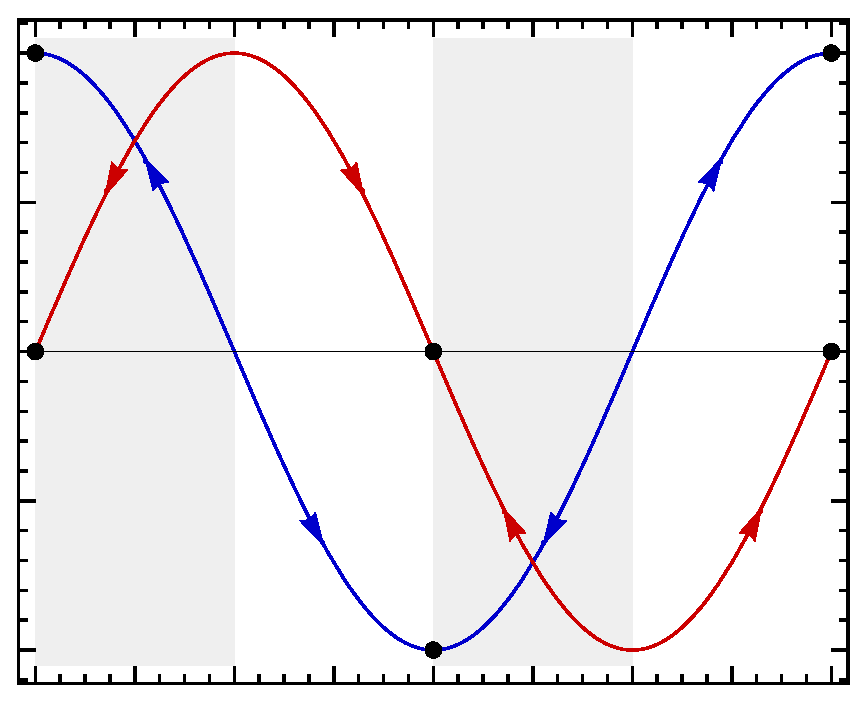
\includegraphics[width=0.8000\unitlength] 
  {\fdir/srg_toy_flow.eps}} 

%%%%% x-axis %%%%%%%%%%%%%%%%%%%%%%%%%%%%%%%%%%%%%%%%%%%%%%%%%%%%
\put(0.1200,0.1650){\parbox{0.2000\unitlength}{\centering $0$}} 
\put(0.2150,0.1650){\parbox{0.2000\unitlength}{\centering $\tfrac{\pi}{2}$}} 
\put(0.3100,0.1650){\parbox{0.2000\unitlength}{\centering $\pi$}} 
\put(0.4050,0.1650){\parbox{0.2000\unitlength}{\centering $\tfrac{3\pi}{2}$}} 
\put(0.5000,0.1650){\parbox{0.2000\unitlength}{\centering $2\pi$}} 
\put(0.5950,0.1650){\parbox{0.2000\unitlength}{\centering $\tfrac{5\pi}{2}$}} 
\put(0.6900,0.1650){\parbox{0.2000\unitlength}{\centering $3\pi$}} 
\put(0.7850,0.1650){\parbox{0.2000\unitlength}{\centering $\tfrac{7\pi}{2}$}} 
\put(0.8800,0.1650){\parbox{0.2000\unitlength}{\centering $4\pi$}} 

\put(0.2000,0.1000){\parbox{0.8000\unitlength}
  {\centering $\theta(s)$}} 

%%%%% y-axis %%%%%%%%%%%%%%%%%%%%%%%%%%%%%%%%%%%%%%%%%%%%%%%%%%%%
\put(0.0000,0.2270){\parbox{0.1900\unitlength}{\raggedleft$-1$}} 
\put(0.0000,0.3700){\parbox{0.1900\unitlength}{\raggedleft$-0.5$}} 
\put(0.0000,0.5110){\parbox{0.1900\unitlength}{\raggedleft$0$}} 
\put(0.0000,0.6560){\parbox{0.1900\unitlength}{\raggedleft$0.5$}} 
\put(0.0000,0.7990){\parbox{0.1900\unitlength}{\raggedleft$1$}} 

\put(0.0700,0.2000){{\color{white}.}}
\put(0.0700,0.2000){\begin{sideways}\parbox{0.6400\unitlength}
  {\centering $E_{-}(s),\; V(s)\,[\Omega]$}\end{sideways}} 

%%%%% plot label %%%%%%%%%%%%%%%%%%%%%%%%%%%%%%%%%%%%%%%%%%%%%%%%
\put(0.2500,0.7400){\parbox{0.7000\unitlength}
  {\raggedleft  }} 

%%%%% user stuff %%%%%%%%%%%%%%%%%%%%%%%%%%%%%%%%%%%%%%%%%%%%%%%%

%%%%%%%%%%%%%%%%%%%%%%%%%%%%%%%%%%%%%%%%%%%%%%%%%%%%%%%%%%%%%%%%%
\end{picture} 

    \begin{picture}(1.3000,0.8500)
      \put(0.0000,0.0000){%!TEX root = ../lnp.tex
\begin{picture}(1.0000,0.8400) 

%%%%% eps file %%%%%%%%%%%%%%%%%%%%%%%%%%%%%%%%%%%%%%%%%%%%%%%%%%
\put(0.2000,0.2000){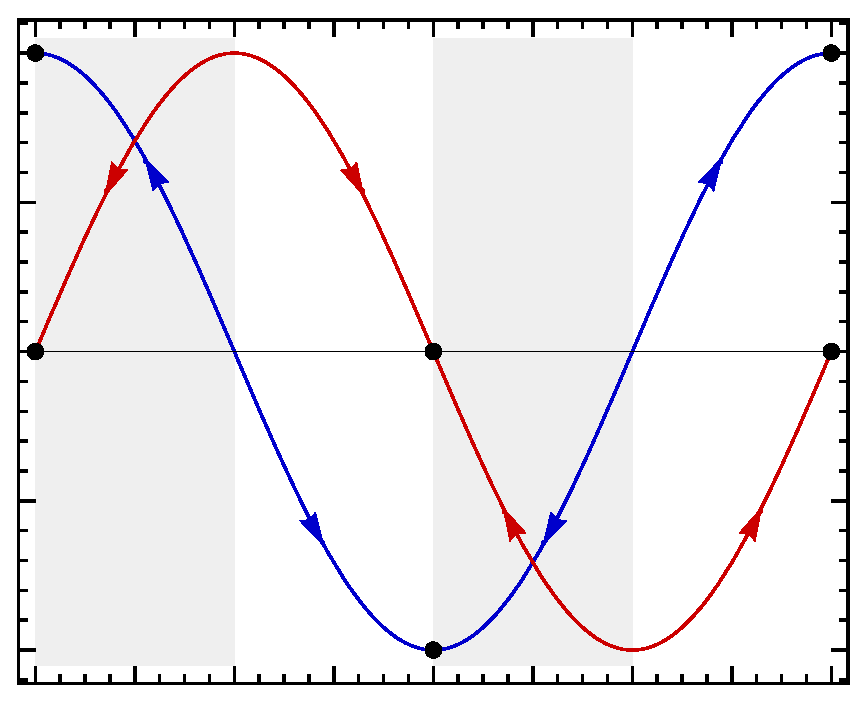
\includegraphics[width=0.8000\unitlength] 
  {\fdir/srg_toy_flow.eps}} 

%%%%% x-axis %%%%%%%%%%%%%%%%%%%%%%%%%%%%%%%%%%%%%%%%%%%%%%%%%%%%
\put(0.1200,0.1650){\parbox{0.2000\unitlength}{\centering $0$}} 
\put(0.2150,0.1650){\parbox{0.2000\unitlength}{\centering $\tfrac{\pi}{2}$}} 
\put(0.3100,0.1650){\parbox{0.2000\unitlength}{\centering $\pi$}} 
\put(0.4050,0.1650){\parbox{0.2000\unitlength}{\centering $\tfrac{3\pi}{2}$}} 
\put(0.5000,0.1650){\parbox{0.2000\unitlength}{\centering $2\pi$}} 
\put(0.5950,0.1650){\parbox{0.2000\unitlength}{\centering $\tfrac{5\pi}{2}$}} 
\put(0.6900,0.1650){\parbox{0.2000\unitlength}{\centering $3\pi$}} 
\put(0.7850,0.1650){\parbox{0.2000\unitlength}{\centering $\tfrac{7\pi}{2}$}} 
\put(0.8800,0.1650){\parbox{0.2000\unitlength}{\centering $4\pi$}} 

\put(0.2000,0.1000){\parbox{0.8000\unitlength}
  {\centering $\theta(s)$}} 

%%%%% y-axis %%%%%%%%%%%%%%%%%%%%%%%%%%%%%%%%%%%%%%%%%%%%%%%%%%%%
\put(0.0000,0.2270){\parbox{0.1900\unitlength}{\raggedleft$-1$}} 
\put(0.0000,0.3700){\parbox{0.1900\unitlength}{\raggedleft$-0.5$}} 
\put(0.0000,0.5110){\parbox{0.1900\unitlength}{\raggedleft$0$}} 
\put(0.0000,0.6560){\parbox{0.1900\unitlength}{\raggedleft$0.5$}} 
\put(0.0000,0.7990){\parbox{0.1900\unitlength}{\raggedleft$1$}} 

\put(0.0700,0.2000){{\color{white}.}}
\put(0.0700,0.2000){\begin{sideways}\parbox{0.6400\unitlength}
  {\centering $E_{-}(s),\; V(s)\,[\Omega]$}\end{sideways}} 

%%%%% plot label %%%%%%%%%%%%%%%%%%%%%%%%%%%%%%%%%%%%%%%%%%%%%%%%
\put(0.2500,0.7400){\parbox{0.7000\unitlength}
  {\raggedleft  }} 

%%%%% user stuff %%%%%%%%%%%%%%%%%%%%%%%%%%%%%%%%%%%%%%%%%%%%%%%%

%%%%%%%%%%%%%%%%%%%%%%%%%%%%%%%%%%%%%%%%%%%%%%%%%%%%%%%%%%%%%%%%%
\end{picture} 
}
      \put(1.0500,0.5000){\fbox{\parbox{0.2\unitlength}{\raggedright $E_{-}(s)$ \\[5pt] $V(s)$}}}
      \put(1.1800,0.5400){\thicklines\color{blue}\line(1,0){0.06}}
      \put(1.1800,0.4800){\thicklines\color{red}\line(1,0){0.06}}
    \end{picture}
  \end{center}
  \vspace{-20pt}
  \caption{\label{fig:srg_toy}
    $E_{-}(s)$ and $V(s)$ as a function of the flowing angle $\theta(s)$, in units of the
    flow invariant $\Omega$. Black dots and
    arrows the fixed points at $s\to\infty$ and the directions of the SRG flow, respectively,
    in the domains corresponding to specific sign combinations for $E_{-}(s)$ and $V(s)$ (see
    text).
  }
\end{figure}

%%%%%%%%%%%%%%%%%%%%%%%%%%%%%%%%%%%%%%%%%%%%%%%%%%%%%%%%%%%%%%%%%%%%%%
% SUBSECTION %%%%%%%%%%%%%%%%%%%%%%%%%%%%%%%%%%%%%%%%%%%%%%%%%%%%%%%%%
%%%%%%%%%%%%%%%%%%%%%%%%%%%%%%%%%%%%%%%%%%%%%%%%%%%%%%%%%%%%%%%%%%%%%%
\subsection{\label{sec:srg_pairing}The Pairing Model}

%
% SUBSUBSECTION %%%%%%%%%%%%%%%%%%%%%%%%%%%%%%%%%%%%%%%%%%%%%%%%%%%%%%
%
\subsubsection{Preliminaries}
\begin{table}[t]
  \begin{center}
      \begin{tabular*}{0.25\textwidth}{@{\extracolsep\fill}|c|c|r|r|}
      \hline 
      state & $p$ & $2s_z$ & $\varepsilon$
      \\ \hline 
      $0$ & $1$ & $ 1$ & $     0 $ \\ 
      $1$ & $1$ & $-1$ & $     0 $ \\ 
      $2$ & $2$ & $ 1$ & $ \delta$ \\ 
      $3$ & $2$ & $-1$ & $ \delta$ \\ 
      $4$ & $3$ & $ 1$ & $2\delta$ \\ 
      $5$ & $3$ & $-1$ & $2\delta$ \\ 
      $6$ & $4$ & $ 1$ & $3\delta$ \\ 
      $7$ & $4$ & $-1$ & $3\delta$ \\ \hline
      \end{tabular*}
  \end{center}
  \caption{\label{tab:srg_pairing_sp}Single-particle states and their quantum numbers and their energies from Eq.~(\ref{eq:def_pairing_hamiltonian}). The degeneracy for every quantum number $p$ is equal to 2 due to the two possible spin values.} 
\end{table}

As our second example for diagonalizing matrices by means of SRG flows, we will
consider the pairing model that was discussed in the context of Hartree-Fock and
beyond-HF methods in chapter \ref{chapter:cc}. In second quantization, the 
pairing Hamiltonian is given by
\begin{equation}\label{eq:def_pairing_hamiltonian}
  \HO = \delta \sum_{p \sigma} (p-1) a^{\dagger}_{p \sigma} a_{p\sigma}
        -\frac{1}{2}g \sum_{pq} a^{\dagger}_{p+}a^{\dagger}_{p-}a_{q-}a_{q+}\,,
\end{equation}
where $\delta$ controls the spacing of single-particle levels that are indexed
by a principal quantum number $p$ and their spin projection $\sigma$ (see 
Tab.~\ref{tab:srg_pairing_sp}), and $g$ the strength of the pairing interaction. 

We will consider the case of 4 particles in 8 single-particle states. Following
the Full Configuration Interaction (FCI) approach discussed in chapter \ref{chapter:cc},
we can construct a many-body basis of Slater determinants by placing
our 4 particles into the 8 single-particle basis states. Since each
single-particle state can only be occupied by one particle, there are
\begin{equation}
  \begin{pmatrix} 8 \\ 4\end{pmatrix} = 70
\end{equation}
unique configurations. The specific form of the pairing interaction
implies that the total spin projection $S_z = \sum_{n=1}^4 s_z^{(n)}$ 
is conserved, and the Hamiltonian will have a block diagonal structure.
The possible values for $S_z$ are $-2,-1,0,1,2$, depending on the number
of particles in states with spin up or spin down. The dimension can be
calculated via
\begin{equation}
 d_{S_z} = \begin{pmatrix} 4 \\ N_{+}\end{pmatrix} \times 
           \begin{pmatrix} 4 \\ N_{-}\end{pmatrix}\,,
\end{equation}
which yields 
\begin{equation}
 d_{\pm 2} = 1\,, \quad d_{\pm 1} = 16\,, \quad d_{0} = 36\,.
\end{equation}
Since the pairing interaction only couples pairs of single-particle 
states with the same principal quantum number but opposite spin
projection, it does not break pairs of particles that occupy such 
states --- in other words, the number of particle pairs is another
conserved quantity, which allows us to decompose the $S_z$ blocks
into even smaller sub blocks. As in chapter 8, we consider the $S_z=0$
sub block with two particle pairs, which is six-dimensional. In this
block, the Hamiltonian is represented by the matrix (suppressing
block indices)
\begin{equation}\label{eq:def_h_matrix}
  H = \begin{pmatrix}
  2\delta -g  &      -g/2  &       -g/2 &      -g/2 &      -g/2 &        0 \\ 
         -g/2 & 4\delta -g &       -g/2 &      -g/2 &        -0 &     -g/2 \\ 
         -g/2 &       -g/2 & 6\delta -g &         0 &      -g/2 &     -g/2 \\ 
         -g/2 &       -g/2 &          0 & 6\delta-g &      -g/2 &     -g/2 \\ 
         -g/2 &          0 &       -g/2 &      -g/2 & 8\delta-g &     -g/2 \\ 
            0 &       -g/2 &       -g/2 &      -g/2 &      -g/2 & 10\delta -g
  \end{pmatrix}\,.
\end{equation}

%
% SUBSUBSECTION %%%%%%%%%%%%%%%%%%%%%%%%%%%%%%%%%%%%%%%%%%%%%%%%%%%%%%
%
\subsubsection{SRG Flow for the Pairing Hamiltonian}
As in earlier sections, we split the Hamiltonian matrix \eqref{eq:def_h_matrix}
into diagonal and off-diagonal parts:
\begin{equation}
  H_d(s) = \mathrm{diag}(E_0(s)\,,\ldots,E_5(s))\,,\quad H_{od}(s) = H(s) - H_{d}(s)\,,
\end{equation}
with initial values defined by Eq.~\eqref{eq:def_h_matrix}. Since $H_d(s)$
is diagonal throughout the flow per construction, the Slater determinants
that span our specific subspace are the eigenstates of this matrix. In our 
basis representation, Eq.~\eqref{eq:opflow} can be written as
\begin{align}
  \totd{}{s}\matrixe{i}{\HO}{j}
  &=\sum_k\left(\matrixe{i}{\etaO}{k}\matrixe{k}{\HO}{j}-\matrixe{i}{\HO}{k}\matrixe{k}{\etaO}{j}\right)\notag\\
  &=-\left(E_i-E_j\right)\matrixe{i}{\etaO}{j}
    +\sum_k\left(\matrixe{i}{\etaO}{k}\matrixe{k}{\HO_{od}}{j}-\matrixe{i}{\HO_{od}}{k}\matrixe{k}{\etaO}{j}\right),
\end{align}
where $\matrixe{i}{\HO_{od}}{i}=0$ and block indices as well as the $s$-dependence
have been suppressed for brevity. The Wegner generator, Eq.~\eqref{eq:def_Wegner_general}, 
is given by
\begin{equation}
  \matrixe{i}{\etaO}{j}=\matrixe{i}{\comm{\HO_d}{\HO_{od}}}{j}=(E_i-E_j)\matrixe{i}{\HO_{od}}{j}\,,
\end{equation}
and inserting this into the flow equation, we obtain
\begin{align}
  \totd{}{s}\matrixe{i}{\HO}{j}
  =-\left(E_i-E_j\right)^2\matrixe{i}{\HO_{od}}{j}
  +\sum_k\left(E_i+E_j-2E_k\right)\matrixe{i}{\HO_{od}}{k}\matrixe{k}{\HO_{od}}{j}\,.\label{eq:schema_wegner}
\end{align}
Let us assume that the transformation generated by $\etaO$ truly suppresses 
$\HO_{od}$, and consider the asymptotic behavior for large flow parameters 
$s>s_0\gg0$. If $||\HO_{od}(s_0)||\ll 1$ in some suitable norm, the second 
term in the flow equation can be neglected compared to the first one. For
the diagonal and off-diagonal matrix elements, this implies
\begin{align}
  \totd{E_i}{s} &= \totd{}{s} \matrixe{i}{\HO_d}{i} = 2\sum_k (E_i - E_k) \matrixe{i}{\HO_{od}}{k}\matrixe{k}{\HO_{od}}{i}
  \approx0
\end{align}
and
\begin{align}
  \totd{}{s}\matrixe{i}{\HO}{j}
  \approx-\left(E_i-E_j\right)^2\matrixe{i}{\HO_{od}}{j}\,,
\end{align}
respectively. Thus, the diagonal matrix elements will be (approximately)
constant in the asymptotic region,
\begin{equation}
  E_i(s) \approx E_i(s_0)\,,\quad s>s_0\,,
\end{equation}
which in turn allows us to integrate the flow equation for the off-diagonal
matrix elements. We obtain
\begin{equation}\label{eq:def_hod_general}
  \matrixe{i}{\HO_{od}(s)}{j} \approx \matrixe{i}{\HO_{od}(s_0)}{j}\,e^{-(E_i-E_j)^2 (s-s_0)}\,, \quad s>s_0\,,
\end{equation}
i.e., the off-diagonal matrix elements are suppressed exponentially, as for the
$2\times2$ matrix toy problem discussed in the previous section. If the pairing
strength $g$ is sufficiently small that $\HO^2_{od}(0)\sim \mathcal{O}(g^2)$ can 
be neglected, we expect to see the exponential suppression of the off-diagonal 
matrix elements from the very onset of the flow. 

Our solution for the off-diagonal matrix elements, Eq.~\eqref{eq:def_hod_general},
shows that the characteristic decay scale for each matrix element is determined 
by the square of the energy difference between the states it couples, 
$(\Delta E_{ij})^2 = (E_i-E_j)^2$. Thus, states with larger energy differences
are decoupled before states with small energy differences, which means that 
the Wegner generator generates a proper renormalization group transformation.
Since we want to diagonalize \eqref{eq:def_h_matrix} in the present example,
we are only interested in the limit $s\to\infty$, and it does not really matter
whether the transformation is an RG or not. Indeed, there are alternative choices
for the generator which are more efficient in achieving the desired diagonalization
(see section \ref{sec:generator} and Refs.~\cite{Hergert:2016jk,Hergert:2016ng}).
The RG property will matter in our discussion of SRG-evolved nuclear interactions 
in the next section.

%
% SUBSUBSECTION %%%%%%%%%%%%%%%%%%%%%%%%%%%%%%%%%%%%%%%%%%%%%%%%%%%%%%
%
\subsubsection{Implementation}
We are now ready to discuss the implementation of the SRG flow for the pairing
Hamiltonian. The main numerical task is the integration of the flow equations,
a system of first order ODEs. Readers who are interested in learning the 
nuts-and-bolts details of implementing an ODE solver are referred to the excellent 
discussion in \cite{Press:2007vn}, while higher-level discussions of the algorithms
can be found, e.g., in \cite{Shampine:1975qq,Landau:2012zr,Hjorth-Jensen:2015mz}.
A number of powerful ODE solvers have been developed over the past decades and 
integrated into readily available libraries, and we choose to rely one of these 
here, namely ODEPACK (see \url{www.netlib.org/odepack} and 
\cite{Hindmarsh:1983pd,Radhakrishnan:1993fk,Brown:1989qd}). The SciPy package
provides convenient Python wrappers for the ODEPACK solvers.

The following source code shows the essential part of our Python implementation of
the SRG flow for the pairing model. The full program with additional features can 
be downloaded from 
\url{https://github.com/ManyBodyPhysics/LectureNotesPhysics/blob/master/doc/src/\pdir/python/srg_pairing/srg_pairing.py}.


\begin{lstlisting}
import numpy as np
from numpy import array, dot, diag, reshape
from scipy.linalg import eigvalsh
from scipy.integrate import odeint

# Hamiltonian for the pairing model
def Hamiltonian(delta,g):

  H = array(
      [[2*delta-g,    -0.5*g,     -0.5*g,     -0.5*g,    -0.5*g,          0.],
       [   -0.5*g, 4*delta-g,     -0.5*g,     -0.5*g,        0.,     -0.5*g ], 
       [   -0.5*g,    -0.5*g,  6*delta-g,         0.,    -0.5*g,     -0.5*g ], 
       [   -0.5*g,    -0.5*g,         0.,  6*delta-g,    -0.5*g,     -0.5*g ], 
       [   -0.5*g,        0.,     -0.5*g,     -0.5*g, 8*delta-g,     -0.5*g ], 
       [       0.,    -0.5*g,     -0.5*g,     -0.5*g,    -0.5*g, 10*delta-g ]]
    )

  return H

# commutator of matrices
def commutator(a,b):
  return dot(a,b) - dot(b,a)

# derivative / right-hand side of the flow equation
def derivative(y, t, dim):

  # reshape the solution vector into a dim x dim matrix
  H = reshape(y, (dim, dim))

  # extract diagonal Hamiltonian...
  Hd  = diag(diag(H))

  # ... and construct off-diagonal the Hamiltonian
  Hod = H-Hd

  # calculate the generator
  eta = commutator(Hd, Hod)

  # dH is the derivative in matrix form 
  dH  = commutator(eta, H)

  # convert dH into a linear array for the ODE solver
  dydt = reshape(dH, -1)
    
  return dydt


#------------------------------------------------------------------------------
# Main program
#------------------------------------------------------------------------------
def main():
  g     = 0.5
  delta = 1

  H0    = Hamiltonian(delta, g)
  dim   = H0.shape[0]

  # calculate exact eigenvalues
  eigenvalues = eigvalsh(H0)

  # turn initial Hamiltonian into a linear array
  y0  = reshape(H0, -1)                 

  # flow parameters for snapshot images
  flowparams = array([0.,0.001,0.01,0.05,0.1, 1., 5., 10.])

  # integrate flow equations - odeint returns an array of solutions,
  # which are 1d arrays themselves
  ys  = odeint(derivative, y0, flowparams, args=(dim,))

  # reshape individual solution vectors into dim x dim Hamiltonian
  # matrices
  Hs  = reshape(ys, (-1, dim,dim))
\end{lstlisting}


The routine \texttt{Hamiltonian} sets up the Hamiltonian matrix \eqref{eq:def_h_matrix}
for general values of $\delta$ and $g$. The right-hand side of the flow equation
is implemented in the routine \texttt{derivative}, which splits $H(s)$
in diagonal and off-diagonal parts, and calculates both the generator and
the commutator $\comm{\etaO}{\HO}$ using matrix products. Since the
interface of essentially all ODE libraries require the ODE system and
derivative to be passed as a one-dimensional array, NumPy's \texttt{reshape}
functionality used to rearrange these arrays into $6\times 6$ matrices 
and back again.

The main routine calls the ODEPACK wrapper \texttt{odeint}, passing 
the initial Hamiltonian as a one-dimensional array \texttt{y0} as well
as a list of flow parameters $s$ for which a solution is requested. The 
routine \texttt{odeint} returns these solutions as a list of arrays.

%
% SUBSUBSECTION %%%%%%%%%%%%%%%%%%%%%%%%%%%%%%%%%%%%%%%%%%%%%%%%%%%%%%
%
\subsubsection{A Numerical Example}
\begin{figure*}[t]
  \begin{center}
    \includegraphics[width=0.95\textwidth]{\fdir/{srg_pairing_delta1.0_g0.5}.pdf}
  \end{center}    
  \caption{\label{fig:srg_pairing}SRG evolution of the pairing Hamiltonian with
  $\delta=1, g=0.5$. The 
  figures show snapshots of the Hamiltonian's matrix representation at various 
  stages of the flow, indicated by the flow parameters $s$. Note the essentially 
  logarithmic scales of the positive and negative matrix elements, which are bridged
  by a linear scale in the vicinity of 0.}
\end{figure*}

As a numerical example, we solve the pairing Hamiltonian for $\delta=1.0$
and $g=0.5$. In Fig.~\ref{fig:srg_pairing}, we show snapshots of the matrix
$H(s)$ at different stages of the flow. We can nicely see how the SRG evolution
drives the off-diagonal matrix elements to zero. The effect becomes noticeable 
on our logarithmic color scale around $s=0.05$, where the outermost off-diagonal 
matrix elements start to lighten. At $s=0.1$, $H_{05}(s)$ has been reduced by
four to five orders of magnitude, and at $s=1.0$, essentially all of the 
off-diagonal matrix elements have been affected to some extent. Note that the
strength of the suppression depends on the distance from the diagonal, aside from 
$H_{05}$ itself, which has a slightly larger absolute value than $H_{04}$ and
$H_{15}$. The overall behavior is as expected from our approximate solution 
\eqref{eq:def_hod_general}, and the specific deviations can be explained by 
the approximate nature of that result. Once we have reached $s=10$, the matrix
is essentially diagonal, with off-diagonal matrix elements reduced to  
$10^{-10}$ or less. Only the $2\times2$ block spanned by the states labeled 2
and 3 has slightly larger off-diagonal matrix elements remaining, which is 
due to the degeneracy of the corresponding eigenvalues.

\begin{figure*}[t]
  \setlength{\unitlength}{\textwidth}
  \begin{picture}(1.0000,0.4000)
    \put(0.0300,0.0300){\includegraphics[width=0.45\unitlength]{\fdir/{srg_pairing_diag_delta1.0_g0.5}.pdf}}
    \put(0.0100,0.0400){\begin{sideways}\parbox{0.3500\unitlength}{\centering$ E_i, H_{ii}(s)$ }\end{sideways}}
    \put(0.0200,0.0150){\parbox{0.500\unitlength}{\centering$s$}}
    \put(0.5200,0.0300){\includegraphics[width=0.46\unitlength]{\fdir/{srg_pairing_diag-eval_delta1.0_g0.5}.pdf}}    
    \put(0.5000,0.0400){\begin{sideways}\parbox{0.3500\unitlength}{\centering$ H_{ii}(s) - E_i$ }\end{sideways}}
    \put(0.5200,0.0150){\parbox{0.500\unitlength}{\centering$s$}}

  \end{picture}
  \caption{\label{fig:srg_pairing_diags}SRG evolution of the pairing Hamiltonian
  with $\delta=1, g=0.5$. The left panel shows the diagonal matrix elements $H_{ii}(s)$ as a function of
  the flow parameter $s$ (dashed lines)  and
  the corresponding eigenvalues (solid lines), the right panel the difference of
  the two numbers. The color coding is the same in both panels.}
\end{figure*}

In Fig.~\ref{fig:srg_pairing_diags}, we compare the flowing diagonal matrix
elements $H_{ii}(s)$ to the eigenvalues of the pairing Hamiltonian. As
we have just mentioned, the pairing Hamiltonian has a doubly degenerate 
eigenvalue $E_2=E_3=6\delta-g$, which is why we see only five curves
in these plots. For our choice of parameters, the diagonal matrix elements
are already in fairly good agreement with the eigenvalues to begin with. Focusing
on the right-hand panel of the figure in particular, we see that $H_{00}$ (blue) 
and $H_{11}$ (red) approach their eigenvalues from above, while 
$H_{44}$ (orange) and $H_{55}$ (light blue) approach from below as we evolve
to large $s$. It is interesting that the diagonal matrix elements 
are already practically identical to the eigenvalues once we have 
integrated up to $s=1.0$, despite the non-vanishing off-diagonal matrix elements 
that are visible in the $s=1.0$ snapshot shown in Fig.~\ref{fig:srg_pairing}.

%%%%%%%%%%%%%%%%%%%%%%%%%%%%%%%%%%%%%%%%%%%%%%%%%%%%%%%%%%%%%%%%%%%%%%
% SUBSECTION %%%%%%%%%%%%%%%%%%%%%%%%%%%%%%%%%%%%%%%%%%%%%%%%%%%%%%%%%
%%%%%%%%%%%%%%%%%%%%%%%%%%%%%%%%%%%%%%%%%%%%%%%%%%%%%%%%%%%%%%%%%%%%%%
\subsection{Evolution of Nuclear Interactions}

%
% SUBSUBSECTION %%%%%%%%%%%%%%%%%%%%%%%%%%%%%%%%%%%%%%%%%%%%%%%%%%%%%%
%
\subsubsection{\label{sec:srg_opflow}Matrix and Operator Flows}
In our discussion of the schematic pairing model in the previous section, we 
have used SRG flows to solve the eigenvalue problem arising from a four-body 
Schr\"odinger equation, so we may want to use the same method for the more 
realistic case of $A$ nucleons interacting by nuclear $NN$, $3N$, etc. 
interactions (see chapter \ref{chapter:cc}). However, we quickly realize the
main problem of such an approach: Working in a full configuration interaction (FCI) 
picture
and assuming even a modest single-particle basis size, e.g., 50 proton and neutron 
states each, a basis for the description of a nucleus like $\nuc{O}{16}$ would 
naively have
\begin{equation}
 d(\nuc{O}{16}) = \begin{pmatrix} 50 \\ 8\end{pmatrix} \times 
           \begin{pmatrix} 50 \\ 8\end{pmatrix}
                = 2.88\times10^{17}
\end{equation}
configurations, i.e., we would need about 3 exabyte (EB) to store all the coefficients
of just one eigenvector in memory, and $7\times10^{17}$ EB if we were to construct
the complete Hamiltonian matrix! State-of-the-art methods for large-scale 
diagonalization are able to reduce the memory requirements and computational
effort significantly by exploiting matrix sparseness, and using modern versions of
Lanczos-Arnoldi \cite{Lanczos:1950sp,Arnoldi:1951kk} or Davidson algorithms 
\cite{Davidson:1989pi}, but nuclei in the vicinity of the oxygen isotopic 
chain are among the heaviest accessible with today's computational
resources (see, e.g., \cite{Yang:2013ly,Barrett:2013oq} and references therein).
A key feature of Lanczos-Arnoldi and Davidson methods is that the
Hamiltonian matrix only appears in the calculation
of matrix-vector products. In this way, an explicit construction of the Hamiltonian
matrix in the CI basis is avoided, because the matrix-vector product can be
calculated from the input $NN$ and $3N$ interactions that only require $\OC(n^4)$ 
and $\OC(n^6)$ storage, respectively, where $n$ is the size of the single-particle
basis (see section \ref{sec:imsrg}). However, the SRG flow of the previous section 
clearly forces us to construct
and store the Hamiltonian matrix in its entirety --- at best, we could save some
storage by resizing the matrix once its off-diagonal elements have been 
sufficiently suppressed.

Instead of trying to evolve the many-body Hamiltonian matrix, we therefore focus
on the Hamiltonian operator itself instead. Let us consider a nuclear Hamiltonian 
with a two-nucleon interaction for simplicity:
\begin{equation}
  \Hint = \Tint + \VO^{[2]}\,.
\end{equation}
Since nuclei are self-bound objects, we have to consider the intrinsic form of the 
kinetic energy, 
\begin{equation}
  \Tint \equiv \TO - \Tcm\,.
\end{equation}
It is straightforward to show that $\Tint$ can be written either as a sum of
one- and two-body operators,
\begin{equation}\label{eq:def_Tint_1B2B}
  \Tint= \left(1-\frac{1}{\AO}\right)\sum_{i}\frac{\pOV_i^2}{2m} - \frac{1}{\AO}\sum_{i<j}\frac{\pOV_{i}\cdot\pOV_{j}}{m}
\end{equation}
or as a pure two-body operator
\begin{equation}\label{eq:def_Tint_2B}
  \Tint= \frac{2}{\AO}\sum_{i<j}\frac{\qOV_{ij}^2}{2\mu}\,,\quad \qOV_{ij}\equiv\pOV_{i}-\pOV_{j}\,.
\end{equation}
Here, $\AO$ should be treated as a particle-number \emph{operator} (see \cite{Hergert:2009wh}),
and $\mu=m/2$ is the reduced nucleon mass (neglecting the proton-neutron mass difference).
Using Eq.~\eqref{eq:def_Tint_2B} for the present discussion, we can write the intrinsic 
Hamiltonian as
\begin{equation}\label{eq:def_Hint_2B}
  \Hint = \frac{2}{\AO}\sum_{i<j}\frac{\qOV_{ij}^2}{2\mu} + \sum_{i<j}\vO^{[2]}_{ij}\,,
\end{equation}
and directly consider the evolution of this operator via the flow equation
\eqref{eq:opflow}. It is customary to absorb the flow-parameter dependence 
completely into the interaction part of the Hamiltonian, and leave the kinetic
energy invariant --- in our previous examples, this simply amounts to moving the
$s-$dependent part of $\HO_d(s)$ into $\HO_{od}(s)$. We end up with a flow equation 
for the two-body interaction:
\begin{align}\label{eq:opflow_NN}
  \totd{}{s}v^{[2]}_{ij} &= \comm{\eta}{\vO^{[2]}_{ij}}\,.
\end{align}
In cases where we can expand the two-body interaction in terms of a finite algebra of
``basis'' operators, Eq.~\eqref{eq:opflow_NN} becomes a system of ODEs for the expansion 
coefficients, the so-called running couplings of the Hamiltonian, as explained
in earlier chapters of this book. An example is the toy problem discussed in section 
\ref{sec:srg_toy}: We actually expanded our $2\times2$ in terms of the algebra 
$\{\idO,\sigmaO_{1},\sigmaO_{2},\sigmaO_{3}\}$,
and related the matrix elements to the coefficients in this expansion. While 
the representation of the basis operators of our algebra would force us to use
extremely large matrices when we deal with an $A-$body system, we may be able
to capture the SRG flow completely with a small set of ODEs for the couplings 
of the Hamiltonian!

If we cannot identify a set of basis operators for the two-body interaction, we 
can still resort to representing it as a matrix between two-body states. For a given
choice of single-particle basis with size $n$, $\vO^{[2]}$ is then represented
by $\OC(n^4)$ matrix elements, as mentioned above. In general, we will then have
to face the issue of induced many-body forces, as discussed in section 
\ref{sec:srg_induced}.

%
% SUBSUBSECTION %%%%%%%%%%%%%%%%%%%%%%%%%%%%%%%%%%%%%%%%%%%%%%%%%%%%%%
%
\subsubsection{\label{sec:srg_nn}SRG in the Two-Nucleon System}

\begin{figure*}[t]
  \setlength{\unitlength}{\textwidth}
  \begin{center}
  \begin{picture}(0.9000,0.5100)
    \put(0.0000,0.0400){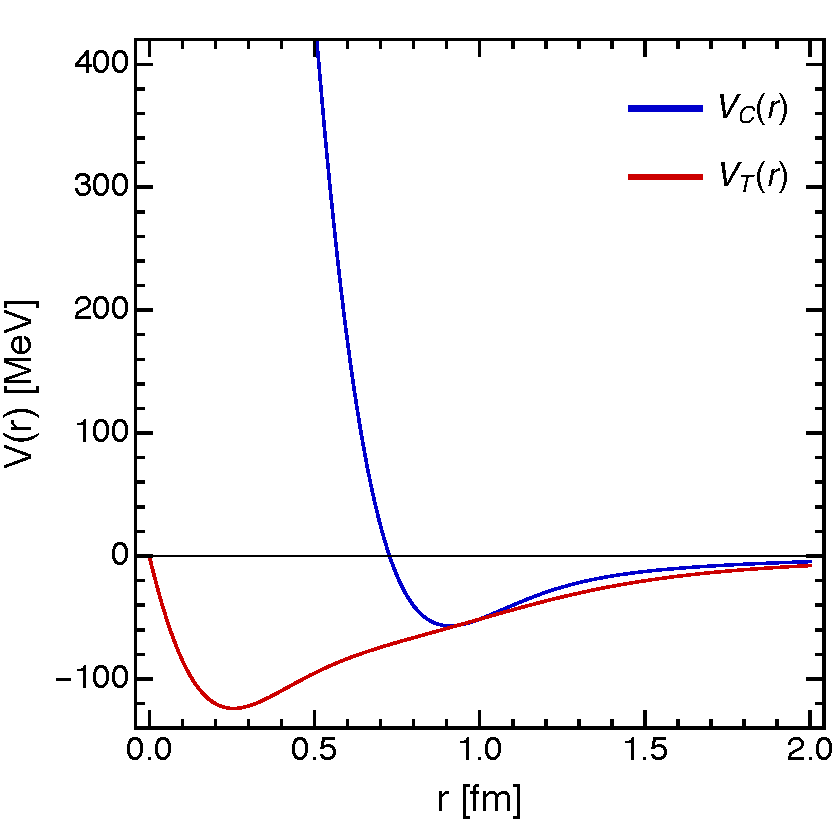
\includegraphics[width=0.45\unitlength]{\fdir/av18_st10_central_and_tensor.pdf}}
    \put(0.5000,0.2550){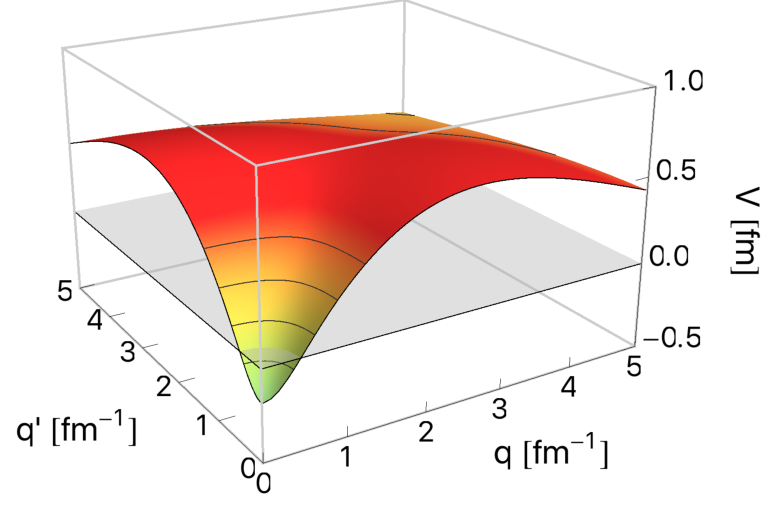
\includegraphics[width=0.40\unitlength]{\fdir/av18_srg0000_JLLST10010_meq.pdf}}
    \put(0.5000,0.0000){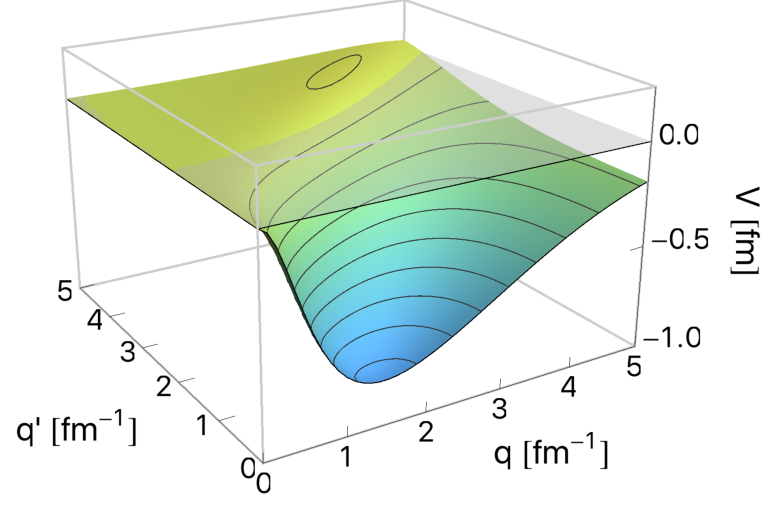
\includegraphics[width=0.40\unitlength]{\fdir/av18_srg0000_JLLST10210_meq.pdf}}
    \put(0.8700,0.4800){\fbox{\parbox{0.04\unitlength}{\raggedleft\large${}^3S_1$}}}
    \put(0.7900,0.2400){\fcolorbox{black}{white}{\parbox{0.12\unitlength}{\raggedleft\large${}^3S_1-{}^3D_1$}}}
  \end{picture}
  \end{center}
  \caption{\label{fig:av18}
    Repulsive core  and tensor force of the Argonne
    V18 $NN$ interaction \cite{Wiringa:1995or} in the $(S,T)=(1,0)$
    channel. In the left panel, the radial dependencies of the central ($V_C(r)$)  and tensor 
    components ($V_T(r)$) of Argonne V18 are shown, while the right panel shows its momentum 
    space matrix elements in the deuteron partial waves.
  }
\end{figure*}

Let us now consider the operator flow of the $NN$ interaction
in the two-nucleon system, Eq.~\eqref{eq:opflow_NN}. Since the nuclear Hamiltonian is invariant
under translations and rotations, it is most convenient to work in
momentum and angular momentum eigenstates of the form
\begin{equation}
  \ket{q(LS)JMTM_T}\,.
\end{equation}
Because of the rotational symmetry, the $NN$ interaction conserves
the total angular momentum quantum number $J$, and it is easy to show 
that the total spin $S$ of the nucleon pair is a conserved quantity as 
well. The
orbital angular momentum is indicated by the quantum number $L$,
and we remind our readers that $L$ is \emph{not} conserved, because
the nuclear tensor operator
\begin{equation}
  S_{ij}(\rOV,\rOV) = \frac{3}{\rOV^2}(\sigmaOV_i\cdot\rOV)(\sigmaOV_j\cdot\rOV)-\sigmaOV_i\cdot\sigmaOV_{j}
\end{equation}
can couple states with $\Delta L = \pm 2$. We
assume that the interaction is charge-dependent in the isospin channel
$T=1$, i.e., matrix elements will depend on the projection $M_T=-1,0,1$, 
which indicates the neutron-neutron, neutron-proton, and proton-proton 
components of the nuclear Hamiltonian. 


In figure \ref{fig:av18} we show features of the central 
and tensor forces of the Argonne V18 (AV18) interaction \cite{Wiringa:1995or}
in the $(S,T)=(1,0)$ channel, which has the quantum numbers of the deuteron. This 
interaction belongs to a group of so-called
realistic interactions that describe nucleon-nucleon scattering data
with high accuracy, but precede the modern chiral forces (see
chapter \ref{chapter:cc}, \cite{Epelbaum:2009ve,Machleidt:2011bh}). AV18
is designed to be maximally local in order to be a suitable input for
nuclear Quantum Monte Carlo calculations \cite{Carlson:2015lq,Gezerlis:2014zr,
Lynn:2016ec}. Because of the required locality, AV18 has a strong repulsive
core in the central part of the interaction. Like all $NN$ interactions,
it also has a strong tensor force that results from pion exchange. The
radial dependencies of these interaction components are shown in the left
panel of figure \ref{fig:av18}. 

When we switch to the momentum representation,
we see that the ${}^3S_1$ partial wave\footnote{We use the conventional partial wave
notation ${}^{2S+1}L_J$, where $L=0,1,2,\ldots$ is indicated by the letters 
$S,P,D,\ldots$. The isospin channel is fixed by requiring the antisymmetry
of the $NN$ wavefunction, leading to the condition $(-1)^{L+S+T}=-1$.} which
gives the dominant contribution to the deuteron wave function has strong
off-diagonal matrix elements, with tails extending over the entire shown
range and as high as $|\qOV| \sim 20\,\fmi$.
The matrix elements of the ${}^3S_1-{}^3D_1$ mixed partial wave, which
are generated exclusively by the tensor force, are sizable as well. The
strong coupling between states with low and high relative momenta forces
us to use large Hilbert spaces in few- and many-body calculations, even
if we are only interested in the lowest eigenstates. Methods like the 
Lanczos algorithm (see chapter \ref{chapter:cc} and \cite{Lanczos:1950sp})
extract eigenvalues and eigenvectors by repeatedly acting with the Hamiltonian
on an arbitrary starting vector in the many-body space, i.e., by repeated
matrix-vector products. Even if that vector only has low-momentum or low-energy 
components in the beginning, an interaction like AV18 will mix in high-momentum 
components even after a single matrix-vector multiplication, let alone tens 
or hundreds as in typical many-body calculations. Consequently, the 
eigenvalues and eigenstates of the nuclear Hamiltonian converge very slowly
with respect to the basis size of the Hilbert space, see, e.g., 
\cite{Barrett:2013oq}. To solve this problem, we perform an RG evolution of
the $NN$ interaction.

\begin{figure*}[t]
  \begin{center}
    \setlength{\unitlength}{\textwidth}
    \begin{picture}(0.9000,0.4100)
      \put(0.0000,0.0000){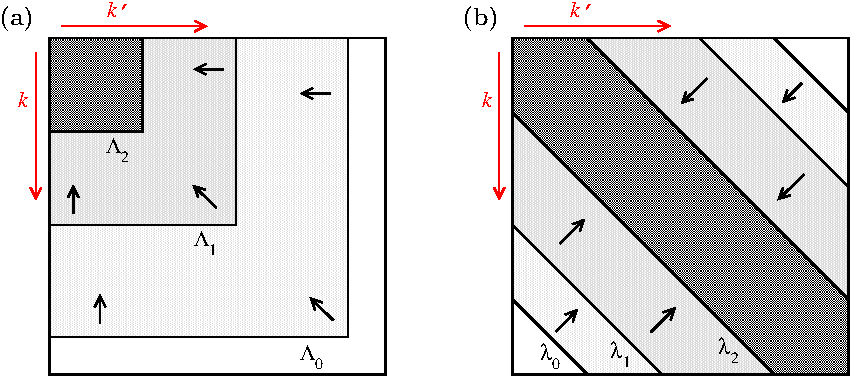
\includegraphics[width=0.9\textwidth]{\fdir/rg_evolution_schematic.pdf}}
      \put(0.0000,0.2850){\parbox{0.1\unitlength}{\colorbox{white}{\color{red}\large$q'$}}}
      \put(0.4900,0.2850){\parbox{0.1\unitlength}{\colorbox{white}{\color{red}\large$q'$}}}
      \put(0.1100,0.3860){\parbox{0.1\unitlength}{\colorbox{white}{\color{red}\large$q$}}}
      \put(0.6000,0.3860){\parbox{0.1\unitlength}{\colorbox{white}{\color{red}\large$q$}}}
    \end{picture}
  \end{center}
  \caption{\label{fig:schematic}Schematic illustration of two types of RG evolution 
    for $NN$ potentials in momentum space: (a) \Vlowk{} running in $\Lambda$, and 
    (b) SRG running in $\lambdaSRG$ (see main text). Here, $q$ and $q'$ denote the 
    relative momenta of the initial and final state, respectively. At each $\Lambda_i$ 
    or $\lambdaSRG_i$, the matrix elements outside of the corresponding 
    blocks or bands are negligible, implying that high- and low-momentum 
    states are decoupled.
  }
\end{figure*}

In figure \ref{fig:schematic}, we show examples for two types of RG evolution
that decouple the low- and momentum pieces of $NN$ interactions. The first
example, figure \ref{fig:schematic}(a), is a so-called  \emph{RG decimation}, 
in which the interaction is evolved to decreasing cutoff scales $\Lambda_0 > \Lambda_1 > \Lambda_2$, 
and high-momentum modes are ``integrated out''. This is the so-called \Vlowk{}
approach, which was first used in nuclear physics in the early 2000s 
\cite{Bogner:2003os,Bogner:2010pq}. Note that the resulting low-momentum 
interaction is entirely confined to states with relative momentum $q\leq\Lambda$.
In contrast, figure \ref{fig:schematic}(b) shows the SRG evolution of the $NN$ interaction
to a band-diagonal shape via the flow equation \eqref{eq:opflow_NN}, using a 
generator built from the relative kinetic energy in the two-nucleon system \cite{Bogner:2007od,Bogner:2010pq}:
\begin{equation}\label{eq:def_srg_generator}
  \eta(\lambda) \equiv \comm{\frac{\qOV^2}{2\mu}}{v(\lambda)}\,.
\end{equation}
Instead of the flow parameter $s$, we have parameterized the evolution by 
$\lambdaSRG=s^{-1/4}$, which has the dimensions of a momentum in natural units. 
Note that the generator \eqref{eq:def_srg_generator} would vanish if the
interaction were diagonal in momentum space. As suggested by figure 
\ref{fig:schematic}(b), $\lambdaSRG$ is a measure for the ``width'' of the 
band in momentum space. Thus, momentum transfers between nucleons are limited 
according to
\begin{equation}\label{eq:momentum_transfer}
  Q\equiv |\qOV' - \qOV| \lesssim \lambdaSRG\,,
\end{equation} 
and low- and high-lying momenta are decoupled as $\lambdaSRG$ is decreased. 

Equation \eqref{eq:momentum_transfer} implies that the spatial resolution scale
of an SRG-evolved interaction (or a \Vlowk{} if we determine the maximum
momentum transfer in the low-momentum block) is $\sim 1/Q \geq 1\lambdaSRG$,
i.e., only long-ranged components of the $NN$ interaction are resolved explicitly
and short-range components of the interaction can just as well be replaced 
by contact interactions \cite{Lepage:1997py,Bogner:2003os,Holt:2004ux,Bogner:2010pq}.
This is the reason why the realistic $NN$ interactions that accurately 
describe $NN$ scattering data collapse to a universal long-range interaction
when RG-evolved, namely one-pion exchange (OPE). This universal behavior emerges
in the range $1.5\,\fmi\leq\lambdaSRG\leq2.5\,\fmi$. Any further evolution to
lower $\lambdaSRG$ starts to remove pieces of OPE, and eventually generates a 
pion-less theory that is essentially parameterized in terms of contact 
interactions. While it is possible to implement such an evolution in
the two-body system without introducing pathological behavior \cite{Wendt:2011ys},
such an interaction must be complemented by strong induced many-nucleon
forces once it is applied in finite nuclei, as discussed in section \ref{sec:srg_induced}.
For this reason, $NN$ interactions are only ever evolved to the aforementioned
range of $\lambdaSRG$ values.

Nowadays, SRG evolutions are 
preferred over \Vlowk{} style decimations in nuclear many-body theory, because 
they can be readily extended to $3N,\ldots$ interactions and to general 
observables 
\cite{Bogner:2010pq,Anderson:2010br,Schuster:2014oq,More:2015bx,Jurgenson:2009bs,Hebeler:2012ly,Wendt:2013ys}. 
Moreover, we could easily achieve a block decoupling as in 
figure~\ref{fig:schematic}(a) by using a generator like \cite{Anderson:2008hx}
\begin{equation}\label{eq:def_srg_generator_PQ}
  \eta(\lambda) \equiv \comm{\underbrace{P_{\Lambda}H(\lambda)P_{\Lambda}+Q_{\Lambda}H(\lambda)Q_{\Lambda}}_{\equiv H_d(\lambda)}}{H(\lambda)}\,.
\end{equation}
where the projection operators $P_\Lambda$ and $Q_\Lambda$ partition the
relative momentum basis in states with $|\qOV|\leq\Lambda$ and $|\qOV|>\Lambda$,
respectively. In this case, $\lambda$ is an auxiliary parameter that is eliminated
by evolving $\lambda\to0$, just like we evolved $s\to\infty$ in sections \ref{sec:srg_toy}
and \ref{sec:srg_pairing}. 

%
% SUBSUBSECTION %%%%%%%%%%%%%%%%%%%%%%%%%%%%%%%%%%%%%%%%%%%%%%%%%%%%%%
%
\subsubsection{\label{sec:srg_nn_flow}Implementation of the Flow Equations}
We are now ready to implement the flow equations for the $NN$ interaction in
the momentum-space partial-wave representation. Using basis states that 
satisfy the orthogonality and completeness relations
\begin{equation}
  \braket{qLSJMTM_T}{q'L'S'J'M'T'M'_T} = 
    \frac{\delta(q-q')}{qq'}\delta_{LL'}\delta_{SS'}\delta_{JJ'}\delta_{MM'}\delta_{TT'}\delta_{M_TM'_T}
\end{equation}
and
\begin{equation}
  \idO = \sum_{LSJMTM_T}\int_0^\infty dq\,q^2 \ket{qLSJMTM_T}\bra{qLSJMTM_T}\,,
\end{equation}
respectively, we obtain \cite{Bogner:2007od,Bogner:2010pq}
\begin{align}
  \left(-\frac{\lambda^5}{4}\right)\frac{d\matrixe{qL}{\vO}{q'L'}}{d\lambda} =&- (q^2 - q'^{2})^2
  \matrixe{qL}{\vO}{q'L'}
  \notag\\
    &+ \sum_{\bar{L}}\int_0^{\infty}dp p^2\,
      (q^2 + q'{}^2 - 2p^2)\matrixe{qL}{\vO}{p\bar{L}}
      \matrixe{p\bar{L}}{\vO}{q'L'}\,,\label{eq:flow_nn}
\end{align}
where we have used scattering units ($\hbar^2/m=1$) and suppressed
the $\lambda$-dependence of $\vO$ as well as the conserved quantum 
numbers for brevity. Note that a prefactor $-\lambda^5/4$ 
appears due or change of variables from $s$ to $\lambda$. 

We can turn this integro-differential equation back into a matrix 
flow equation by discretizing the relative momentum variable, e.g.,
on uniform or Gaussian quadrature meshes. The matrix elements of the 
relative kinetic energy operator are then simply given by
\begin{equation}
  \matrixe{q_iL}{\tO}{q_jL'}=q_i^2 \delta_{q_iq_j}\delta_{LL'}\,
\end{equation}
(with $\hbar^2/m=1$). The discretization turns the integration
into a simple summation,
\begin{equation}
  \int_0^\infty dq\,q^2\;\rightarrow\;\sum_{i}w_i q^2_i\,,
\end{equation}
where the weights $w_i$ depend on our choice of mesh. For a uniform
mesh, all weights are identical and correspond to the mesh spacing,
while for Gaussian quadrature rules the mesh points and weights have
to be determined numerically \cite{Press:2007vn}. For convenience,
we absorb the weights and $q^2$ factors from the integral measure into 
the interaction matrix element,
\begin{equation}
  \matrixe{q_iL}{\overline{v}}{q_jL'} \equiv \sqrt{w_iw_j}q_i q_j\matrixe{q_iL}{\vO}{q_jL'}\,.
\end{equation}
The discretized flow equation then be written as
\begin{equation}\label{eq:flow_nn_discrete}
  \totd{}{\lambda} \matrixe{q_iL}{\overline{v}}{q_jL'} = - \frac{4}{\lambda^5}
    \matrixe{q_i}{\comm{\comm{\tO}{\overline{v}}}{\tO+\overline{v}}}{q_jL'}\,.
\end{equation}

We can solve Eq.~\eqref{eq:flow_nn_discrete} using a modified version of our 
Python code for the pairing model, discussed in section \ref{sec:srg_pairing}.
The Python code and sample inputs can be downloaded from 
\url{https://github.com/ManyBodyPhysics/LectureNotesPhysics/blob/master/doc/src/\pdir/python/srg_nn}.
Let us briefly discuss the most important modifications.

First, we have a set of functions that read the momentum mesh
and the input matrix elements from a file:
\begin{lstlisting}
def uniform_weights(momenta):
  weights = np.ones_like(momenta)
  weights *= abs(momenta[1]-momenta[0])
  return weights

def read_mesh(filename):
  data = np.loadtxt(filename, comments="#")  
  dim  = data.shape[1]
  
  momenta = data[0,:dim]

  return momenta
  
def read_interaction(filename):
  data = np.loadtxt(filename, comments="#")  
  dim  = data.shape[1]
  V = data[1:,:dim]
  return V
\end{lstlisting}

The matrix element files have the following format:
\begin{lstlisting}
# momentum space matrix elements 
# partial wave J=1, L=0/0, S=1, T=0, MT=0 
# 
# momentum grid [fm^-1]
0.000000 0.050000 0.100000 0.150000 0.200000 0.250000 0.300000 0.350000 0.400000 0.450000 
0.500000 0.550000 0.600000 0.650000 0.700000 0.750000 0.800000 0.850000 0.900000 0.950000 
...
6.300000 6.350000 6.400000 6.450000 6.500000 6.550000 6.600000 6.650000 6.700000 6.750000 
6.800000 6.850000 6.900000 6.950000 7.000000 
#
# matrix elements [MeV fm^3] 
-36.94918 -36.83554 -36.49896 -35.95649 -35.23306 -34.35875 -33.36536 -32.28337 -31.13985 
-29.95722 -28.75281 -27.53904 -26.32400 -25.11217 -23.90513 -22.70231 -21.50158 -20.29973 
...
0.00000   0.00000   0.00000   0.00000   0.00000   0.00000   0.00000   0.00000   0.00000   
0.00000   0.00000   0.00000   0.00000   0.00000   0.00000   0.00000   0.00000   0.00000
\end{lstlisting}
Comments, indicated by the \texttt{\#} character, are ignored. The first set
of data is a row containing the mesh points. Here, we have $141$ points in total,
ranging from $0$ to $7\,\fmi$ with a spacing of $0.05\,\fmi$. The range of momenta
is sufficient for the chiral $NN$ interaction we use in our example, the \NNNLO{} 
potential by Entem and Machleidt with cutoff $\Lambda=500\,\MeV$ \cite{Entem:2003th,Machleidt:2011bh}, 
which is considerably softer than the AV18 interaction discussed above. This is followed
by a simple $141 \times 141$ list of the matrix elements. It is straightforward
to adapt the format and I/O routines to Gaussian quadrature meshes by including
mesh points (i.e., the abscissas) and weights in the data file.

The derivative routine is almost unchanged, save for the prefactor due to the
use of $\lambda$ instead of $s$ to parameterize the flow, and the treatment of
the kinetic energy operator as explicitly constant:
\begin{lstlisting}
def derivative(lam, y, T):
# def derivative(y, lam, T):
  dim = T.shape[0]

  # reshape the solution vector into a dim x dim matrix
  V = reshape(y, (dim, dim))

  # calculate the generator
  eta = commutator(T, V)

  # dV is the derivative in matrix form 
  dV  = -4.0/(lam**5) * commutator(eta, T+V)

  # convert dH into a linear array for the ODE solver
  dydt = reshape(dV, -1)
    
  return dydt
\end{lstlisting}

In the main routine of the program, we first set up the mesh and 
then proceed to read the interaction matrix elements for the 
different partial waves.
We are dealing with a coupled-channel problem because
the tensor forces connects partial waves with $\Delta L=2$
in all $S=1$ channels. In our example, we restrict ourselves
to the partial waves that contribute to the deuteron bound
state, namely ${}^3S_1$, ${}^3D_1$,
and ${}^3S_1-{}^3D_1$. Indicating the orbital angular momenta
of these partial waves by indices, we have
\begin{equation}
  \mathbf{T}=
  \begin{pmatrix} 
      \;t\; &   \\
        &  \;t\;
  \end{pmatrix}\,,
  \quad
  \mathbf{V}=
  \begin{pmatrix} 
      \;\overline{v}_{00}\;       &  \;\overline{v}_{02}\; \\
      \;\overline{v}^\dag_{02}\;  &  \;\overline{v}_{22}\;
  \end{pmatrix}\,,
\end{equation}
where 
\begin{equation}
  t = \mathrm{diag}\left(q_0^2,\ldots,q_\text{max}^2\right)\,,
\end{equation}
since the kinetic energy is independent of $L$. As soon as we pass 
from the $S-$ into the $D-$ wave in either the
rows or the columns, the momentum mesh simply starts from the
lowest mesh point again. We use \texttt{NumPy}'s, \texttt{hstack()} 
and \texttt{vstack()} functions to assemble the interaction matrix
from the partial-wave blocks:

\begin{lstlisting}
def main():
...
  
  # read individual partial waves
  partial_waves=[]
  for filename in ["n3lo500_3s1.meq", "n3lo500_3d1.meq", "n3lo500_3sd1.meq"]:
    partial_waves.append(read_interaction(filename))
    # print partial_waves[-1].shape

  # assemble coupled channel matrix
  V = np.vstack((np.hstack((partial_waves[0], partial_waves[2])), 
                 np.hstack((np.transpose(partial_waves[2]), partial_waves[1]))
                ))

  # switch to scattering units
  V = V/hbarm
...
\end{lstlisting}

As discussed earlier, we work in scattering units with $\hbar^2/m=1$. Thus,
we have to divide the input matrix elements by this factor. We also need to
absorb the weights and explicit momentum factors into the interaction matrix.
It is convenient to define a conversion matrix for this purpose, which can
be multiplied element-wise with the entries of $\mathbf{V}$ using the 
regular \texttt{*} operator (recall that the matrix product is implemented
by the \texttt{NumPy} function \texttt{dot}).

% \begin{lstlisting}
% ...
%   conversion_matrix = np.zeros_like(T)
%   for i in range(dim):
%     for j in range(dim):
%       # Regularize the conversion matrix at zero momentum - set elements
%       # to machine precision so we can invert the matrix for plots etc.
%       # Note that momentum values are positive, by construction.
%       qiqj = max(np.finfo(float).eps, momenta[i]*momenta[j])
%       conversion_matrix[i,j] = qiqj*sqrt(weights[i]*weights[j])
% ...
% \end{lstlisting}

Since we changed variables from $s$ to $\lambda$, we now start the
integration at $\lambda=\infty$, or $\lambda\gg 1\fmi$ in practice.
As discussed above, we do not evolve all the way to $\lambda=0\,\fmi$,
but typically stop before we start integrating out explicit pion
physics, e.g., at $\lambda=1.5\,\fmi$. For typical $NN$ interactions,
especially those with a hard core like AV18, the flow equations tend
to become stiff because they essentially depend on cubic products of
the kinetic energy and interaction. For this reason, we use \texttt{SciPy}'s
\texttt{ode()} class, which provides access to a variety of solvers
and greater control over the parameters of the integration process.
Specifically, we choose the VODE solver package and its 5th-order 
Backward Differentiation method \cite{Brown:1989wj}, which is 
efficient and works robustly for a large variety of input interactions.

\begin{lstlisting}
...
  lam_initial = 20.0
  lam_final = 1.5

  # integrate using scipy.ode instead of scipy.odeint - this gives
  # us more control over the solver
  solver = ode(derivative,jac=None)

  # equations may get stiff, so we use VODE and Backward Differentiation
  solver.set_integrator('vode', method='bdf', order=5, nsteps=1000)
  solver.set_f_params(T)
  solver.set_initial_value(y0, lam_initial)

...
\end{lstlisting}

Finally, we reach the loop that integrates the ODE system. We request
output from the solver in regular intervals, reducing these intervals
as we approach the region of greatest practical interest, 
$1.5\,\fmi\leq \lambda \leq 2.5\,\fmi$: 

\begin{lstlisting}
...
  while solver.successful() and solver.t > lam_final:
    # adjust the step size in different regions of the flow parameter
    if solver.t >= 6.0:
      ys = solver.integrate(solver.t-1.0)
    elif solver.t >= 2.5:
      ys = solver.integrate(solver.t-0.5)
    elif solver.t < 2.5 and solver.t >= lam_final:
      ys = solver.integrate(solver.t-0.1)

    # add evolved interactions to the list
    flowparams.append(solver.t)
    Vtmp = reshape(ys,(dim,dim))
    Vs.append(Vtmp)

    print "%8.5f %14.8f"%(solver.t, eigvalsh((T + Vtmp)*hbarm)[0])

...
\end{lstlisting}

Of course, the ODE solver will typically take several hundred adaptive 
steps to propagate the solution with the desired accuracy between successive 
requested values of $\lambda$. At the end of each external 
step, we diagonalize the evolved Hamiltonian
and check whether the lowest eigenvalue, i.e., the deuteron binding
energy, remains invariant within the numerical tolerances we use for
the ODE solver. To illustrate the evolution of the $NN$ interaction, 
the code will also generate a sequence of matrix plots at the
desired values of $\lambda$, similar to figure \ref{fig:srg_pairing}
for the pairing Hamiltonian.

%
% SUBSUBSECTION %%%%%%%%%%%%%%%%%%%%%%%%%%%%%%%%%%%%%%%%%%%%%%%%%%%%%%
%
\subsubsection{\label{sec:srg_n3lo}Example: Evolution of a Chiral $NN$ Interaction}


\begin{figure*}[t]
  \setlength{\unitlength}{\textwidth}
  \begin{picture}(1.0000,1.0500)
    \put(0.0000,0.0000){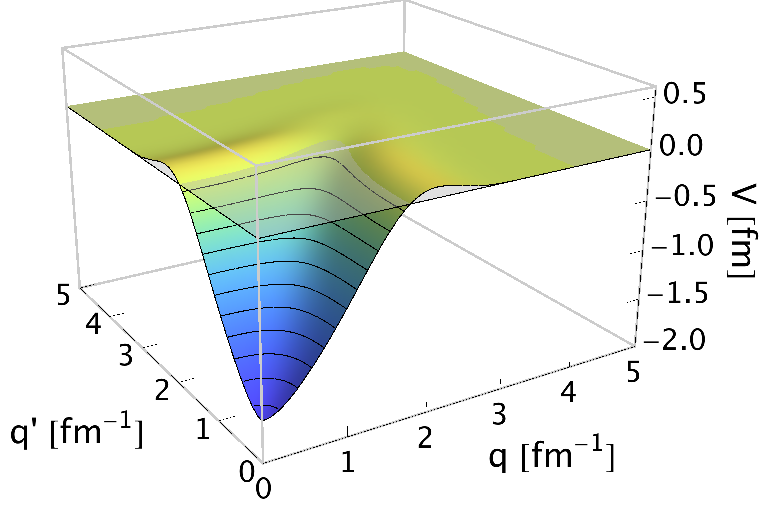
\includegraphics[width=0.5\unitlength]{\fdir/n3lo_srg0625_JLLST10010_meq.pdf}}
    \put(0.5500,0.0000){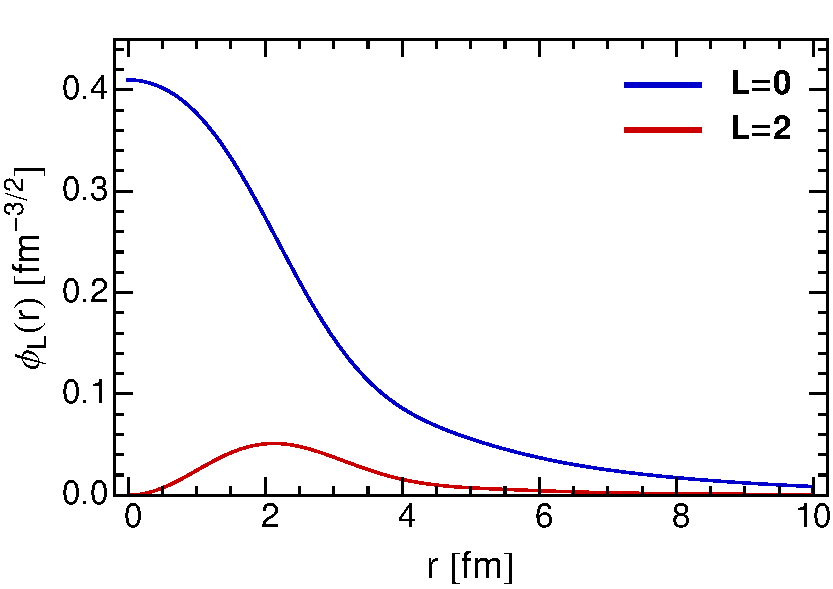
\includegraphics[width=0.45\unitlength]{\fdir/n3lo_srg0625_deuteron.pdf}}
    \put(0.0000,0.3500){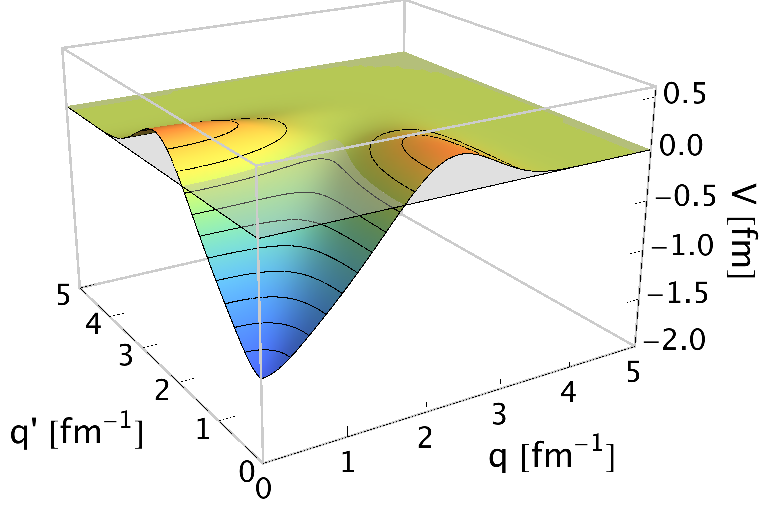
\includegraphics[width=0.5\unitlength]{\fdir/n3lo_srg0123_JLLST10010_meq.pdf}}
    \put(0.5500,0.3500){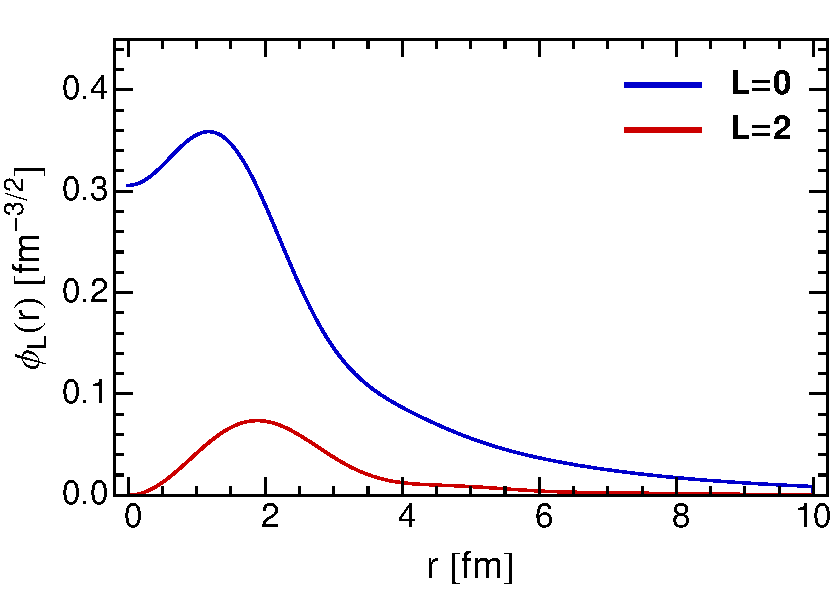
\includegraphics[width=0.45\unitlength]{\fdir/n3lo_srg0123_deuteron.pdf}}
    \put(0.0000,0.7000){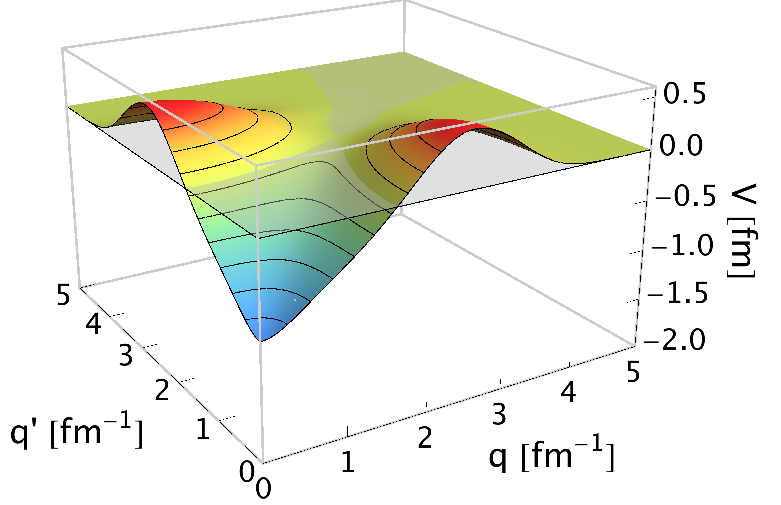
\includegraphics[width=0.5\unitlength]{\fdir/n3lo_srg0000_JLLST10010_meq.pdf}}
    \put(0.5500,0.7000){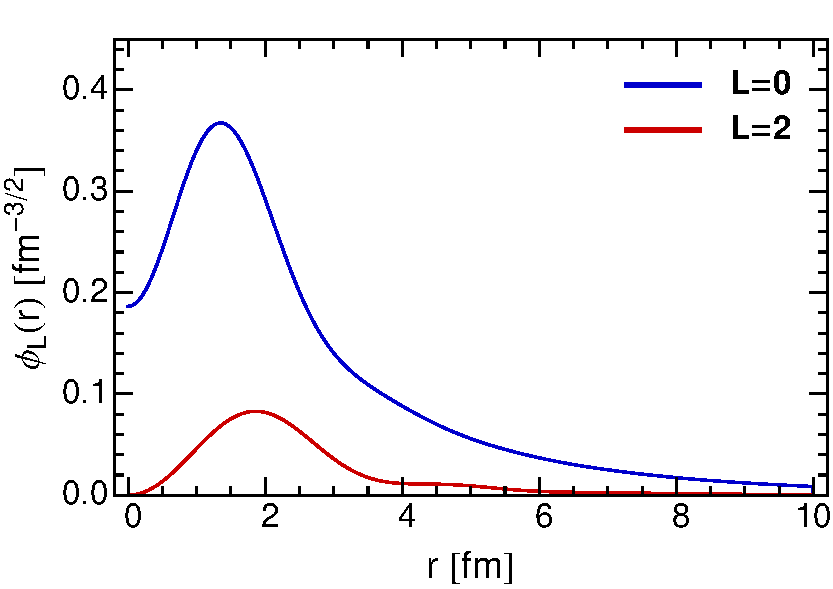
\includegraphics[width=0.45\unitlength]{\fdir/n3lo_srg0000_deuteron.pdf}}
    \put(0.0000,1.0000){\fcolorbox{black}{white}{\parbox{0.15\unitlength}{\centering\large``$\lambda = \infty$''}}}
    \put(0.0000,0.6500){\fcolorbox{black}{white}{\parbox{0.15\unitlength}{\centering\large$\lambda = 3\,\fmi$}}}
    \put(0.0000,0.3000){\fcolorbox{black}{white}{\parbox{0.15\unitlength}{\centering\large$\lambda = 2\,\fmi$}}}
  \end{picture}
  \\[10pt]
  \caption{\label{fig:vsrg_momentum}SRG evolution of the chiral \NNNLO{} nucleon-nucleon interaction
  by Entem and Machleidt, with initial cutoff $\Lambda=500\,\MeV$ \cite{Entem:2003th,Machleidt:2011bh}. 
  In the left column, we show the
  momentum-space matrix elements of the interaction in the ${}^3S_1$ partial wave for different values
  of the SRG resolution scale $\lambdaSRG$. The top-most row shows the initial interaction at $s=0\,\fm^4$\,,
  i.e., ``$\lambda=\infty$''. In the right column, we show the $S-$ and $D-$wave components
  of the deuteron wave function that is obtained by solving the Schr\"odinger equation with the corresponding
  SRG-evolved interaction.}
\end{figure*}

As an example of a realistic application, we discuss the SRG evolution of the
chiral \NNNLO{} nucleon-nucleon interaction by Entem and Machleidt with initial 
cutoff $\Lambda=500\,\MeV$ \cite{Entem:2003th,Machleidt:2011bh}. The momentum-space
matrix elements of this interaction in the deuteron partial waves are distributed
with the Python code discussed in the previous section.

In the top row of figure \ref{fig:vsrg_momentum}, we show the matrix elements
of the initial interaction in the ${}^3S_1$ partial wave; the ${}^3S_1-{}^3D_1$
and ${}^3D_1$ are not shown to avoid clutter. Comparing the matrix elements to
those of the AV18 interaction we discussed in section \ref{sec:srg_nn}, shown
in fig.~\ref{fig:av18}, we note that the chiral interaction has much weaker
off-diagonal matrix elements to begin with. While the AV18 matrix elements
extend as high as $|\qOV|\sim 20\,\fmi$, the chiral interaction has no appreciable
strength in states with $|\qOV|\sim 4.5\,\fmi$. In nuclear physics jargon, 
AV18 is a much harder interaction than the chiral interaction because of 
the former's strongly repulsive core. By evolving the initial interaction
to $3\,\fmi$ and then to $2\,\fmi$, the offdiagonal matrix elements are 
suppressed, and the interaction is almost entirely contained in a block
of states with $|\qOV|\sim 2\,\fmi$, except for a weak diagonal ridge.

Next to the matrix elements, we also show the deuteron wave functions
that we obtain by solving the Schr\"odinger equation with the initial
and SRG-evolved chiral interactions. For the unevolved $NN$ interaction,
the $S-$wave ($L=0$) component of the wave function is 
suppressed at small relative distances, which reflects short-range 
correlations between the nucleons. (For AV18, the $S-$wave component of 
the deuteron wave function vanishes at $r=0\,\fm$ due to the hard core.)
There is also a significant $D-$wave ($L=2$) admixture due to the tensor interaction.
As we lower the resolution scale, the ``correlation hole'' in the wave
function is filled in, and all but eliminated once we reach 
$\lambdaSRG=2.0\,\fmi$. The $D-$wave admixture is reduced significantly,
as well, because the evolution suppresses the 
matrix elements in the ${}^3S_1-{}^3D_1$ wave, which are responsible
for this mixing \cite{Bogner:2010pq}. Focusing just on the $S-$wave,
the wave function is extremely simple and matches what we would expect
for two almost independent, uncorrelated nucleons. The Pauli principle
does not affect the coordinate-space part of the wave function here 
because the overall antisymmetry of the deuteron wave function is ensured 
by its spin and isospin parts.

Let us dwell on the removal of short-range correlations from
the wave function for another moment, and consider the exact eigenstates of
the initial $NN$ Hamiltonian, 
\begin{equation}
  \HO(0) \ket{\psi_n} = E_n \ket{\psi_n}\,.
\end{equation}
The eigenvalues are invariant under a unitary transformation, e.g.,
an SRG evolution,
\begin{equation}
  \HO(\lambda)\UO(\lambda)\ket{\psi_n} \equiv \UO(\lambda) \HO(0) \UUO(\lambda) \UO(\lambda)\ket{\psi_n} 
    = E_n \UO(\lambda) \ket{\psi_n}\,.
\end{equation}
We can interpret this equation as a shift of correlations from the
wave function into the effective, \emph{RG-improved} Hamiltonian. When
we solve the Schr\"odinger equation numerically, we can usually only
obtain an approximation $\ket{\phi_n}$ of the exact eigenstate. In 
the ideal case, this is merely due to finite-precision arithmetic on
a computer, but more often, we also have systematic approximations,
e.g., mesh discretizations, finite basis sizes, many-body truncations 
(think of the cluster operator in Coupled Cluster, for instance, cf.~
chapter \ref{chapter:cc}), etc.
If we use the evolved Hamiltonian $\HO(\lambda)$, we only need 
to approximate the transformed eigenstate,
\begin{equation}\label{eq:approx_eigenstate}
  \ket{\phi_n}\approx\UO(\lambda)\ket{\psi_n}\,
\end{equation}
instead of $\ket{\psi_n}$, which is often a less demanding task.
This is certainly true for our deuteron example at $\lambda=2.0\,\fmi$,
where we no longer have to worry about short-range correlations.

%
% SUBSUBSECTION %%%%%%%%%%%%%%%%%%%%%%%%%%%%%%%%%%%%%%%%%%%%%%%%%%%%%%
%
\subsubsection{\label{sec:srg_induced}Induced Interactions}

As discussed earlier in this section, our motivation for using the SRG to
decouple the low- and high-lying momentum components of $NN$ interactions 
is to improve the convergence of many-body calculations. The decoupling 
prevents the Hamiltonian from scattering nucleon pairs from low to high 
momenta or energies, which in turn allows configuration-space based methods 
to achieve convergence in much smaller Hilbert spaces than for a ``bare'',
unevolved interaction. This makes it possible to extend the reach of these
methods to heavier nuclei \cite{Roth:2011kx,Barrett:2013oq,Jurgenson:2013fk,Roth:2014fk,Hergert:2013ij,Hergert:2013mi,Hergert:2014vn,Hergert:2016jk,Hagen:2010uq,Roth:2012qf,Binder:2013zr,Binder:2014fk,Soma:2011vn,Soma:2013ys,Soma:2014fu,Soma:2014eu}.

In practical applications, we pay a prize for the improved convergence.
To illustrate the issue, we consider the Hamiltonian in a second-quantized 
form, assuming only a two-nucleon interaction for simplicity (cf.~Eq.~\eqref{eq:def_Hint_2B}):
\begin{equation}\label{eq:H}
  \Hint = \frac{1}{4}\sum_{pqrs} \matrixe{pq}{\frac{\qOV^2}{2\mu}+\vO}{rs}\aaO_p\aaO_q\aO_s\aO_r\,.
\end{equation}
If we plug the kinetic energy and interaction into the commutators in 
equations \eqref{eq:def_srg_generator} and \eqref{eq:opflow}, we obtain
\begin{equation}\label{eq:comm2B_vac}
  \comm{\aaO_i\aaO_j\aO_l\aO_k}{\aaO_p\aaO_q\aO_s\aO_r}=
  \delta_{lp}\aaO_i\aaO_j\aaO_q\aO_s\aO_r\aO_k + \aaO\aaO\aaO\aO\aO\aO
  -\delta_{lp}\delta_{kq}\aaO_i\aaO_j\aO_s\aO_r + \aaO\aaO\aO\aO\,, 
\end{equation}
where the terms with suppressed indices schematically stand for additional 
two- and three-body operators. Even if we start from a pure $NN$
interaction, the SRG flow will induce operators of higher rank, i.e., 
$3N$, $4N$, and in general up to $A$-nucleon interactions. Of course, 
these induced interactions are only probed if we study an $A$-nucleon 
system. If we truncate the SRG flow equations at the two-body level, 
the properties of the two-nucleon system are preserved, in particular
the $NN$ scattering phase shifts and the deuteron binding energy. A 
truncation at the three-body level ensures the invariance of observables 
in $A=3$ nuclei, e.g.~$\nuc{H}{3}$ and $\nuc{He}{3}$ ground-state energies, 
and so on. 
% Any truncation in the SRG flow equation will lead to a violation 
% of unitarity that manifests as a (residual) dependence of many-body 
% results on the resolution scale $\lambdaSRG$. By varying this parameter, 
% the size of the missing contributions can be assessed (see, e.g., \cite{Bogner:2010pq,
% Jurgenson:2009bs,Hebeler:2012ly,Roth:2011kx,Hergert:2013mi,Hergert:2013ij,Binder:2014fk,
% Soma:2014eu,Griesshammer:2015dp}).


\begin{figure*}[t]
  \setlength{\unitlength}{\textwidth}
  \begin{center}
    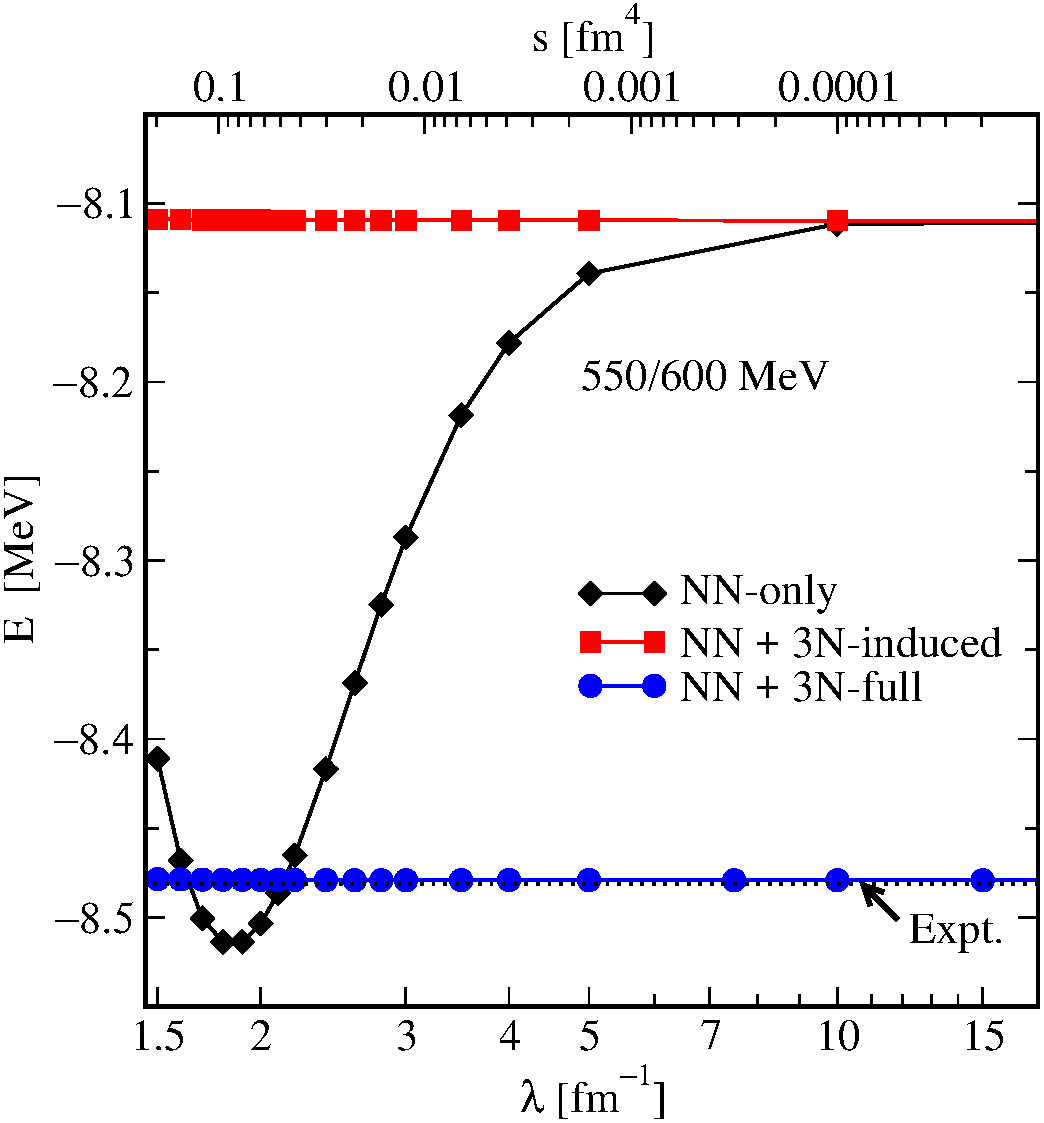
\includegraphics[width=0.55\unitlength,bb=10 10 560 560,clip]{\fdir/srg_evolution_energy.pdf}
  \end{center}  
  \vspace{-10pt}
  \caption{\label{fig:triton}Ground state energy of $\nuc{H}{3}$ as a function 
  of the flow parameter $\lambdaSRG$ for chiral \NNLO{} $NN$ and $NN\!+\!3N$ 
  interactions (see \cite{Hebeler:2012ly} for details). $NN$-only means initial and 
  induced $3N$ interactions are discarded, $NN\!+\!3N$-induced takes only 
  induced $3N$ interactions into account, and $3N$-full contains initial
  $3N$ interactions as well. The black dotted line shows the experimental 
  binding energy \cite{Wang:2012uq}. Data for the figure courtesy of 
  K.~Hebeler.}
\end{figure*}

Nowadays, state-of-the-art SRG evolutions of nuclear interactions are 
performed in the three-body system \cite{Jurgenson:2009bs,Jurgenson:2011zr,Jurgenson:2013fk, 
Hebeler:2012ly,Wendt:2013uq}. In figure \ref{fig:triton}, we show 
$\nuc{H}{3}$ ground-state energies that have been calculated with
a family of SRG-evolved interactions that is generated from a 
chiral \NNLO{} $NN$ interaction by Epelbaum, Gl\"ockle, and Mei\ss{}ner 
\cite{Epelbaum:2002nr,Epelbaum:2006mo},
and a matching $3N$ interaction (see \cite{Hebeler:2012ly} for
full details). As mentioned above, the SRG evolution is not unitary in 
the three-body system if we truncate the evolved interaction and
the SRG generator at the two-body level (\emph{N$N$-only}). The 
depends strongly on $\lambdaSRG$, varying by 5--6\% over the 
typical range that we consider here (cf.~section \ref{sec:srg_nn}). 
If we truncate the operators at the three-body level instead, induced 
$3N$ interactions are properly included and the unitarity of the 
transformation is restored (\emph{$NN\!+\!3N$-induced}): 
The energy does not change as $\lambdaSRG$ is varied. Finally, the 
curve \emph{$NN\!+\!3N$-full} shows results of calculations in
which a $3N$ force was included in the initial Hamiltonian and
evolved consistently to lower resolution scale as well. Naturally,
the triton ground-state energy is invariant under the SRG flow, and 
it closely reproduces the experimental value because the $3N$ interaction's 
low-energy constants are usually fit to give the correct experimental 
$\nuc{H}{3}$ ground-state energy (see, e.g., 
\cite{Epelbaum:2009ve,Machleidt:2011bh,Gazit:2009qf}).

Our example shows that it is important to track induced interactions,
especially when we want to use evolved nuclear Hamiltonians beyond
the few-body systems we have focused on here. The nature of the SRG 
as a continuous evolution works at least somewhat in our favor: As
discussed above, truncations of the SRG flow equations lead to a 
violation of unitarity that manifests as a (residual) dependence 
of our calculated few- and many-body observables on the resolution 
scale $\lambdaSRG$. We can use this dependence as a tool to assess 
the size of missing contributions, although one has to take great
care to disentangle them from the effects of many-body truncations,
unless one uses quasi-exact methods like the NCSM (see, e.g., 
\cite{Bogner:2010pq,Jurgenson:2009bs,Hebeler:2012ly,Roth:2011kx,Hergert:2013mi,Hergert:2013ij,Binder:2014fk,
Soma:2014eu,Griesshammer:2015dp}). If we want more detailed information,
then we cannot avoid to work with $3N, 4N, \ldots$ or higher many-nucleon 
forces. The empirical observation that SRG evolutions down to $\lambdaSRG\sim1.5\fmi$
appear to preserve the natural hierarchy of nuclear forces, i.e.,  
$NN > 3N > 4N > \ldots$, suggests that we can truncate induced
forces whose contributions would be smaller than the desired accuracy 
of our calculations. 

While we may not have to go all the way to the treatment of induced
$A-$nucleon operators, which would be as expensive as implementing 
the matrix flow in the $A-$body system (cf.~\ref{sec:srg_nn}),
dealing with induced $3N$ operators is already computationally 
expensive enough. Treating induced $4N$ forces explicitly is out 
of the question, except in schematic cases. However, there is a
way of accounting for effects of induced $3N,\ldots$ forces in
an implicit manner, by performing SRG evolutions in the nuclear
medium. 

%%%%%%%%%%%%%%%%%%%%%%%%%%%%%%%%%%%%%%%%%%%%%%%%%%%%%%%%%%%%%%%%%%%%%%
%%%%%%%%%%%%%%%%%%%%%%%%%%%%%%%%%%%%%%%%%%%%%%%%%%%%%%%%%%%%%%%%%%%%%%
% SECTION %%%%%%%%%%%%%%%%%%%%%%%%%%%%%%%%%%%%%%%%%%%%%%%%%%%%%%%%%%%%
%%%%%%%%%%%%%%%%%%%%%%%%%%%%%%%%%%%%%%%%%%%%%%%%%%%%%%%%%%%%%%%%%%%%%%
%%%%%%%%%%%%%%%%%%%%%%%%%%%%%%%%%%%%%%%%%%%%%%%%%%%%%%%%%%%%%%%%%%%%%%

\section{\label{sec:imsrg}The In-Medium SRG}
\tbd{[Bridge]}

%%%%%%%%%%%%%%%%%%%%%%%%%%%%%%%%%%%%%%%%%%%%%%%%%%%%%%%%%%%%%%%%%%%%%%
% SUBSECTION %%%%%%%%%%%%%%%%%%%%%%%%%%%%%%%%%%%%%%%%%%%%%%%%%%%%%%%%%
%%%%%%%%%%%%%%%%%%%%%%%%%%%%%%%%%%%%%%%%%%%%%%%%%%%%%%%%%%%%%%%%%%%%%%
\subsection{\label{sec:nord}Normal Ordering and Wick's Theorem}


%
% SUBSUBSECTION %%%%%%%%%%%%%%%%%%%%%%%%%%%%%%%%%%%%%%%%%%%%%%%%%%%%%%
%
\subsubsection{\label{sec:nord_ops}Normal-Ordered Operators}
To construct normal-ordered operators, we start from the usual Fermionic
creation and annihilation operators, $\aaO_i$ and $\aO_i$, which satisfy
the canonical anticommutation relations
\begin{equation}
  \acomm{\aaO_i}{\aaO_j} = \acomm{\aO_i}{\aO_j} = 0\,,\quad \acomm{\aaO_i}{\aO_j}=\delta_{ij}\,.
\end{equation}
The indices are collective labels for the quantum numbers of our single-particle 
states. Using the creators and annihilators, we can express any given $A$-body 
operator in second quantization. Moreover, we can construct a complete basis 
for a many-body Hilbert space by acting with products of $\aaO_i$ on the particle 
vacuum,
\begin{equation}\label{eq:vacbasis}
  \ket{\Phi\{i_1\ldots i_A\}}=\prod_{k=1}^A\aaO_{i_k}\ket{\text{vac}}\,,
\end{equation}
and letting the indices $i_1,\ldots,i_A$ run over all single-particle states.
The states $\ket{\Phi\{i_1\ldots i_A\}}$ are, of course, nothing but 
antisymmetrized product states, i.e., Slater determinants.

Of course, not all of the Slater determinants in our basis are created equal. 
We can usually find a Slater determinant that is a fair approximation 
to the nuclear ground state, and use it as a \emph{reference state} for the 
construction and organization of our many-body basis. By simple energetics, the 
ground state and low-lying excitation spectrum of an $A$-body nucleus are usually 
dominated by excitations of particles in the vicinity of the reference state's 
Fermi energy. This is especially true for $NN$ interactions that have
been evolved to a low resolution scale $\lambdaSRG$ (see section 
\ref{sec:srg_nn}). For such forces, the coupling between basis states whose
energy expectation values differ by much more than the characteristic energy 
$\hbar^2\lambda^2/m$ is suppressed. 

Slater determinants that are variationally optimized through a Hartree-Fock 
(HF) calculation have proven to be reasonable reference states for interactions 
with $\lambda\approx2.0\fm^{-1}$ (see, e.g., Refs.~\cite{Bogner:2010pq,Roth:2010vp,Barrett:2013oq,Hagen:2014ve,Hergert:2016jk,Tichai:2016vl} and references therein), allowing post-HF methods like MBPT, 
CC, or the IMSRG discussed below to converge rapidly to the exact result. 
Starting from such a HF reference state $\ket{\Phi}$, we can obtain 
a basis consisting of the state itself and up to $A$-particle, $A$-hole ($ApAh$) 
excitations:
\begin{equation}
  \ket{\Phi},\,\aaO_{p_1}\aO_{h_1}\ket{\Phi},\;\ldots\;,\,\aaO_{p_1}\ldots\aaO_{p_A}\aO_{h_A}\ldots\aO_{h_1}\ket{\Phi}\,.
\end{equation}
Here, indices $p_i$ and $h_i$ run over all one-body basis states with energies above 
(\emph{particle} states) and below the Fermi level (\emph{hole} states), respectively.
Such bases work best for systems with large gaps in the single-particle 
spectrum, e.g., closed-shell nuclei. If the gap is small, excited basis 
states can be nearly degenerate with the reference state, which usually 
results in spontaneous symmetry breaking and strong configuration mixing.

We can now introduce a one-body operator that is normal-ordered with respect
to the reference state $\ket{\Phi}$ by defining
\begin{equation}\label{eq:def_no}
  \aaO_i\aO_j \equiv \nord{\aaO_i\aO_j} +\, \contraction[1.5ex]{}{\aO}{{}^\dag_i}{\aO}\aaO_i\aO_j\,.
\end{equation}
The brace connecting a pair of creation and annihilation operators indicates
they have been \emph{contracted}. The contraction itself is merely the 
expectation value of the operator in the reference state $\ket{\Phi}$:
\begin{equation}\label{eq:def_particle_contraction}
  \contraction[1.5ex]{}{\aO}{{}^\dag_i}{\aO}\aaO_i\aO_j \equiv \matrixe{\Phi}{\aaO_i\aO_j}{\Phi} \equiv \rho_{ji} \,.
\end{equation}
By definition, the contractions are identical to the elements of the one-body 
density matrix of $\ket{\Phi}$ \cite{Ring:1980bb}. Starting from the one-body
case, we can define normal-ordered $A$-body operators recursively by evaluating 
all contractions between creation and annihilation operators, e.g., 
\begin{align}\label{eq:def_no_nbody}
   &\aaO_{i_1}\ldots\aaO_{i_A}\aO_{j_A}\ldots\aO_{j_1} \notag\\
    &\equiv\, \nord{\aaO_{i_1}\ldots\aaO_{i_A}\aO_{j_{A}}\ldots\aO_{j_{1}}} \notag\\
    &\hphantom{\equiv}
       + \contraction[1.5ex]{}{\aO}{{}^\dag_{i_1}}{\aO}\aaO_{i_1}\aO_{j_1} 
        \nord{\aaO_{i_2}\ldots\aaO_{i_A}\aO_{j_{A}}\ldots\aO_{j_{2}}} 
      -\; \contraction[1.5ex]{}{\aO}{{}^\dag_{i_1}}{\aO}\aaO_{i_1}\aO_{j_2} 
        \nord{\aaO_{i_2}\ldots\aaO_{i_A}\aO_{j_A}\ldots\aO_{j_{3}}\aO_{j_{1}}}
      + \text{\,singles}\notag\\
    &\hphantom{\equiv}
       + \left(
          \contraction[1.5ex]{}{\aO}{{}^\dag_{i_1}}{\aO}\aaO_{i_1}\aO_{j_1}
          \contraction[1.5ex]{}{\aO}{{}^\dag_{i_1}}{\aO}\aaO_{i_2}\aO_{j_2}
          -
          \contraction[1.5ex]{}{\aO}{{}^\dag_{i_1}}{\aO}\aaO_{i_1}\aO_{j_2}
          \contraction[1.5ex]{}{\aO}{{}^\dag_{i_1}}{\aO}\aaO_{i_2}\aO_{j_1}
        \right) 
        \nord{\aaO_{i_3}\ldots\aaO_{i_A}\aO_{j_A}\ldots\aO_{j_{3}}} + \text{\,doubles} \notag\\
    &\hphantom{\equiv}
  +\,\ldots\,+ \text{\,full contractions}\,.
\end{align}
Here, we have followed established quantum chemistry jargon (singles, doubles, 
etc.) for the number of contractions in a term (cf.~chapter \ref{chapter:cc}).
Note that the double contraction shown in the next-to-last line is identical
to the factorization formula for the two-body density matrix of a Slater 
determinant,
\begin{equation}
  \rho_{j_1j_2i_1i_2}
  \equiv
  \matrixe{\Phi}{\aaO_{i_1}\aaO_{i_2}\aO_{j_2}\aO_{j_1}}{\Phi}
  = \rho_{i_1j_1}\rho_{i_2j_2}- \rho_{i_1j_2}\rho_{i_2j_1}\,.
\end{equation}

From Eq.~\eqref{eq:def_no}, it is evident that $\matrixe{\Phi}{\nord{\aaO_i\aO_j}}{\Phi}$ 
must vanish, and this is readily generalized to expectation values of 
arbitrary normal-ordered operators in the reference state $\ket{\Phi}$,
\begin{equation}
  \matrixe{\Phi}{\nord{\aaO_{i_1}\ldots\aO_{i_1}}}{\Phi} = 0\,.
\end{equation}
This property of normal-ordered operators greatly facilitates calculations 
that require the evaluation of matrix elements in a space spanned by excitations 
of $\ket{\Phi}$. 

As an example, we consider an intrinsic nuclear $A$-body Hamiltonian 
containing both $NN$ and $3N$ interactions,
\begin{equation}\label{eq:def_Hint}
  H = \left(1-\frac{1}{\AO}\right)\TO^{[1]} + \frac{1}{\AO}\TO^{[2]} + \VO^{[2]} +\VO^{[3]}\,,
\end{equation}
where the one- and two-body kinetic energy terms are
\begin{align}
  \TO^{[1]} &\equiv \sum\frac{\pOV^2_i}{2m}\,,\\
  \TO^{[2]} &\equiv -\frac{1}{m}\sum_{i<j}\pOV_i\cdot\pOV_j
\end{align}
(see section \ref{sec:srg_nn} and \cite{Hergert:2009wh}). Choosing a 
single Slater determinant $\ket{\Phi}$ as the reference state, we can 
rewrite the Hamiltonian \emph{exactly} in terms of normal-ordered operators,
\begin{align}\label{eq:Hno}
  \HO &= E + \sum_{ij}f_{ij}\nord{\aaO_{i}\aO_{j}} + \frac{1}{4}\sum_{ijkl}\Gamma_{ijkl}\nord{\aaO_{i}\aaO_{j}\aO_{l}\aO_{k}}
    + \frac{1}{36}\sum_{ijklmn}W_{ijklmn}\nord{\aaO_{i}\aaO_{j}\aaO_{k}\aO_{n}\aO_{m}\aO_{l}}\,,
\end{align}
where the labels for the individual contributions have been chosen for 
historical reasons. For convenience, we will work in the eigenbasis of 
the one-body density matrix in the following, so that
\begin{equation}\label{eq:def_natorb}
  \rho_{ab}=n_{a}\delta_{ab}\,,\quad n_{a}\in\{0,1\}\,.
\end{equation}
The individual normal-ordered contributions in Eq.~\eqref{eq:Hno} are then 
given by
\begin{align}
  E &= \left(1-\frac{1}{A}\right)\sum_{a}\matrixe{a}{\tO^{[1]}}{a}n_{a}
      + \frac{1}{2}\sum_{ab}\matrixe{ab}{\frac{1}{A}\tO^{[2]}\!+\!\vO^{[2]}}{ab}n_{a}n_{b}
      + \frac{1}{6}\sum_{abc}\matrixe{abc}{\vO^{[3]}}{abc}n_{a}n_{b}n_{c}\,,\label{eq:E0}\\
%
  f_{ij} &= \left(1-\frac{1}{A}\right)\matrixe{i}{\tO^{[1]}}{j} 
      + \sum_{a}\matrixe{ia}{\frac{1}{A}\tO^{[2]}\!+\!\vO^{[2]}}{ja}n_{a}
      + \frac{1}{2}\sum_{ab}\matrixe{iab}{\vO^{[3]}}{jab}n_{a}n_{b}\,,\label{eq:f}   
      \\
% 
  \Gamma_{ijkl} &= \matrixe{ij}{\frac{1}{A}\tO^{(2)}\!+\!\vO^{[2]}}{kl} + \sum_{a}\matrixe{ija}{\vO^{[3]}}{kla}n_{a}\,,\label{eq:Gamma}\\
  W_{ijklmn}&=\matrixe{ijk}{\vO^{[3]}}{lmn}\,.
\end{align}
Due to the occupation number factors in Eqs.~\eqref{eq:E0}--\eqref{eq:Gamma}, the sums 
run only over states that are occupied in the reference state. This means that the 
zero-, one-, and two-body parts of the Hamiltonian all contain in-medium contributions 
from the free-space 3N interaction.

For low-momentum interactions, it has been shown empirically that the omission 
of the normal-ordered three-body piece of the Hamiltonian causes a deviation of merely 
1--2\% in ground-state and (absolute) excited state energies of light and medium-mass 
nuclei \cite{Hagen:2007zc,Roth:2011kx,Roth:2012qf,Binder:2013fk,Gebrerufael:2016fe}. 
This \emph{normal-ordered two-body approximation} (NO2B) to the Hamiltonian is
useful for practical calculations, because it provides an efficient means to 
account for $3N$ force effects in nuclear many-body calculations without incurring 
the computational expense of explicitly treating three-body operators. In section 
\ref{sec:imsrg_flow}, we will see that the NO2B approximation also meshes in a natural 
way with the framework of the IMSRG, which makes it especially appealing for our 
purposes.

%
% SUBSUBSECTION %%%%%%%%%%%%%%%%%%%%%%%%%%%%%%%%%%%%%%%%%%%%%%%%%%%%%%
%
\subsubsection{Wick's Theorem}
The normal-ordering formalism has additional benefits for the evaluation
of products of normal-ordered operators. Wick's theorem (see, e.g., \cite{Shavitt:2009}), 
which is a direct consequence of Eq.~\eqref{eq:def_no_nbody}, allows us to 
expand such products in the following way:
\begin{align}\label{eq:def_wick}
   & \nord{\aaO_{i_1}\ldots\aaO_{i_N}\aO_{j_{N}}\ldots\aO_{j_{1}}} 
     \nord{\aaO_{k_1}\ldots\aaO_{k_M}\aO_{l_{M}}\ldots\aO_{l_{1}}}
   \notag\\
    &=(-1)^{M\cdot N}  
     \nord{\aaO_{i_1}\ldots\aaO_{i_N}\aaO_{k_1}\ldots\aaO_{k_M}\aO_{j_{N}}\ldots\aO_{j_{1}}\aO_{l_{M}}\ldots\aO_{l_{1}}} 
    \notag\\
    &\hphantom{=}
       + (-1)^{M\cdot N}\contraction[1.5ex]{}{\aO}{{}^\dag_{i_1}}{\aO}\aaO_{i_1}\aO_{l_1} 
        \nord{\aaO_{i_2}\ldots\aaO_{k_M}\aO_{j_{N}}\ldots\aO_{l_{2}}} \notag\\
    &\hphantom{\equiv}
      + (-1)^{(M-1)(N-1)}\contraction[1.5ex]{}{\aO}{{}^\dag_{j_N}}{\aO}\aO_{j_N}\aaO_{k_1} 
        \nord{\aaO_{i_1}\ldots\aaO_{k_M}\aO_{j_{N}}\ldots\aO_{j_2}}
      \notag\\
    &\hphantom{=}
      + \text{\,singles}+ \text{\,doubles} + \ldots \,.
\end{align}
The phase factors appear because we anti-commute the creators and 
annihilators until they are grouped in the canonical order, i.e.,
all $\aaO$ appear to the left of the $\aO$. In the process, we also 
encounter a new type of contraction,
\begin{equation}\label{eq:def_hole_contraction}
  \contraction[1.5ex]{}{\aO}{{}^\dag_{i}}{\aO}\aO_{i}\aaO_{j} 
  \equiv \matrixe{\Phi}{\aO_{i}\aaO_{j}}{\Phi}
  = \delta_{ij} - \rho_{ij} \equiv \overline{\rho}_{ij}\,,
\end{equation}
as expected from the canonical anti-commutator algebra. $\overline\rho$
is the so-called \emph{hole density matrix}. 

The defining feature of Eq.~\eqref{eq:def_wick} is that only contractions 
between one index from each of the two strings of creation and annihilation
operators appear in the expansion, because contractions between indices 
within a single operator string have already been subtracted when we normal 
ordered it initially. In practical calculations, this leads to a substantial 
reduction of terms. An immediate consequence of Eq.~\eqref{eq:def_wick} is 
that a product of normal-ordered $M$ and $N$-body operators has the general 
form
\begin{equation}\label{eq:wick_product_schematic}
  \AO^{[M]}\BO^{[N]} = \sum_{k=|M-N|}^{M+N}\CO^{[k]}\,.
\end{equation}
Note that zero-body contributions, i.e., plain numbers, can only be generated 
if both operators have the same particle rank.

%%%%%%%%%%%%%%%%%%%%%%%%%%%%%%%%%%%%%%%%%%%%%%%%%%%%%%%%%%%%%%%%%%%%%%
% SUBSECTION %%%%%%%%%%%%%%%%%%%%%%%%%%%%%%%%%%%%%%%%%%%%%%%%%%%%%%%%%
%%%%%%%%%%%%%%%%%%%%%%%%%%%%%%%%%%%%%%%%%%%%%%%%%%%%%%%%%%%%%%%%%%%%%%
\subsection{\label{sec:imsrg_flow}In-Medium SRG Flow Equations}

%
% SUBSUBSECTION %%%%%%%%%%%%%%%%%%%%%%%%%%%%%%%%%%%%%%%%%%%%%%%%%%%%%%
%
\subsubsection{Induced Forces Revisited}
In section \ref{sec:srg_induced}, we discussed how SRG evolutions naturally
induce $3N$ and higher many-nucleon forces, because every evaluation of 
the commutator on the right-hand side of the operator flow equation 
\eqref{eq:opflow} increases the particle rank of $\HO(s)$, e.g.,
\begin{equation}\label{eq:induced_3N}
  \sum_{ijklpqrs}\eta_{ijkl}H_{pqrs}\comm{\aaO_{i}\aaO_{j}\aO_{l}\aO_{k}}{\aaO_{p}\aaO_{q}\aO_{s}\aO_{r}}
    = -\sum_{ijkqrs}\eta_{ijkl}H_{kqrs} \aaO_{i}\aaO_{j}\aaO_{q}\aO_{s}\aO_{r}\aO_{l} + \text{3N terms} + \text{2N terms}\,.
\end{equation}
Note that there are no induced $4N$ interactions, and that commutators
involving at least one one-body operator do not change the particle rank
(see problem \ref{problem:products}). In the free-space evolution, we 
found that the truncation of $3N$ forces in the flowing Hamiltonian caused
a significant flow-parameter dependence of observables in $A\geq 3$ systems.

Working in the medium and using normal-ordered operators, we can expand the 
induced $3N$ operators:
\begin{align}\label{eq:induced_3N_no}
  \sum_{ijkqrs}\eta_{ijkl}H_{kqrs} \aaO_{i}\aaO_{j}\aaO_{q}\aO_{s}\aO_{r}\aO_{l}
  =\sum_{ijkqrs}\eta_{ijkl}H_{kqrs} 
    \Big(&
      \nord{\aaO_{i}\aaO_{j}\aaO_{q}\aO_{s}\aO_{r}\aO_{l}} 
       + n_q\delta_{qs}\nord{\aaO_{i}\aaO_{j}\aO_{r}\aO_{l}} 
       + n_j n_q\delta_{jr}\delta_{qs}\nord{\aaO_{i}\aO_{l}} \notag\\
  &
       + n_in_j n_q\delta_{il}\delta_{jr}\delta_{qs}+ \text{perm.}\,.
    \Big)
\end{align}
If we now truncate operators to the normal-ordered two-body level, we keep
all the in-medium contributions of the induced $3N$ terms, and retain 
information that we would have lost in the free-space evolution. These
in-medium contributions continuously feed into the 0B, 1B, and 2B matrix 
elements of the flowing Hamiltonian as we integrate Eq.~\eqref{eq:opflow}.

%
% SUBSUBSECTION %%%%%%%%%%%%%%%%%%%%%%%%%%%%%%%%%%%%%%%%%%%%%%%%%%%%%%
%
\subsubsection{IM-SRG(2) Truncation}
The evolution of the Hamiltonian or any other observable by means of
the flow equation \eqref{eq:opflow} is a continuous unitary transformation
in $A-$nucleon space only if we keep up to induced $A$-nucleon 
forces. Because an explicit treatment of induced contributions up to the 
$A$-body level is simply not feasible, we have to introduce a truncation 
to close the system of flow equations.

As explained in the previous subsection, we can make such truncations 
more robust if we normal order all operators with respect to a reference
state that is a fair approximation to the ground state of our system
(or another exact eigenstate we might want to target). Here, we choose
to truncate operators at the two-body level, to avoid the computational
expense of treating explicit three-body operators. For low-momentum $NN+3N$
Hamiltonians, the empirical success of the NO2B approximation mentioned 
at the end of section \ref{sec:nord_ops} seems to support this truncation: 
The omission of the normal-ordered $3N$ term in exact calculations causes 
deviations of only $\sim1\%$ in the oxygen, calcium, and nickel isotopes
\cite{Roth:2012qf,Binder:2013fk,Binder:2014fk}.

Following this line of reasoning,  we demand that for all values of the
flow parameter $s$
\begin{align} 
  \etaO(s) &\approx\etaO^{(1)}(s)+\etaO^{(2)}(s)\,,\label{eq:imsrg2_eta}\\
  \HO(s) &\approx E(s) + f(s) + \Gamma(s)\,,\label{eq:imsrg2_H}\\
  \totd{}{s}\HO(s) &\approx \totd{}{s}E(s) + \totd{}{s}f(s) + \totd{}{s}\Gamma(s)\label{eq:imsrg2_dH}\,.
\end{align}
This is the so-called IMSRG(2) truncation, which has been our primary
workhorse in past applications 
\cite{Tsukiyama:2011uq,Tsukiyama:2012fk,Hergert:2013mi,Hergert:2013ij,Hergert:2014vn,Morris:2015ve,Hergert:2016jk}. It is the basis for all results that we will discuss in the remainder of this chapter. 
The IMSRG(2) is a cousin to Coupled Cluster with Singles and Doubles
(CCSD) and the ADC(3) scheme in Self-Consistent Green's Function Theory 
(see chapters \ref{chapter:cc} and \ref{chapter:scgf}). Since all three
methods (roughly) aim to describe the same type and level of many-body 
correlations, we expect to obtain similar results for observables.

Let us introduce the permutation symbol $P_{ij}$ to interchange the 
indices of any expression, i.e.,
\begin{equation}\label{eq:def_Pij}
  P_{ij} g(\ldots,i,\ldots,j) \equiv g(\ldots,j,\ldots,i)\,,
\end{equation}
Plugging equations \eqref{eq:imsrg2_eta}--\eqref{eq:imsrg2_dH} into 
the operator flow equation \eqref{eq:opflow} and evaluating the 
commutators with the expressions from the appendix, we obtain the 
following system of IMSRG(2) flow equations:
\begin{align}
  \totd{E}{s}&= \sum_{ab}(n_a-n_b)\eta_{ab} f_{ba} 
    + \frac{1}{2} \sum_{abcd}\eta_{abcd}\Gamma_{cdab} n_a n_b\bar{n}_c\bar{n}_d
    \label{eq:imsrg2_m0b}\,,\\[5pt]
% \end{align}
% 
% \begin{align}
  \totd{f_{12}}{s} &= 
  \sum_{a}(1+P_{12})\eta_{1a}f_{a2} +\sum_{ab}(n_a-n_b)(\eta_{ab}\Gamma_{b1a2}-f_{ab}\eta_{b1a2}) \notag\\ 
  &\quad +\frac{1}{2}\sum_{abc}(n_an_b\bar{n}_c+\bar{n}_a\bar{n}_bn_c) (1+P_{12})\eta_{c1ab}\Gamma_{abc2}
  \label{eq:imsrg2_m1b}\,,\\[5pt]
% \end{align}
% 
% \begin{align}
  \totd{\Gamma_{1234}}{s}&= 
  \sum_{a}\left\{ 
    (1-P_{12})(\eta_{1a}\Gamma_{a234}-f_{1a}\eta_{a234} )
    -(1-P_{34})(\eta_{a3}\Gamma_{12a4}-f_{a3}\eta_{12a4} )
    \right\}\notag \\
  &\quad+ \frac{1}{2}\sum_{ab}(1-n_a-n_b)(\eta_{12ab}\Gamma_{ab34}-\Gamma_{12ab}\eta_{ab34})
    \notag\\
  &\quad-\sum_{ab}(n_a-n_b) (1-P_{12})(1-P_{34})\eta_{b2a4}\Gamma_{a1b3}
    \label{eq:imsrg2_m2b}\,.
\end{align}
% \end{widetext}
Here, $\nn_i=1-n_i$, and the $s$-dependence has been suppressed for brevity. 
To obtain ground-state energies, we integrate Eqs.~\eqref{eq:imsrg2_m0b}--\eqref{eq:imsrg2_m2b} 
from $s=0$ to $s\to\infty$, starting from the initial components of the 
normal-ordered Hamiltonian (Eqs.~\eqref{eq:E0}--\eqref{eq:Gamma}).

%
% SUBSUBSECTION %%%%%%%%%%%%%%%%%%%%%%%%%%%%%%%%%%%%%%%%%%%%%%%%%%%%%%
%
\subsubsection{Diagrammatic Representation of the IMSRG(2) Flow Equations}

As we will discuss in more detail in Sec.~\ref{sec:mbpt}, 
Eqs.~\eqref{eq:imsrg2_m0b}--\eqref{eq:imsrg2_m2b} can easily be translated 
into Goldstone or Hugenholtz diagrams for the flowing Hamiltonian $H(s)$.
This provides us with an intuitive understanding of the mechanism through
which the IM-SRG is non-perturbatively re-summing the many-body expansion. The second
and third rows of Eq.~\eqref{eq:imsrg2_m2b}, in particular, re-sum $pp/hh$-ladder and $ph$-ring 
diagrams, respectively. Due to the use of $H(s)$, ladder-ring interference 
diagrams are generated in the limit $s\to\infty$, and therefore the IM-SRG(2) 
goes beyond the more traditional Brueckner $G$-matrix or Random-Phase 
Approximation-type summations \cite{Day:1967zl,Brandow:1967tg,Fetter:2003ve}. 
Furthermore, the commutator structure of Eq.~\eqref{eq:opflow} ensures that 
the IM-SRG is size-extensive, and only connected diagrams are generated and
re-summed by the IM-SRG flow \cite{Brandow:1967tg,Shavitt:2009}. This property
is preserved even if the commutators are truncated at a given operator rank, as in the IM-SRG(2) case presented here. 



%
% SUBSUBSECTION %%%%%%%%%%%%%%%%%%%%%%%%%%%%%%%%%%%%%%%%%%%%%%%%%%%%%%
%
\subsubsection{Computational Scaling}
Let us briefly consider the computational scaling of the IMSRG(2) scheme,
ahead of the discussion of an actual implementation in section \ref{sec:imsrg_implementation}.
When performing a single integration step, the computational effort is 
dominated by the two-body flow equation \eqref{eq:imsrg2_m2b}, which 
naively requires $\OC(N^6)$ operations, where $N$ denotes the size of
the single-particle basis. This puts the IMSRG(2) in the same category 
CCSD and ADC(3) (see chapters \ref{chapter:cc} and \ref{chapter:scgf}).
Fortunately, large portions of the flow equations can be expressed in 
terms of matrix products, allowing us to use optimized linear algebra 
libraries provided by high-performance computing vendors. 

Moreover, we can further reduce the computational cost by distinguishing 
particle and hole states, because the number of hole states $N_h$ is 
typically much smaller than the number of particle states $N_p\sim N$. 
The best scaling we can achieve in the IMSRG(2) depends on the choice of 
generator (see section \ref{sec:imsrg_generator}). If the one- and two-body parts of the 
generator only consist of $ph$ and $pphhh$ type matrix elements and their 
Hermitian conjugates, the scaling is reduced to $\OC(N_h^2N_p^4)$, 
which matches the cost of solving the CCSD amplitude equations.



%%%%%%%%%%%%%%%%%%%%%%%%%%%%%%%%%%%%%%%%%%%%%%%%%%%%%%%%%%%%%%%%%%%%%%
% SUBSECTION %%%%%%%%%%%%%%%%%%%%%%%%%%%%%%%%%%%%%%%%%%%%%%%%%%%%%%%%%
%%%%%%%%%%%%%%%%%%%%%%%%%%%%%%%%%%%%%%%%%%%%%%%%%%%%%%%%%%%%%%%%%%%%%%
\subsection{Fluffy}
Naively, one could try to solve the flow equation \eqref{eq:flowEquations} by
choosing a suitable basis of the many-body Hilbert space and turning
Eq.~\eqref{eq:flowEquations} into a matrix differential equation, but such an
approach would ultimately amount to a diagonalization of the many-body
Hamiltonian. To make matters worse, implementing the flow means we
would deal with the Hamiltonian's full spectrum rather than just some
extremal eigenvalues that can be extracted efficiently in
state-of-the-art, large-scale large scale diagonalization approaches based on iterative techniques
\cite{Golub:2013le}.



Instead of performing SRG in free space, the evolution can be done at
finite density, that is directly in the $A$-body system
\cite{Kehrein:2006kx}. This approach has recently been applied very
successfully in nuclear physics, see the recent review of Bogner, Hergert, Morris and collaborators 
\cite{Hergert:2016jk,Hergert:2016ng,Morris:2016xp},
and is called in-medium SRG (IM-SRG). The method allows the evolution
of $3,...,A$-body operators using only two-body machinery, with the
simplifications arising from the use of normal-ordering with respect
to a reference state.

In our case, we assume that the problem can be modelled by a
Hamiltonian containing maximally two-body interaction, as done in chapters 8 and 9. In
second-quantized form, we defined in chapter 8 the normal-ordered Hamiltonian as
\[
\hat{H}_N = \sum_{pq} \langle p|\hat{h}_0|q\rangle a^\dagger_p
a_q+\frac{1}{4} \sum_{pqrs} \langle pq|\hat{v}|rs\rangle a^\dagger_p a^\dagger_q a_s a_r+\sum_{pq,i\le F}
\langle pi|\hat{v}|qi\rangle a^\dagger_p a_q.
\]
In chapter 8 we rewrote the normal-ordered Hamiltonian 
in terms of a new one-body operator and a two-body operator
\[
\hat{H}_N=\hat{F}_N+\hat{V}_N,
\]
with
\[
\hat{F}_N=\sum_{pq} \langle p|\hat{f}|q\rangle a^\dagger_pa_q,
\]
where
\[
\langle p|\hat{f}|q\rangle= \langle p|\hat{h}_0|q\rangle +\sum_{i\le F}
\langle pi|\hat{v}|qi\rangle.
\]
The last term on the right hand side represents a medium modification
to the single-particle Hamiltonian due to the two-body interaction.
Finally, the two-body interaction is given by
\[
\hat{V}_N = \frac{1}{4} \sum_{pqrs} \langle pq|\hat{v}|rs\rangle a^\dagger_p a^\dagger_q a_s a_r.
\]
In the equations below we will use the following shorthand notation for the matrix elements
\[
f_{pq}=\langle p|\hat{f}|q\rangle,
\]
and 
\[
v_{pqrs}= \langle pq|\hat{v}|rs\rangle.
\]
As discussed in chapter 8, the indices $i,j,k,...$
denote hole states below the Fermi level, indices $a,b,c,...$
particles states above the Fermi level, and indices $ p,q,r,...$ can
be used for both particle and hole states. As reference state
$|\Phi_0\rangle$ we choose the ground state of the non-interacting
system, where all single-particle orbitals below the Fermi level are
occupied.

Integrating the flow equations~(\ref{eq:flowEquations}), we face one
of the major challenges of the SRG method, namely the generation of
higher and higher order interaction terms during the flow. With each
evaluation of the commutator, the Hamiltonian gains terms of higher
order, and these induced contributions will in subsequent integration
steps contribute to terms of lower order. In principle, this continues
to infinity. 
To make the method computationally possible, we have to
close the IM-SRG flow equations, suggesting that we are forced to
truncate the equations to a certain order. We choose to truncate both
$\hat{H}_s$ and $\hat{\eta}_s$ at the two-body level, an approach
which is referred to as IM-SRG(2).  This normal-ordered two-body
approximation seems to be sufficient in many cases and has yielded
excellent results for several nuclei
\cite{Tsukiyama:2011uq,Tsukiyama:2012fk,Hergert:2016jk,Hergert:2016ng}.

The
commutator in the flow equations (\ref{eq:flowEquations}) guarantees
that the IM-SRG wave function $U_s^\dagger|\Phi\rangle$ can be
expanded in terms of linked diagrams only
\cite{Shavitt:2009,Hergert:2016jk,Hergert:2016ng}, which suggests that IM-SRG
is size-extensive. Regarding the quality of the SRG results, it means
that the error introduced by truncating the many-body expansions
scales linearly with the number of particles~$N$.

With this
truncation, the generator $\hat{\eta}$ can be written as
\[
\hat{\eta} = \sum_{pq} \eta_{pq}^{(1)} a_p^{\dagger}a_q  +
\frac{1}{4}\sum\limits_{pqrs}\eta_{pqrs}^{(2)} a_p^{\dagger}a_q^{\dagger}a_s
a_r,
\]
where $\eta_{pq}^{(1)}$ and $ \eta_{pqrs}^{(2)}$ are the one- and
two-body elements, respectively. Making use of the permutation
operator $ \hat{P}_{pq}f(p,q) = f(q,p)$ defined in chapter 8, the IM-SRG(2) flow equations
are given by
\begin{align}
\frac{d E_0}{ds} &= \sum_{ia}\left( \eta_{ia}^{(1)}f_{ai} -
\eta_{ai}^{(1)}f_{ia}\right) +
\frac{1}{2}\sum_{ijab}\eta_{ijab}^{(2)}v_{abij},
\label{eq:flow1}\\
\frac{d f_{pq}}{ds}&= \sum_r \left(\eta_{pr}^{(1)}f_{rq} +
\eta_{qr}^{(1)}f_{rp}\right) + \sum_{ia}\left(1-\hat{P}_{ia}\right)\left(
\eta_{ia}^{(1)}v_{apiq} - f_{ia}\eta_{apiq}^{(2)} \right)\notag \\ &
+\frac{1}{2} \sum_{aij} \left(1+\hat{P}_{pq}\right)
\eta_{apij}^{(2)}v_{ijaq} + \frac{1}{2}\sum_{abi}\left(1+\hat{P}_{pq}\right) \eta_{ipab}^{(2)}v_{abiq},
\label{eq:flow2}
\end{align}
\begin{align}
\frac{d v_{pqrs}}{ds} &= \sum_t \left(1-\hat{P}_{pq} \right)\left(
\eta_{pt}^{(1)}v_{tqrs}-f_{pt}\eta_{tqrs}^{(2)}\right)-\sum_t \left(
1-\hat{P}_{rs} \right)\left(\eta_{tr}^{(1)} v_{pqts} - f_{tr}
\eta_{pqts}^{(2)}\right)\notag \\ & +\frac{1}{2}\sum_{ab}
\left(\eta_{pqab}^{(2)} v_{abrs} - v_{pqab}\eta_{abrs}^{(2)}\right)-
\frac{1}{2}\sum_{ij} \left(\eta_{pqij}^{(2)} v_{ijrs} -
v_{pqij}\eta_{ijrs}^{(2)}\right)\notag \\ & -\sum_{ia} \left(1-
\hat{P}_{ia} \right)\left(1-\hat{P}_{pq}\right)\left(1-\hat{P}_{rs} \right)
\eta_{aqis}^{(2)}v_{ipar}.
\label{eq:flow3}
\end{align}
Note that for brevity, we have skipped the explicit $s$-dependence in the equations.

%%%%%%%%%%%%%%%%%%%%%%%%%%%%%%%%%%%%%%%%%%%%%%%%%%%%%%%%%%%%%%%%%%%%%%
% SUBSECTION %%%%%%%%%%%%%%%%%%%%%%%%%%%%%%%%%%%%%%%%%%%%%%%%%%%%%%%%%
%%%%%%%%%%%%%%%%%%%%%%%%%%%%%%%%%%%%%%%%%%%%%%%%%%%%%%%%%%%%%%%%%%%%%%
\subsection{\label{sec:imsrg_decoupling}Decoupling}


%%%%%%%%%%%%%%%%%%%%%%%%%%%%%%%%%%%%%%%%%%%%%%%%%%%%%%%%%%%%%%%%%%%%%%
% SUBSECTION %%%%%%%%%%%%%%%%%%%%%%%%%%%%%%%%%%%%%%%%%%%%%%%%%%%%%%%%%
%%%%%%%%%%%%%%%%%%%%%%%%%%%%%%%%%%%%%%%%%%%%%%%%%%%%%%%%%%%%%%%%%%%%%%
\subsection{\label{sec:imsrg_generator}Choice of Generator}
To determine the specific unitary transformation, one needs to specify
the generator~$\hat{\eta}$. Through different choices, the SRG flow
can be adapted to the features of a particular problem.\\

%
% SUBSUBSECTION %%%%%%%%%%%%%%%%%%%%%%%%%%%%%%%%%%%%%%%%%%%%%%%%%%%%%%
%
\subsubsection{Wegner's canonical generator}
The original choice, suggested by Wegner \cite{Wegner:1994dk}, reads
\begin{equation} 
\hat{\eta} = \left[ \hat{H}^{\rm d}, \hat{H}^{\rm od} \right] = \left[ \hat{H}^{\rm d}, \hat{H}
  \right].
\label{eq:etaWegner}
\end{equation} 
As commutator between two Hermitian operators, $\hat{\eta}$
fulfils the criterion of antihermiticity and can be shown to suppress
the off-diagonal matrix elements \cite{Kehrein:2006kx}. In general,
matrix elements far off the diagonal, where the Hamiltonian connects
states with large energy differences, are suppressed much faster than
elements closer to the diagonal. 

Evaluating the commutator, we get
for the one- and two-body elements
\begin{align*}
\eta_{pq}^{(1)} = & \sum_{r}\left(f_{pr}^d f_{rq} - f_{pr} f_{rq}^d \right)
+ f_{pq} v_{qppq}^d \left(n_q - n_p \right)\\ \eta_{pqrs}^{(2)} = & -
\sum_t \left[ \left(1-\hat{P}_{pq} \right)f_{pt} v_{tqrs}^d - \left(1 -
\hat{P}_{rs} \right)f_{tr} v_{pqts}^d \right] \notag \\ & + \sum_t
\left[  \left(1 - \hat{P}_{pq} \right)f_{pt}^d v_{tqrs} - \left(1 -
\hat{P}_{rs} \right)f_{tr}^d v_{pqts} \right]  \notag \\ & +
\frac{1}{2} \sum_{tu} (1 - n_t - n_u) \left(v_{pqtu}^d v_{turs} -
v_{pqtu} v_{turs}^d \right)\notag \\ & + \sum_{tu} \left(n_t - n_u \right)\left(
1 - \hat{P}_{pq} \right)\left(1 - \hat{P}_{rs} \right)v_{tpur}^d v_{uqts},
\end{align*}
where we use the standard notation
\[
n_p = \begin{cases} 1, & \mbox{if } p< \epsilon_F \quad(p\;\mbox{is
    hole state})\\ 0, &\mbox{if } p> \epsilon_F \quad(p\;\mbox{is
    particle state})\\
\end{cases}.
\]

%
% SUBSUBSECTION %%%%%%%%%%%%%%%%%%%%%%%%%%%%%%%%%%%%%%%%%%%%%%%%%%%%%%
%
\subsubsection{White's generator}
Apart from this canonical generator, there exist several other ones in
literature. One of them is White's choice
\cite{White:2002fk}, which makes numerical approaches much
more efficient.  The problem with Wegner's generator are the widely
varying decaying speeds of the elements, removing first terms with
large energy differences and then subsequently those ones with smaller
energy separations.  That way the flow equations become a stiff set of
coupled differential equations, which often gets numerically
unstable.\\ White takes an alternative approach, which is especially
suited for problems where one is interested in the ground state of a
system. Instead of driving all off-diagonal elements of the
Hamiltonian to zero, he focuses solely on those ones that are
connected to the reference state $|\Phi_0\rangle$, aiming to decouple
the reference state from the remaining Hamiltonian. With a suitable
transformation, the elements get similar decaying speeds, which solves
the problem of stiffness of the flow equations.  The generator is
explicitly constructed the following way \cite{White:2002fk}
\begin{align}
\hat{\eta} &= \sum_{ai} \frac{f_{ai}}{f_a-f_i-v_{aiai}}\lbrace a_a^{\dagger}a_i\rbrace -\text{hc} \notag \\ & + \sum_{abij}
\frac{v_{abij}}{f_a+f_b-f_i-f_j+A_{abij}}\lbrace a_a^{\dagger}a_b^{\dagger}a_j
a_i\rbrace - \text{hc},
\label{eq:WhiteFull}
\end{align}
with $f_p \equiv f_{pp}$, 'hc' denoting the Hermitian conjugate, and
\[
A_{abij} = v_{abab} + v_{ijij} - v_{aiai} - v_{ajaj} - v_{bibi} -
v_{bjbj}.
\label{eq:White7}
\]
Compared to Wegner's canonical generator, where the final flow
equations involve third order powers of the $f$- and $v$-elements,
these elements contribute only linearly with White's generator, which
results in much better numerical properties.


{\bf add more? Magnus discussion ? derivation of the equations?}


% \begin{table}[t]
%   \begin{center}
%       \begin{tabular}{| l | l | l | l | l |}
%       \hline State Label & p & 2s$_z$ & E & type\\ \hline 
%       0 & 1 &  1 & -g/2  & hole \\ 
%       1 & 1 & -1 & -g/2  & hole \\ 
%       2 & 2 &  1 & 1-g/2 & hole \\ 
%       3 & 2 & -1 & 1-g/2 & hole \\ 
%       4 & 3 & 1 & 2 & particle \\ 
%       5 & 3 & -1 & 2 & particle \\ 
%       6 & 4 & 1 & 3 & particle \\ 
%       7 & 4 & -1 & 3 & particle \\ \hline
%       \end{tabular}
%   \end{center}
%   \caption{\label{tab:imsrg_pairing_reference}Single-particle states and their quantum numbers and their energies from Eq.~(\ref{eq:pairingsp}). The degeneracy for every quantum number $p$ is equal to 2 due to the two possible spin values.} 
% \end{table}


%%%%%%%%%%%%%%%%%%%%%%%%%%%%%%%%%%%%%%%%%%%%%%%%%%%%%%%%%%%%%%%%%%%%%%
% SUBSECTION %%%%%%%%%%%%%%%%%%%%%%%%%%%%%%%%%%%%%%%%%%%%%%%%%%%%%%%%%
%%%%%%%%%%%%%%%%%%%%%%%%%%%%%%%%%%%%%%%%%%%%%%%%%%%%%%%%%%%%%%%%%%%%%%
\subsection{\label{sec:imsrg_implementation}Implementation}

%%%%%%%%%%%%%%%%%%%%%%%%%%%%%%%%%%%%%%%%%%%%%%%%%%%%%%%%%%%%%%%%%%%%%%
% SUBSECTION %%%%%%%%%%%%%%%%%%%%%%%%%%%%%%%%%%%%%%%%%%%%%%%%%%%%%%%%%
%%%%%%%%%%%%%%%%%%%%%%%%%%%%%%%%%%%%%%%%%%%%%%%%%%%%%%%%%%%%%%%%%%%%%%
\subsection{The Pairing Hamiltonian}

%%%%%%%%%%%%%%%%%%%%%%%%%%%%%%%%%%%%%%%%%%%%%%%%%%%%%%%%%%%%%%%%%%%%%%
% SUBSECTION %%%%%%%%%%%%%%%%%%%%%%%%%%%%%%%%%%%%%%%%%%%%%%%%%%%%%%%%%
%%%%%%%%%%%%%%%%%%%%%%%%%%%%%%%%%%%%%%%%%%%%%%%%%%%%%%%%%%%%%%%%%%%%%%
%%%%%%%%%%%%%%%%%%%%%%%%%%%%%%%%%%%%%%%%%%%%%%%%%%%%%%%%%%%%%%%%%%%%%%
\subsection{Infinite Neutron Matter}

%%%%%%%%%%%%%%%%%%%%%%%%%%%%%%%%%%%%%%%%%%%%%%%%%%%%%%%%%%%%%%%%%%%%%%
%%%%%%%%%%%%%%%%%%%%%%%%%%%%%%%%%%%%%%%%%%%%%%%%%%%%%%%%%%%%%%%%%%%%%%
% SECTION %%%%%%%%%%%%%%%%%%%%%%%%%%%%%%%%%%%%%%%%%%%%%%%%%%%%%%%%%%%
%%%%%%%%%%%%%%%%%%%%%%%%%%%%%%%%%%%%%%%%%%%%%%%%%%%%%%%%%%%%%%%%%%%%%%
%%%%%%%%%%%%%%%%%%%%%%%%%%%%%%%%%%%%%%%%%%%%%%%%%%%%%%%%%%%%%%%%%%%%%%

\section{\label{sec:perspectives}Conclusions and Perspectives}
\begin{itemize}
\item Magnus
\item Multi-reference
\item TVS-IMSRG
\end{itemize}


In this work, we have presented a comprehensive review of the IM-SRG
as a powerful \emph{ab initio} method for nuclei. The IM-SRG employs
the flow-equation formulation of the SRG to decouple an $A$-body
reference state from particle-hole excitations, thus solving the
many-body Schr\"odinger equation. Compared to other \emph{ab initio}
approaches for medium-mass nuclei, we have shown that the IM-SRG is
competitive with CC and SCGF calculations, both in terms of accuracy and of
computational efficiency.

In the IM-SRG, the Hamiltonian is normal ordered with respect to the
reference state and typically truncated at the normal-ordered two-body
level. In this way, 3N interactions can be naturally included in a
normal-ordered two-body approximation. Due to the many ongoing
developments of 3N forces, we have focused in this review on a
detailed derivation at the NN level, but discuss highlights of first
IM-SRG calculation including 3N interactions in Sec.~\ref{sec:3N}.

Going beyond the closed-shell or single-reference version, the IM-SRG
has been recently generalized to a multi-reference formulation, as
discussed in Sec.~\ref{sec:mrimsrg}. The multi-reference IM-SRG (MR-IM-SRG) is
based on a generalized version of normal-ordering and Wick's
theorem. In principle, one can use 
arbitrary reference states that are
characterized by one-, two- and three-body density matrices. In the
first multi-reference applications, particle-number-projected
Hartree-Fock-Bogoliubov states were used as reference states for
describing the even nuclei throughout semi-magic isotopic chains.

A great asset of the IM-SRG is the flexibility and simplicity of its
basic concept. Through different choices of generators and decoupling
patterns, the numerical characteristics and efficiency of the methods
can be controlled and tailored for specific applications. The
in-medium evolved Hamiltonian is directly accessible, Hermitian and readily
usable for subsequent nuclear structure calculations.

As a specific application that exploits this flexibility,
nonperturabtive derivations of valence-space Hamiltonians have been
achieved. In the IM-SRG for open-shell nuclei, states with $A_v$
particles in the valence space are additionally decoupled from those
containing non-valence admixtures. This gives the energy of the
closed-shell core (as in the standard IM-SRG), but also valence-space
single-particle energies and residual interactions. The resulting
valence-space Hamiltonian can then be diagonalized using large-scale
shell-model methods. The IM-SRG provides for the first time a
nonperturbative derivation of effective interactions in the shell
model based on nuclear forces without adjustments. This is discussed
in Sec.~\ref{sec:shell_model}.

Finally, we highlight novel technical advances of the Magnus expansion
for effective operators in Sec.~\ref{sec:magnus}. This enables a
consistent evolution of operators in the IM-SRG for applications to
nuclear structure, electroweak transitions, and for key matrix elements
needed for fundamental symmetry tests.

%%%%%%%%%%%%%%%%%%%%%%%%%%%%%%%%%%%%%%%%%%%%%%%%%%%%%%%%%%%%%%%%%%%%%%
% SUBSECTION %%%%%%%%%%%%%%%%%%%%%%%%%%%%%%%%%%%%%%%%%%%%%%%%%%%%%%%%%
%%%%%%%%%%%%%%%%%%%%%%%%%%%%%%%%%%%%%%%%%%%%%%%%%%%%%%%%%%%%%%%%%%%%%%
\subsection{Technical Advances: Magnus Expansion and Effective Operators}
\label{sec:magnus}

\begin{figure}[t]
\begin{center}
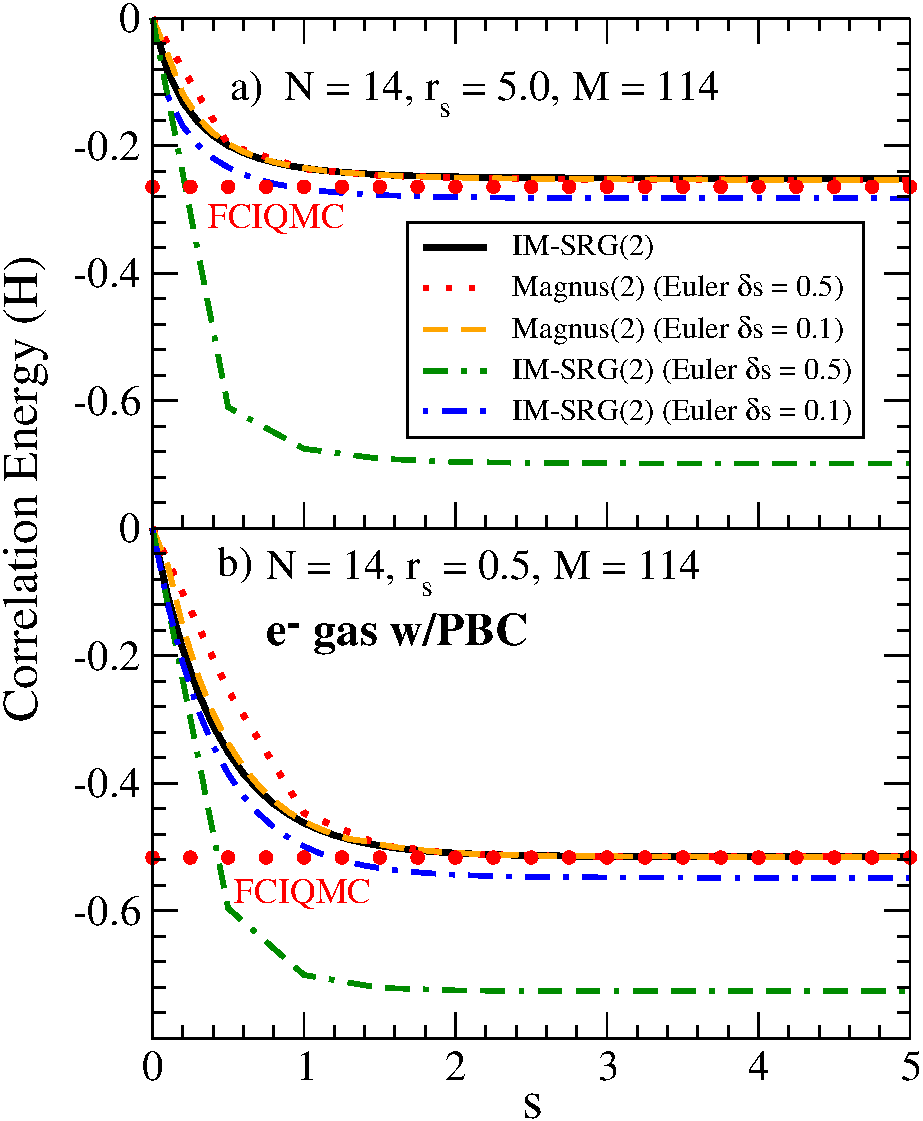
\includegraphics[width=.6\columnwidth]{\fdir/HEG_diffstepsizes}
\caption{\label{fig:timestep_HEG}
(Color online) Flowing IM-SRG(2) and Magnus(2) correlation energy for 
the electron gas, $E_0(s)-E_{\rm HF}$, for Wigner-Seitz radii of a)
$r_s=5.0$ and b) $r_s=0.5$. The solid black line corresponds to the
IM-SRG(2) results using an adaptive solver based on the
Adams-Bashforth method, while the other lines correspond to Magnus(2)
and IM-SRG(2) results using different Euler step sizes. The red
circles denote the quasi-exact FCIQMC results of
Ref.~\cite{Shepherd:2012hl}.}
\end{center}
\end{figure}

Despite modest computational scaling and the flexibility to tailor the
generator to different systems, IM-SRG calculations based on the
direct integration of Eqs.~(\ref{eq:opflow}) and~(\ref{eq:obsflow}) are
limited by the memory demands of the ODE solver. The use of a
high-order solver is essential, as the accumulation of time-step
errors destroys the unitary equivalence between $H(s)$ and $H(0)$ even
if no truncations are made in the flow equations. State-of-the-art
solvers can require the storage of 15-20 copies of the solution vector
in memory, which is the main computational bottleneck of the method.
What is worse, the dimensionality of the flow equations roughly
doubles for each additional observable one wishes to calculate, and
each operator can evolve with rather different timescales than the
Hamiltonian, increasing the likelihood of the ODEs becoming
stiff.

\begin{figure}[t]
\begin{center}
\includegraphics[width=.6\columnwidth]{\fdir/O16_diffstepsizes}
\caption{\label{fig:timestep_O16}
(Color online) Flowing IM-SRG(2) and Magnus(2) ground-state energy, 
$E_0(s)$, for $^{16}$O starting from the N$^3$LO NN interaction of
Entem and Machleidt~\cite{Entem:2003th,Machleidt:2011bh} evolved by
the free-space SRG to a) $\lambda=2.7$ fm$^{-1}$ and $\lambda = 2.0$
fm$^{-1}$. The solid black line corresponds to IM-SRG(2) results using
an adaptive solver based on the Adams-Bashforth method, while the
other lines correspond to Magnus(2) and IM-SRG(2) results using
different Euler step sizes. The calculations were done in an
$e_{max}=8$ model space, with $\hbar\omega = 24$~MeV for the
underlying harmonic-oscillator basis.}
\end{center}
\end{figure}

To bypass these limitations, an improved formulation of the IM-SRG was
proposed in Ref.~\cite{Morris:2015ve} that utilizes the Magnus
expansion from the theory of matrix differential
equations~\cite{Magnus:1954xy,Blanes:2009fk}.  In essence, the problem
is recast so that rather than solving flow equations for the
Hamiltonian and other operators of interest, one solves flow equations
for the anti-Hermitian operator $\Omega(s)$, where $U(s) =
e^{\Omega(s)}$. The unitary operator $U(s)$ is then used to transform
the Hamiltonian and any other operators of interest via the
Baker-Cambell-Hausdorff (BCH) formula. The advantage of the Magnus
formulation stems from the fact that the flow equations for
$\Omega(s)$ can be solved using a simple first-order Euler step method
without any loss of accuracy, resulting in substantial memory savings
and a modest reduction in CPU time.  In the conventional approach,
time-step errors accumulate directly in the evolved $H(s)$,
necessitating the use of a high-order solver to preserve an acceptable
level of accuracy.  In the Magnus formulation, even though sizable
time-step errors accumulate in $\Omega(s)$ with a first-order method, 
upon exponentiation the transformation is still unitary, and
the transformed $H(s)=\UO(s)H\UUO(s)$ is unitarily equivalent to
the initial Hamiltonian modulo any truncations made in evaluating the BCH formula.  For
further details on the implementation of the Magnus formulation, see
Ref.~\cite{Morris:2015ve}.

The insensitivity to time-step errors is illustrated in
Figs.~\ref{fig:timestep_HEG} and~\ref{fig:timestep_O16}, which show
the 0-body part of the flowing Hamiltonian $H(s)$ versus the flow
parameter for the electron gas, where we plot $E_0(s)-E_\text{HF}$ as an
approximation of the correlation energy at large $s$, and for
$^{16}$O, respectively. The black solid lines denote the results of a
standard IM-SRG(2) calculation using the predictor-corrector solver of
Shampine and Gordon, while the other curves denote IM-SRG(2) and
Magnus(2) calculations using a first-order Euler method with different
step sizes $\delta s$. For the electron gas, the exact full
configuration quantum Monte Carlo (FCIQMC)
results~\cite{Shepherd:2012hl} are shown for
reference. Unsurprisingly, the IM-SRG(2) calculations using a
first-order Euler method are very poor, with the various step sizes
converging to different large-$s$ limits. The Magnus(2) calculations,
on the other hand, converge to the same large-$s$ limit in excellent
agreement with the standard IM-SRG(2) and the FCIQMC results.

The evaluation of general operators poses considerable computational
challenges in the conventional formulation of the IM-SRG. In the
Magnus expansion formulation, the evolution of additional operators is
relatively straightforward since the dimensionality of the flow
equations is fixed, regardless of how many additional operators are
being evolved. Proof-of-principle operator evolutions have been
carried out for for the momentum distribution in the electron gas, and
the generalized center-of-mass Hamiltonian in $^{16}$O with encouraging
results~\cite{Morris:2015ve}.  The relative ease of performing
operator evolution is especially encouraging for shell model
applications, as it opens up the exciting possibility for consistent,
nonperturbative calculations of both Shell-Model Hamiltonians and
effective electroweak operators (e.g., the $0\nu\beta\beta$ matrix
element, quenching of Gamow-Teller strength, etc.) relevant for
studies of fundamental symmetries in nuclei.


% \subsection{Medium-Mass Nuclei with Three-Nucleon Forces}
% \label{sec:3N}

% \begin{figure}[t]
%   \setlength{\unitlength}{0.8\textwidth}
%   \begin{picture}(1.0000,0.800)
%     \put(-0.0500,0.3200){\small\input{fig/chi2b3bi_srgXXXX_Eint.tex}}
%     \put(-0.0500,0.0000){\small\input{fig/chi2b3b400_srgXXXX_Eint.tex}}
%   \put(1.0000,0.5200){\parbox{0.1600\unitlength}{
%     \framebox{
%     \begin{tabular*}{0.16\unitlength}{l@{\extracolsep\fill}l}
%          \multicolumn{2}{c}{\footnotesize $\lambda[\fmi]$} \\
%          \scriptsize\symbolcircle[FGBlue]     & \footnotesize2.24 \\
%          \scriptsize\symbolbox[FGRed]         & \footnotesize2.00 \\
%          \scriptsize\symboldiamond[FGGreen]   & \footnotesize1.88 \\
%          \scriptsize\symboltriangle[FGOrange] & \footnotesize$\infty$
%     \end{tabular*}
%     }
%     }
%   }
%   \end{picture}
%   \vspace{-30pt}
%   \caption{\label{fig:chi2b3bXXXX_srgXXXX_Eint}
%     IM-SRG(2) ground-state energies per nucleon for light and medium-mass closed-shell isotopes from chiral NN and NN+3N interactions at different resolution scales $\lambda$ (see text). Experimental values (black bars) taken from \cite{Wang:2012uq}. \emph{Top panel:} Bare \NNNLO at $\lambda=\infty$, and \NNNLO plus induced 3N interactions for $\lambda<\infty$. \emph{Bottom panel:} \NNNLO NN plus local \NNLO interaction with initial cutoff $\LambdaNNN=400\,\MeV$, evolved to lower resolution scale.
%   }
% \end{figure}

% For most of the present work, we have focused on bare or softened
% chiral NN interactions only for the sake of simplicity. Key aspects of
% the IM-SRG, like the convergence behavior of ground-state energies as
% a function of the single-particle basis size or the diagrammatic
% content of the infinite-order summation, the reshuffling of many-body
% correlations into the zero-body part of the flowing Hamiltonian, etc.,
% are primarily governed by the resolution scale of the input
% Hamiltonian. Similar features are expected (and found) regardless of
% whether it contains NN, 3N, or higher many-body interactions. Despite
% open issues pertaining to power counting and renormalizability, chiral
% NN+3N interactions have been used in a variety of \emph{ab initio} nuclear
% structure and reaction calculations, and these calculations in turn
% provide new opportunities for testing the performance of chiral input
% Hamiltonians.
% % \cite{Barrett:2013oq,Navratil:2007ve,Hagen:2014ve,Roth:2011kx,Roth:2012qf,Binder:2013zr,Hergert:2013mi,Jurgenson:2013fk,Hergert:2013ij,Cipollone:2013uq,Hupin:2013uq,Binder:2014fk,Soma:2014eu,Bogner:2014tg,Epelbaum:2014kx,Lahde:2014vn}.

% The inclusion of 3N interactions in the IM-SRG framework is
% straightforward, especially if we content ourselves with the IM-SRG(2)
% truncation. In that case, any initial 3N interaction only needs to be
% considered when the initial Hamiltonian is normal ordered, and its
% contributions added with proper pre-factors to the normal-ordered
% zero-, one-, and two-body parts of the Hamiltonian according to
% Eqs.~\eqref{eq:E0}--\eqref{eq:Gamma}.

% In Fig.~\ref{fig:chi2b3bXXXX_srgXXXX_Eint}, we give a summary overview
% of the IM-SRG(2) ground-state energies of a range of closed-shell
% nuclei up to $\nuc{Ni}{56}$, obtained with chiral NN+3N
% interactions. In the top panel, we compare our usual bare \NNNLO
% interaction with cutoff $\LambdaNN=500\,\MeV$ to Hamiltonians with a
% lower resolution scale $\lambda$, but contrary to earlier sections
% like Sec.~\ref{sec:numerics}, we include 3N interactions which are
% induced by the change of $\lambda$. The g.s.~energies depend on
% $\lambda$ because the free-space SRG evolution to lower resolution
% scale as well as the IM-SRG evolution to solve the many-body problem
% cannot be performed exactly. Thus, the spectrum of the bare
% $\lambda=\infty$ NN interaction is no longer perfectly unitarily
% equivalent to the spectrum of the NN+3N interaction with
% $\lambda<\infty$.

% Theoretical uncertainties due to the use of finite HO configuration
% spaces, both for the free-space SRG evolution in Jacobi coordinates,
% and the IM-SRG evolution in coupled single-particle bases, can be
% controlled to much better than 1\% (see
% Sec.~\ref{sec:numerics_convergence} and
% Refs. \cite{Binder:2013zr,Hergert:2013mi,Roth:2014fk,Binder:2014fk}),
% so the sources of the $\lambda$-dependence are the omission of induced
% 4N,...,$A$N interactions, the omission of the residual 3N
% interaction in the initial Hamiltonian, and the use of the IM-SRG(2)
% truncation. In Ref.~\cite{Hergert:2013mi}, we analyzed these
% uncertainties in detail, and quantified them to be on the level of
% 3-4\% for the studied nuclei in the range
% $\lambda=1.88,\ldots2.24\fmi$. For $\nuc{He}{4}$ and $\nuc{O}{16}$, we
% benefitted from the ability to benchmark the IM-SRG(2) directly
% against exact NCSM and importance-truncated NCSM results. Beyond that,
% our results were consistent with CCSD and $\Lambda-$CCSD(T) results
% using the same Hamiltonian.

% The energy band we obtain by varying $\lambda$ spans an energy
% interval that is comparable to the uncertainty given above, but we
% have to be careful how we interpret this feature due to the use of a
% truncated many-body method. As we have seen and discussed throughout
% Sec.~\ref{sec:numerics}, methods like IM-SRG or CC benefit
% significantly from the increasing perturbativeness of the nuclear
% Hamiltonian as $\lambda$ is lowered. For soft interactions, more and
% more ground-state energy is already recovered by low-order terms in
% the MBPT series, and the IM-SRG(2) gives a more and more accurate
% approximation of the exact result.

% For the bare interaction, on the other hand, the error associated with
% the many-body truncation is more substantial. Unfortunately, exact
% calculations with methods like the (IT-)NCSM also fail to reach
% convergence for all but the lightest nuclei with the bare \NNNLO
% interaction, and this limited availability of benchmarks makes it hard
% to quantify the size of the missing many-body contributions in the
% IM-SRG(2). The size extensivity of methods like IM-SRG and CC
% guarantees linear scaling of the ground-state energy with the mass
% number $A$, but in order to infer ground-state energies and their
% uncertainties for heavier nuclei from this property, the density has
% to be (at least approximately) constant. The importance of shell and
% surface effects for nuclear structure phenomena shows that this would
% be an over-simplification, and thereby limits the usefulness of simple
% energy scaling arguments.

% Let us now consider the impact of including a chiral 3N interaction in
% the initial Hamiltonian as well. Here, we have used a local \NNLO
% interaction with a reduced cutoff $\LambdaNNN=400\,\MeV$, and
% low-energy constants (LECs) $c_D=-0.2$ and $c_E=0.098$
% \cite{Navratil:2007ve,Gazit:2009qf,Roth:2011kx}. The LECs are fixed by
% fitting the triton beta decay half-life and $\nuc{He}{4}$ ground-state
% energy. In Ref.~\cite{Roth:2011kx} and subsequent works,
% $\LambdaNNN=400\,\MeV$ was advocated over the naively consistent
% choice $\LambdaNNN=500\,\MeV$ for practical reasons: For the harder
% input 3N interaction, a change of resolution scale induces strong 4N
% interactions. We can see from the bottom panel of
% Fig.~\ref{fig:chi2b3bXXXX_srgXXXX_Eint} that the $\lambda$ dependence
% gets considerably reduced, but there are still signficant deficiencies
% in reproducing the experimental ground-state energy for these NN+3N
% interactions.

%%%%%%%%%%%%%%%%%%%%%%%%%%%%%%%%%%%%%%%%%%%%%%%%%%%%%%%%%%%%%%%%%%%%%%
% SUBSECTION %%%%%%%%%%%%%%%%%%%%%%%%%%%%%%%%%%%%%%%%%%%%%%%%%%%%%%%%%
%%%%%%%%%%%%%%%%%%%%%%%%%%%%%%%%%%%%%%%%%%%%%%%%%%%%%%%%%%%%%%%%%%%%%%

\subsection{The Multi-Reference IM-SRG}
\label{sec:mrimsrg}

The IM-SRG formalism and applications presented so far use a single
Slater determinant as the reference state, ideally a solution of the
Hartree-Fock equations (cf.~Sec.~\ref{sec:refstate}). Thus, the
standard IM-SRG belongs to the class of single-reference methods, such
as finite-order MBPT or CC. In nuclear physics, these approach are
only appropriate for the description of nuclei around (sub-)shell
closures.

In open-shell nuclei, correlations cause the emergence of phenomena
like nuclear superfluidity or intrinsic deformation. With
reference-state constructions, one can attempt to capture these
effects at the mean-field level to some extent, by breaking symmetries
either spontaneously or explicitly. Pairing correlations can be
treated in the Hartree-Fock-Bogoliubov (HFB) formalism, which is
formulated in terms of Slater determinants of fermionic
quasi-particles that are superpositions of particles and
holes. Intrinsic deformation will develop if the single-particle basis
is not symmetry restricted, e.g., in an $m$-scheme formalism, and
rotational symmetry breaking is energetically favored.

An $m$-scheme IM-SRG or CC calculation may be able to converge to a
solution if the excitation spectrum of the symmetry-broken reference
state has a sufficiently large gap, i.e., a single dominant
configuration. If such a solution is found, one must eventually
restore the broken symmetries through the application of projection
methods, which have a long track record in nuclear physics (see, e.g.,
\cite{Peierls:1973fk,Ring:1980bb,Egido:1982sd,Robledo:1994qf,Flocard:1997fx,Sheikh:2000xx,Dobaczewski:2007hh,Bender:2009rv,Duguet:2009ph,Lacroix:2009aj,Lacroix:2012vn,Duguet:2015ye}). At
this point, one is no longer dealing with a single-reference problem,
although the projected states retain an imprint of the original
symmetry-broken (single-)reference states that simplifies practical
implementations.

In the domain of exotic neutron-rich nuclei, the single-reference
paradigm may also break down. The complex interplay of nuclear
interactions, many-body correlations, and, in the dripline region,
continuum effects, can cause strong competition between configurations
with different intrinsic structures. This manifests in phenomena like
the erosion and emergence of shell closures
\cite{Wienholtz:2013bh,Holt:2014vn,Soma:2014eu,Hergert:2014vn}, or the
appearance of the so-called islands of inversion (see, e.g.,
\cite{Brown:2010xr}). Their description requires a true
multi-reference treatment.

The Multi-Reference IM-SRG (MR-IM-SRG) is capable of dealing with the
aforementioend scenarios
\cite{Hergert:2013ij,Hergert:2014vn,Hergert:2015qd}. It generalizes
the IM-SRG formalism discussed in this work to arbitrary correlated
reference states, using the multi-reference normal ordering and Wick's
theorem developed by Kutzelnigg and Mukherjee
\cite{Kutzelnigg:1997fk,Mukherjee:1997yg}. The idea of decoupling the
ground state from excitations readily carries over, except that
excited states are given by
\begin{equation*}
\nord{\aaO_i\aO_j\!}\!\ket{\Phi},\,\nord{\aaO_i\aaO_j\aO_l\aO_k\!}\!\ket{\Phi},\ldots\,,
\end{equation*}
and the single-particle states are no longer of pure particle or hole
character.  The flow equation formulation of the MR-IM-SRG makes it
possible to avoid complications due to the non-orthogonality and
possible linear dependency of these general excitations (see
\cite{Hergert:2015qd} for more details).

While only one-body density matrices appear in the contractions of the
standard Wick's theorem (see Eqs.~\eqref{eq:def_particle_contraction}
and \eqref{eq:def_hole_contraction}), additional contractions that
involve two- and higher-body density matrices enter that encode the
correlation content of the reference state. In the MR-IM-SRG
framework, correlations that are hard to capture as few-body
excitations of the reference state can be built directly into the
reference state.

% \begin{figure}[t]
%   \setlength{\unitlength}{0.7\textwidth}
%   \begin{center}
%     % \hspace{-0.05\unitlength}\input{fig/chi2b3b400_srg0800_OXX_methods_new}
%   \end{center}
%   \vspace{-30pt}
%   \caption{\label{fig:mrimsrg_OXX} Ground-state energies of the oxygen isotopes from MR-IM-SRG
%     and other many-body approaches, based on the NN+3N-full interaction with 
%     $\Lambda_\text{3N}=400\,\MeV$, evolved to the resolution scale $\lambda=1.88\fmi$
%     ($\lambda=2.0\fmi$ for the Green's Function ADC(3) results, cf.~\cite{Cipollone:2013uq}).
%     Black bars indicate experimental data \cite{Wang:2012uq}.
%     See Ref.~\cite{Hergert:2013ij} for additional details. 
%   }
% \end{figure}

In a first applications of the MR-IM-SRG framework, we have used
spherical, particle-number projected HFB vacua to compute the
ground-state energies of the even oxygen isotopes, starting from
chiral NN+3N forces \cite{Hergert:2013ij}. This work improved on
previous Shell Model \cite{Otsuka:2010cr,Holt:2013fk} and CC studies
\cite{Hagen:2012oq}, that included NN+3N interactions in MBPT or for
the latter with 3N forces in a more phenomenological, nuclear-matter
based normal ordering.  Based on a Hamiltonian that is entirely fixed
in the $A=3,4$ system and consistently evolved to lower resolution, we
found that MR-IM-SRG, various CC methods, and the importance-truncated
NCSM consistently predict the neutron dripline in $\nuc{O}{24}$ if
chiral 3N forces are included (see Fig.~\ref{fig:mrimsrg_OXX}), as
pointed out in the context of the Shell Model in
Ref.~\cite{Otsuka:2010cr}.

Encouraged by this success, we moved on to the calcium and nickel
isotopic chains \cite{Hergert:2014vn}, where importance-truncated NCSM
calculations are no longer feasible. The same family of chiral NN+3N
Hamiltonians that successfully reproduce the oxygen ground-state
energies overestimate the binding energies in these isotopes by
several hundred keV per nucleon, in MR-IM-SRG and CC (also see
\cite{Roth:2012qf,Binder:2013zr,Binder:2014fk}), as well as the
second-order Gor'kov Green's Function approach \cite{Soma:2014eu}.
The revelation of these deficiencies has led to a variety of efforts
to improve on the chiral interactions
\cite{Ekstrom:2015fk,Hagen:2015ve,Epelbaum:2015fb,Epelbaum:2015gf,Entem:2015hl,Entem:2015qf,Carlsson:2015fk,Gezerlis:2014zr,Piarulli:2015rm,Lynn:2015eu}.

\begin{figure}[t]
  \setlength{\unitlength}{0.72\textwidth}
  \begin{center}
    % \hspace{-0.07\unitlength}\input{fig/chi2b3bXXX_srgXXXXJ_CaXX_S2N_standalone}
  \end{center}
  \vspace{-30pt}
  \caption{\label{fig:mrimsrg_CaXX} 
    MR-IM-SRG results for Ca two-neutron separation energies, 
    for chiral NN+3N interactions 
    with different cutoffs in the 3N sector, and a range of resolution scales 
    from $\lambda=1.88\fmi$ (open symbols) to $2.24\fmi$ (solid symbols).
    Black bars indicate experimental data \cite{Wang:2012uq,Wienholtz:2013bh}.
    See Ref.~\cite{Hergert:2014vn} for additional details. 
    }
\end{figure}

Contrary to the ground-state energies, chiral NN+3N forces reproduce
relative quantities like the two-neutron separation energies quite
well, aside from the exaggerated $N=20$ shell closure
(Fig.~\ref{fig:mrimsrg_CaXX}).  In particular, they show signals of
sub-shell closures in $\nuc{Ca}{52,54}$, in agreement with
Shell Model calculations based on NN+3N interactions in MBPT
\cite{Holt:2014vn,Wienholtz:2013bh}. These observations indicate which
terms in the chiral input Hamiltonian may be deficient, and this
information can be used in future optimizations.

Ongoing work focuses on three interconnected main directions:
\emph{(i)} the extension of the MR-IM-SRG to the evaluation of general
observables (see Sec.~\ref{sec:magnus}), \emph{(ii)} the description
of deformed nuclei, and \emph{(iii)} the integration of MR-IM-SRG and
Equation-of-Motion methods \cite{Rowe:1968eq} for the spectroscopy of
medium-mass and heavy neutron-rich nuclei.

%%%%%%%%%%%%%%%%%%%%%%%%%%%%%%%%%%%%%%%%%%%%%%%%%%%%%%%%%%%%%%%%%%%%%%
% SUBSECTION %%%%%%%%%%%%%%%%%%%%%%%%%%%%%%%%%%%%%%%%%%%%%%%%%%%%%%%%%
%%%%%%%%%%%%%%%%%%%%%%%%%%%%%%%%%%%%%%%%%%%%%%%%%%%%%%%%%%%%%%%%%%%%%%

\subsection{Non-Perturbative Shell-Model Interactions}
\label{sec:shell_model}

For open-shell systems, rather than solving the full $A$-body problem,
it is profitable to follow the Shell Model paradigm by constructing
and diagonalizing an effective Hamiltonian in which the active degrees
of freedom are $A_v$ valence nucleons confined to a few orbitals near
the Fermi level. Both phenomenological and microscopic
implementations of the Shell Model have been used with success to
understand and predict the evolution of shell structure, properties of
ground and excited states, and electroweak transitions
\cite{Brown:2001rg,Caurier:2005qf,Otsuka:2013vn}.

Recent microscopic Shell-Model studies have revealed the impact of 3N
forces in predicting ground- and excited-state properties in neutron-
and proton-rich nuclei
\cite{Otsuka:2010cr,Holt:2012fk,Holt:2013fk,Holt:2013hc,Holt:2013cr,Gallant:2012kx,Wienholtz:2013bh,Holt:2014vn}.
Despite the novel insights gained from these studies, they make
approximations that are difficult to benchmark. The microscopic
derivation of the effective valence-space Hamiltonian relies on MBPT
\cite{Hjorth-Jensen:1995ys}, where order-by-order convergence is unclear. Even with
efforts to calculate particular classes of diagrams nonperturbatively
\cite{Holt:2005mi}, results are sensitive to the HO frequency $\hw$ (due
to the core), and the choice of valence space
\cite{Holt:2012fk,Holt:2013fk,Holt:2013hc}. A nonperturbative method to
address these issues was developed in
\cite{Lisetskiy:2008fk,Lisetskiy:2009uq,Dikmen:2015fk}, which generates valence-space
interactions and operators by projecting their full NCSM counterparts
into a given valence space.

To overcome these limitations in heavier systems, the IM-SRG can be
extended to derive effective valence-space Hamiltonians and operators
nonperturbatively.  Calculations without initial 3N forces
\cite{Tsukiyama:2012fk} indicated that an \emph{ab initio} description
of ground and excited states for open-shell nuclei may be possible
with this approach.

The utility of the IM-SRG lies in the freedom to tailor the definition
of $H^{\rm{od}}$ to a specific problem.  For instance, to construct a
Shell Model Hamiltonian for a nucleus comprised of $A_v$ valence
nucleons outside a closed core, we define a HF reference state
$\ket{\Phi}$ for the core with $A_c$ particles, and split the
single-particle basis into hole ($h$), valence ($v$), and non-valence
($q$) particle states.  Treating all $A$ nucleons as active, i.e.,
without a core approximation, we eliminate matrix elements which
couple $\ket{\Phi}$ to excitations, just as in IM-SRG ground-state
calculations \cite{Tsukiyama:2011uq,Hergert:2013mi,Hergert:2013ij}. In
addition, we decouple states with $A_v$ particles in the valence
space, \mbox{$:\!\aaO_{v_1}\ldots\aaO_{v_{A_v}}\!\!:\!\!\ket{\Phi}$},
from states containing non-valence states.

\begin{figure}[t]
\begin{center}
% \minipage{0.335\textwidth}
% \includegraphics[width=\linewidth,clip=]{fig/22O_arnps}
% \endminipage\hfill
% \minipage{0.3\textwidth}
% \includegraphics[width=\linewidth,clip=]{fig/23O_arnps}
% \endminipage\hfill
% \minipage{0.3\textwidth}
% \includegraphics[width=\linewidth,clip=]{fig/24O_arnps}
% \endminipage
\end{center}
\caption{Excited-state spectra of $^{22,23,24}$O based on chiral NN+3N
interactions and compared with experiment. Figures adapted from
Ref.~\cite{Bogner:2014tg}. The MBPT results are performed in an extended
$sdf_{7/2}p_{3/2}$ space~\cite{Holt:2013fk} based on low-momentum NN+3N
interactions, while the IM-SRG~\cite{Bogner:2014tg} and CC effective
interaction (CCEI)~\cite{Jansen:2014qf} results are in the $sd$ shell from
the SRG-evolved NN+3N-full Hamiltonian with $\hbar \omega=20$~MeV
(CCEI and dotted IM-SRG) and $\hbar \omega=24$~MeV (solid IM-SRG). The
dashed lines show the neutron separation energy.
Figure taken from Ref.~\cite{Hebeler:2015xq}.\label{fig:Ospectra}}
\end{figure}

After the IM-SRG derivation of the valence-space Hamiltonian, the
$A$-dependent Hamiltonian is diagonalized in the valence space to
obtain the ground and excited states. For the oxygen isotopes, a good
description of the experimental spectra is found
(Fig.~\ref{fig:Ospectra}).  Recently, these calculations were extended
to nearby F, Ne, and Mg isotopes showing excellent agreement with new
measurements in $^{24}$F~\cite{Caceres:2015fk} and that deformation
can emerge from these \emph{ab initio}
calculations~\cite{Stroberg:2015qr}. Future directions include
extending the valence space, which will give access to the
island-of-inversion region and potentially the full $sd$-shell (and
higher) neutron dripline.



\section{Acknowledgements}
This work was supported by NSF Grant No.~PHY-1404159 (Michigan State University).
\tbd{HH startup, NSF?}


%%%%%%%%%%%%%%%%%%%%%%%%%%%%%%%%%%%%%%%%%%%%%%%%%%%%%%%%%%%%%%%%%%%%%%
%%%%%%%%%%%%%%%%%%%%%%%%%%%%%%%%%%%%%%%%%%%%%%%%%%%%%%%%%%%%%%%%%%%%%%
% SECTION %%%%%%%%%%%%%%%%%%%%%%%%%%%%%%%%%%%%%%%%%%%%%%%%%%%%%%%%%%%%
%%%%%%%%%%%%%%%%%%%%%%%%%%%%%%%%%%%%%%%%%%%%%%%%%%%%%%%%%%%%%%%%%%%%%%
%%%%%%%%%%%%%%%%%%%%%%%%%%%%%%%%%%%%%%%%%%%%%%%%%%%%%%%%%%%%%%%%%%%%%%
\section{Exercises and Projects}

\begin{prob}\label{problem:steepest_descent}
  Prove Eq.~\eqref{eq:steepest_descent}.
\end{prob}

\begin{prob}\label{problem:tint}
  \item[a)] Prove that the two forms of the intrinsic kinetic energy operator given in 
  Eqs.~\eqref{eq:def_Tint_1B2B} and \eqref{eq:def_Tint_2B} are equivalent.

  \item[b)] Now consider the expectation values of the two forms of $\Tint$
  in a state that does not have a fixed particle number, e.g., as in 
  Bardeen-Cooper-Schrieffer (BCS) \cite{Bardeen:1957bz,Bardeen:1957tv}
  or Hartree-Fock-Bogoliubov (HFB) theory (see, e.g., \cite{Ring:1980bb}). Expand
  the $\frac{1}{\AO}$ dependence of Eqs.~\eqref{eq:def_Tint_1B2B} and \eqref{eq:def_Tint_2B} 
  into series around $\expect{\AO}$ by introducing $\Delta\AO=\AO-\expect{\AO}$, 
  and compare the series expansions order by order.
  (A thorough discussion of the issue can be found in \cite{Hergert:2009wh}.)
\end{prob}

\begin{prob}\label{problem:products}
  \item[a)] Prove the following schematic expression for products of normal-ordered
  operators:
    \begin{equation}
      \AO^{[M]}\BO^{[N]} = \sum_{k=|M-N|}^{M+N}\CO^{[k]}\,.
    \end{equation}
  \item[b)] Show that the following rule applies for commutators of normal-ordered
    operators:
    \begin{equation}
      \comm{\AO^{[M]}}{\BO^{[N]}} = \sum_{k=|M-N|}^{M+N-1}\CO^{[k]}\,.
    \end{equation}
    Thus, the largest particle rank appearing in the expansion of the commutator of 
    normal-ordered $M-$ and $N-$body operators is $M+N-1$.
  \item[c)] We can view the free-space operators as being normal-ordered with respect
    to the vacuum state. How are the expansion formulas for products and commutators
    modified in that case?
\end{prob}

\begin{prob}
  Implement 3rd order for the flowing Hamiltonian.
\end{prob}

\begin{prob}
  Tensor version of the code.
\end{prob}

\begin{prob}
  Tensor version of the code.
\end{prob}

%%%%%%%%%%%%%%%%%%%%%%%%%%%%%%%%%%%%%%%%%%%%%%%%%%%%%%%%%%%%%%%%%%%%%%
%%%%%%%%%%%%%%%%%%%%%%%%%%%%%%%%%%%%%%%%%%%%%%%%%%%%%%%%%%%%%%%%%%%%%%
% SECTION %%%%%%%%%%%%%%%%%%%%%%%%%%%%%%%%%%%%%%%%%%%%%%%%%%%%%%%%%%%%
%%%%%%%%%%%%%%%%%%%%%%%%%%%%%%%%%%%%%%%%%%%%%%%%%%%%%%%%%%%%%%%%%%%%%%
%%%%%%%%%%%%%%%%%%%%%%%%%%%%%%%%%%%%%%%%%%%%%%%%%%%%%%%%%%%%%%%%%%%%%%
\section*{\label{app:products}Appendix: Products and Commutators of Normal-Ordered Operators}
\addcontentsline{toc}{section}{Appendix}
In this appendix, we collect the basic expressions for products and commutators of
normal-ordered one- and two-body operators. All single-particle indices refer to 
the natural orbital basis, where the one-body density matrix is diagonal
\begin{equation}
  \rho_{kl} = \matrixe{\Phi}{\aaO_{l}\aO_{k}}{\Phi}  = n_k \delta_{kl}\,,\quad n_k\in\{0,1\}\,,
\end{equation}
(notice the convention for the indices of $\rho$, cf.~\cite{Ring:1980bb}). We also
define the hole density matrix
\begin{equation}
  \bar\rho_{kl} \equiv \matrixe{\Phi}{\aO_{k}\aaO_{l}}{\Phi}  = \delta_{kl} - \rho_{kl} \equiv \nn_k\delta_{kl}
\end{equation}
whose eigenvalues are 
\begin{equation}
  \nn_{k}  = 1 - n_{k}\,,
\end{equation}
i.e., 0 for occupied and 1 for unoccupied single-particle states. Finally, 
we will again use the permutation symbol $\PO_{ij}$ to interchange the indices 
in any expression, 
\begin{equation}\label{eq:def_Pij}
  \PO_{ij} g(\ldots,i,\ldots,j) \equiv g(\ldots,j,\ldots,i)\,
\end{equation}
(see section \ref{sec:imsrg} and chapter \ref{chapter:cc}).

%%%%%%%%%%%%%%%%%%%%%%%%%%%%%%%%%%%%%%%%%%%%%%%%%%%%%%%%%%%%%%%%%%%%%%
% SUBSECTION %%%%%%%%%%%%%%%%%%%%%%%%%%%%%%%%%%%%%%%%%%%%%%%%%%%%%%%%%
%%%%%%%%%%%%%%%%%%%%%%%%%%%%%%%%%%%%%%%%%%%%%%%%%%%%%%%%%%%%%%%%%%%%%%
\subsection*{Operator Products}
\begin{align}
  \nord{\aaO_{a}\aO_{b}}\nord{\aaO_{k}\aO_{l}}
  &=\nord{\aaO_{a}\aaO_{k}\aO_{l}\aO_{b}}
    -n_a\delta_{al}\nord{\aaO_{k}\aO_{b}}
    +\nn_b\delta_{bk}\nord{\aaO_{a}\aO_{l}}
    +n_a\nn_b\delta_{al}\delta_{bk}
\end{align}



\begin{align}
  \nord{\aaO_{a}\aO_{b}}\nord{\aaO_{k}\aaO_{l}\aO_{n}\aO_{m}}
  &=\nord{\aaO_{a}\aaO_{k}\aaO_{l}\aO_{n}\aO_{m}\aO_{b}}
    +\left(1-\PO_{mn}\right)n_a\delta_{an}\nord{\aaO_{k}\aaO_{l}\aO_{m}\aO_{b}}
    -\left(1-\PO_{kl}\right)\nn_b\delta_{bl}\nord{\aaO_{a}\aaO_{k}\aO_{n}\aO_{m}}\notag\\
  &\hphantom{=}  
    -\left(1-\PO_{kl}\right)\left(1-\PO_{mn}\right)n_{a}\nn_{b}\delta_{am}\delta_{bl}\nord{\aaO_{k}\aO_{n}}
\end{align}



\begin{align}
  &\nord{\aaO_{a}\aaO_{b}\aO_{d}\aO_{c}}\nord{\aaO_{k}\aaO_{l}\aO_{n}\aO_{m}}
  \notag\\
  &=\nord{\aaO_{a}\aaO_{b}\aaO_{k}\aaO_{l}\aO_{n}\aO_{m}\aO_{d}\aO_{c}}
    \notag\\
  &\hphantom{=}
    +(1-\PO_{ab})(1-\PO_{mn})n_a\delta_{am}\nord{\aaO_{b}\aaO_{k}\aaO_{l}\aO_{n}\aO_{d}\aO_{c}}
    -(1-\PO_{cd})(1-\PO_{kl})\nn_c\delta_{ck}\nord{\aaO_{a}\aaO_{b}\aaO_{l}\aO_{n}\aO_{m}\aO_{d}}
  \notag\\
%  
  &\hphantom{=}
    +(1-\PO_{mn})n_an_b\delta_{am}\delta_{bn}\nord{\aaO_{k}\aaO_{l}\aO_{d}\aO_{c}}
    +(1-\PO_{cd})\nn_c\nn_d\delta_{ck}\delta_{dl}\nord{\aaO_{a}\aaO_{b}\aO_{n}\aO_{m}}
  \notag\\
  &\hphantom{=}
    +(1-\PO_{ab})(1-\PO_{cd})(1-\PO_{kl})(1-\PO_{mn})n_a\nn_c\delta_{am}\delta_{ck}\nord{\aaO_{b}\aaO_{l}\aO_{n}\aO_{d}}
  \notag\\
%   
  &\hphantom{=}
  +(1-\PO_{ab})(1-\PO_{kl})(1-\PO_{mn})
    n_b \nn_c \nn_d \delta_{bn}\delta_{ck}\delta_{dl}
    \nord{\aaO_{a}\aO_{m}}
  \notag\\
%
  &\hphantom{=}
   +(1-\PO_{cd})(1-\PO_{kl})(1-\PO_{mn})
     \nn_d n_a n_b \delta_{dl}\delta_{an}\delta_{bm}
    \nord{\aaO_{k}\aO_{c}}
  \notag\\
%
%
%
  &\hphantom{=}
    + (1-\PO_{kl})(1-\PO_{mn})n_a n_b \nn_c \nn_d  \delta_{am}\delta_{bn}\delta_{ck}\delta_{dl}
\end{align}

%%%%%%%%%%%%%%%%%%%%%%%%%%%%%%%%%%%%%%%%%%%%%%%%%%%%%%%%%%%%%%%%%%%%%%
% SUBSECTION %%%%%%%%%%%%%%%%%%%%%%%%%%%%%%%%%%%%%%%%%%%%%%%%%%%%%%%%%
%%%%%%%%%%%%%%%%%%%%%%%%%%%%%%%%%%%%%%%%%%%%%%%%%%%%%%%%%%%%%%%%%%%%%%
\subsection*{Commutators}

\begin{align}
  \comm{\nord{\aaO_{a}\aO_{b}}}{\nord{\aaO_{k}\aO_{l}}}
  &=\delta_{bk}\nord{\aaO_{a}\aO_{l}}-\delta_{al}\nord{\aaO_{k}\aO_{b}}+(n_{a}-n_{b})\delta_{al}\delta_{bk}
\end{align}


\begin{align}
  \comm{\nord{\aaO_{a}\aO_{b}}}{\nord{\aaO_{k}\aaO_{l}\aO_{n}\aO_{m}}}
  &
    =\left(1-\PO_{kl}\right)\delta_{bk}\nord{\aaO_{a}\aaO_{l}\aO_{n}\aO_{m}}
    -\left(1-\PO_{mn}\right)\delta_{am}\nord{\aaO_{k}\aaO_{l}\aO_{n}\aO_{b}}
    \notag\\
  &\hphantom{=}  
    +\left(1-\PO_{kl}\right)\left(1-\PO_{mn}\right)(n_a-n_b)\delta_{an}\delta_{bl}\nord{\aaO_{k}\aO_{m}}
\end{align}


\begin{align}
  &\comm{\nord{\aaO_{a}\aaO_{b}\aO_{d}\aO_{c}}}{\nord{\aaO_{k}\aaO_{l}\aO_{n}\aO_{m}}}
  \notag\\
  &=
    \left(1-\PO_{ab}\right)\left(1-\PO_{mn}\right)\delta_{am}\nord{\aaO_{b}\aaO_{k}\aaO_{l}\aO_{n}\aO_{d}\aO_{c}}
    -\left(1-\PO_{cd}\right)\left(1-\PO_{kl}\right)\delta_{kc}\nord{\aaO_{a}\aaO_{b}\aaO_{l}\aO_{n}\aO_{m}\aO_{d}}
  \notag\\
%  
  &\hphantom{=}
    +(1-\PO_{cd})\left(\nn_{c}\nn_{d} - n_c n_d \right)\delta_{ck}\delta_{dl}\nord{\aaO_{a}\aaO_{b}\aO_{n}\aO_{m}}
    +(1-\PO_{ab})\left(n_a n_b -\nn_{a} \nn_{b} \right)\delta_{am}\delta_{bn}\nord{\aaO_{k}\aaO_{l}\aO_{d}\aO_{c}}
  \notag\\
  &\hphantom{=}
    +(1-\PO_{ab})(1-\PO_{cd})(1-\PO_{kl})(1-\PO_{mn})\left(n_{b} - n_{d}\right)\delta_{bn}\delta_{dl}
    \nord{\aaO_{a}\aaO_{k}\aO_{m}\aO_{c}}
  \notag\\
%
  &\hphantom{=}
   +(1-\PO_{ab})(1-\PO_{mn})\left(n_{b}\nn_{c}\nn_{d} - \nn_{b}n_{c}n_{d}\right)\delta_{bn}\delta_{ck}\delta_{dl}
   \nord{\aaO_{a}\aO_{m}}
  \notag\\
% 
  &\hphantom{=}
   -(1-\PO_{cd})(1-\PO_{kl})\left(n_{d}\nn_{a}\nn_{b} - \nn_{d}n_{a}n_{b}\right)\delta_{dl}\delta_{am}\delta_{bn}
   \nord{\aaO_{k}\aO_{c}}
  \notag\\
% 
% 
  &\hphantom{=}
  +(1-\PO_{ab})(1-\PO_{cd})
    \left(n_{a} n_{b} \nn_{c} \nn_{d} - \nn_{a} \nn_{b} n_{c} n_{d}\right)\delta_{am}\delta_{bn}\delta_{ck}\delta_{dl}
% 
\end{align}


% \section*{Appendix: SRG Evolution in Fortran}
% The code to solve the coupled ODEs is at
% \url{https://github.com/ManyBodyPhysics/LectureNotesPhysics/blob/master/doc/src/\pdir/f95} and here we show the function which sets up the derivative of Eq.~(\ref{eq:diffeq}). 
% \begin{lstlisting}
% ! The derative of V as function of a given value of s
% ! n_total stands for the number of basis function k and v is the potential term
% ! The terms onebodyenergy  represent the eigenenergies of the non-interacting Hamiltonian H_0
% SUBROUTINE derivative(v, dv)
%   IMPLICIT NONE
%   INTEGER ::  ij, i, j, k
%   REAL(8) :: sum, v(:), dv(:), k1, k2, p
%   REAL(8), ALLOCATABLE :: vij(:,:)

%   ALLOCATE(vij(n_total,n_total)) 
%   ij = 0
%   DO j = 1, n_total
%      DO i = j, n_total
%         ij = ij + 1
%         vij(i,j) = v(ij)
%         vij(j,i) = v(ij)
%      ENDDO
%   ENDDO
%   ij = 0
%   DO i = 1, n_total
%      k1 = onebodyenergy(i) 
%      DO j = i, n_total
%         k2 = onebodyenergy(j) 
%         ij = ij + 1
%         sum = 0_dp
%         DO k = 1, n_total
%            p = onebodyenergy(k) 
%            sum = sum +  (k1+k2-2.0*p)*vij(j,k)*vij(k,i) 
%         ENDDO
%         dv(ij) =  sum - (k2-k1)*(k2-k1)*vij(j,i)
%      ENDDO
%   ENDDO
%   DEALLOCATE(vij)

% END SUBROUTINE derivative
% \end{lstlisting}

% \tbd{[Change as needed.]

% If we wish to solve the above equations for a nuclear interaction in a
% partial wave basis using relative coordinates for the momenta $k$, the explicit equations
% become \cite{Bogner:2007od} (with normalization
% so that $1 = \frac{2}{\pi}\int_0^\infty|q\rangle q^2\,dq \langle q |$
% and in units where $\hbar^2/M = 1$),
% %
% \begin{equation}
%   \frac{d(\langle k \vert \hat{V}(s) \vert k'\rangle)}{ds} =- (k^2 - k'{}^2)^2\langle k \vert \hat{V}(s) \vert k'\rangle
%     + \frac{2}{\pi}\int_0^{\infty}q^2dq
%       (k^2 + k'{}^2 - 2q^2)\langle k \vert \hat{V}(s) \vert q\rangle\langle q \vert \hat{V}(s) \vert k'\rangle).
% \end{equation}
% By discretizing the relative momentum space on a grid of Gaussian integration points, 
% we obtain a simple (but nonlinear) system of first-order
% coupled differential equations,
% with the boundary condition that $\langle k \vert \hat{V}(s) \vert k'\rangle$ at the initial
% value of $s$ is equal to the initial potential.

% Instead of the parameter $s$ which is being evolved to $\infty$, we could define 
% the parameter $\lambda \equiv s^{-1/4}$. This parameter  provides a measure of the
% spread of the off-diagonal strength when $s$ or $\lambda$ are evolved. The replacement of $s$ by $\lambda$ introduces a multiplicative factor 
% of $-2.0/\lambda^3$ in front of the derivative of $\hat{V}$ in the above code sniplet and equations. 

% Returning to our pairing problem, in order to run the Fortran program {\em pairing.f90}, which is easily compiled with any available Fortran compiler, the reader needs to specify the relevant input parameters to the pairing model in the file {\em pairing.ini}, displayed here as well.

% }
% \begin{svgraybox}
% \begin{lstlisting}
% # Parameters for the simple pairing model code
% # It reads the variable names and corresponding values as 
% # variable = something
% # You can have as many blank lines as you want.   
% # to the left is btw the comment sign. But do not change the leftmost
% # text string, which is needed by the code to identify which variable
% # is used. 

% # Dimensionless units are used throughout
% # output_run is prefixed to output file for optional printouts, tests etc.
% output_run = run_test.dat

% # Give the size of the matrix
% dimension_matrix = 6


% # The values of delta, g, lambda and starting point
% value_delta = 1.0
% value_g = 0.5
% value_lambda = 1.0
% value_startpoint = 40.0
% \end{lstlisting}
% \end{svgraybox}
% The program employs $\lambda$ as flow parameter instead of $s$. This means that the starting point for solving the differential equations
% should be as large as possible. The smaller the value of $\lambda$, the closer to zero are the non-diagonal matrix elements. 

\bibliographystyle{spphys}
\bibliography{/Users/hergert/Library/texmf/bibtex/bib/master_bibdesk}
% \bibliography{hh}

